\documentclass{article}
\usepackage{amsmath}
\usepackage{amsthm}
\usepackage{amsfonts}
\usepackage{amssymb}
\usepackage{bbold}
\usepackage{dsfont}
\usepackage{graphicx}
\usepackage{cleveref}
\usepackage{bm}
\usepackage{booktabs}
\usepackage{siunitx}
\usepackage{xcolor}
\usepackage{pdfpages}
\usepackage[utf8]{inputenc}
\usepackage[english]{babel}
\newtheorem{definition}{Definition}
\newtheorem{example}{Example}
\newcommand{\exP}[1]{\mathrm{e}^{#1}}
\newcommand{\dif}{\mathrm{d}}
\renewcommand{\vec}[1]{\mathbf{#1}}
\newcommand{\pdagger}{{\phantom{\dagger}}}
\newcommand{\state}[1]{\vert #1\rangle}
\newcommand{\cstate}[1]{\langle #1\vert}
\newcommand{\tr}[1]{\mathrm{tr}\left\{#1\right\}}
\newcommand{\trs}[2]{\, \mathrm{tr}_{#1}\{#2\}}
\newcommand{\expc}[3]{\langle #1\vert #2 \vert #3\rangle}
\usepackage[doi=false,url=false,isbn=false,backend=bibtex,style=nature,natbib=true,sorting=none]{biblatex}
\bibliography{bib.bib}
\usepackage{geometry}
\geometry{
	a4paper,
	total={170mm,257mm},
	left=15mm,
	right=15mm,
	top=15mm,
}
\begin{document}
\title{Report 17: Status of TTHEOM and Ehrenfest-HEOM results}
\author{Rudolf Smorka}
\maketitle
\section{TT-HEOM results}
\subsection{Fransson model: $L=2$ and $L=3$}
\subsubsection{$L=1\times 2$}
\Cref{fig:1} (a) shows the current and (b) the electronic spin polarization on site 1 for a system with size $L=1\times 2$. Other parameters are $\varepsilon_0 =- \SI{240}{\milli\electronvolt}, \omega_0 = \SI{2}{\milli\electronvolt}, t_0 = \SI{40}{\milli\electronvolt}, t_1 = 0.1t_0, \Gamma = \SI{10}{\milli\electronvolt}$ and $T=\SI{300}{\kelvin}$. The lead spin polarization is $P=0.5$. Both plots compare observables obtained with the Ehrenfest approach (red curve) with the TTHEOM approach (varying rank) and the exact result (for $t_1=0$, blue dashed line). A rank of $r=120$ is sufficient for convergence of the results up to $\sim \SI{200}{\femto\second}$. 
\begin{figure}[!h]
	\centering
	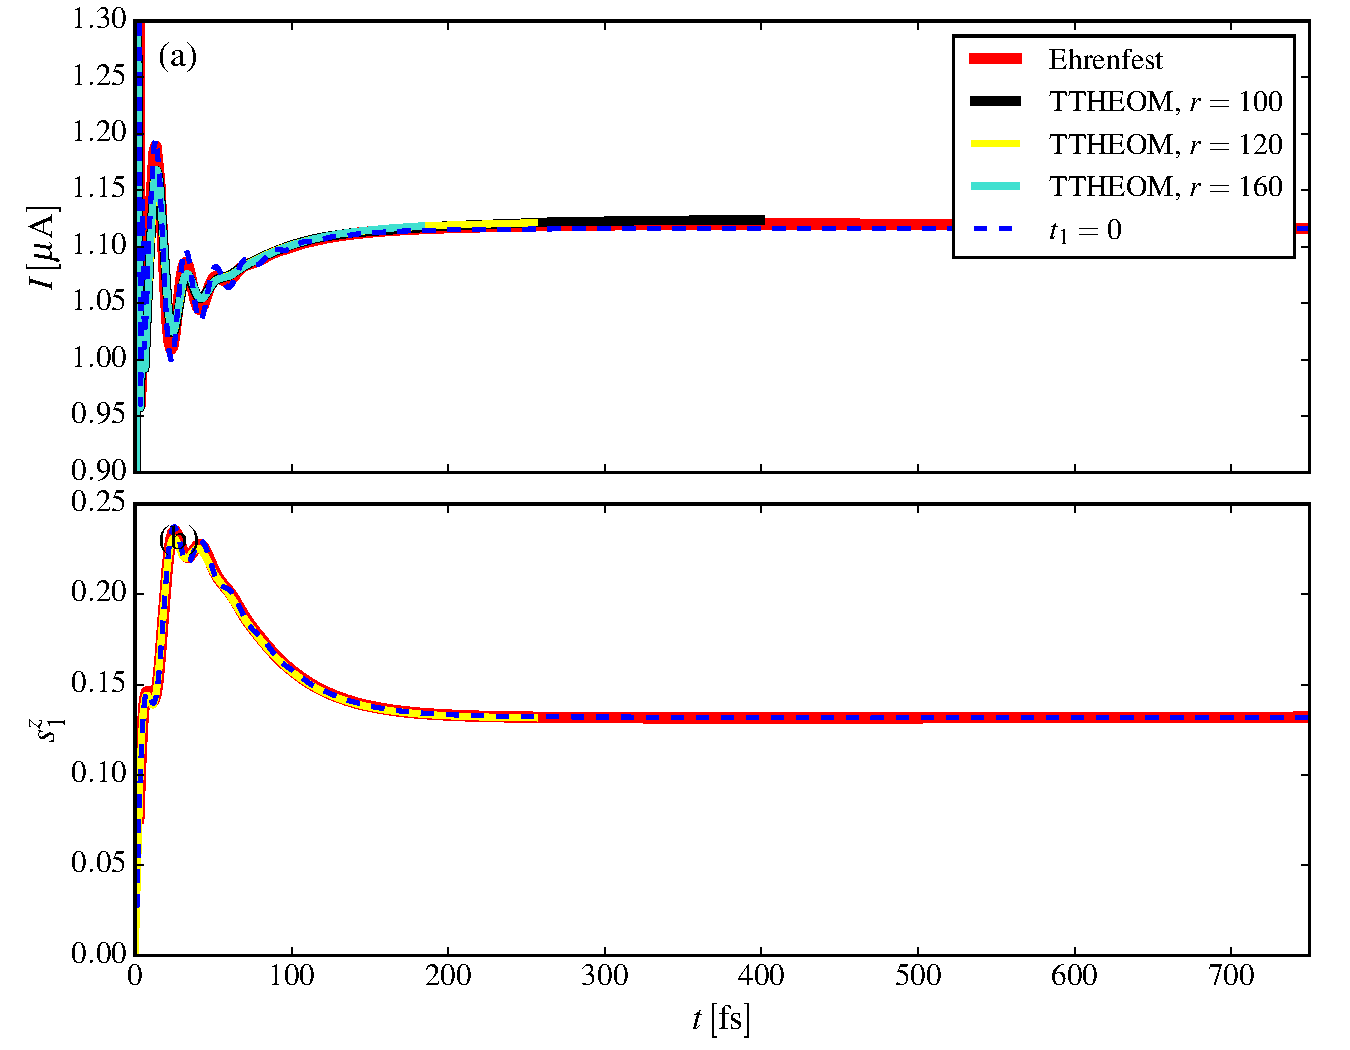
\includegraphics[width=0.9\textwidth]{figs/TTHEOM/L2_comparison_TTHEOM_MFHEOM_v3_PVar.pdf}
	\caption{Ehrenfest: $n=1500$. TTHEOM: $n_\mathrm{vib}=30$. Initial state in both approaches: Empty molecule and vibration in zero temperature ground state.} \label{fig:1}
\end{figure}
\subsubsection{$L=1\times 3$}
\Cref{fig:2} shows the current and the electronic spin polarization for the same parameters as in the previous section, with spin orbit coupling parameter $\lambda_0=\SI{1}{\milli\electronvolt}$ and $\lambda_1 = \SI{0.1}{\milli\electronvolt}$ and for a system size $L=1\times 3$. \Cref{fig:3} shows the dynamics of the magnetoresistance $M_R$. In the Ehrenfest approach, the magnetoresistance for this system size is numerically zero. 
\begin{figure}[!h]
	\centering
	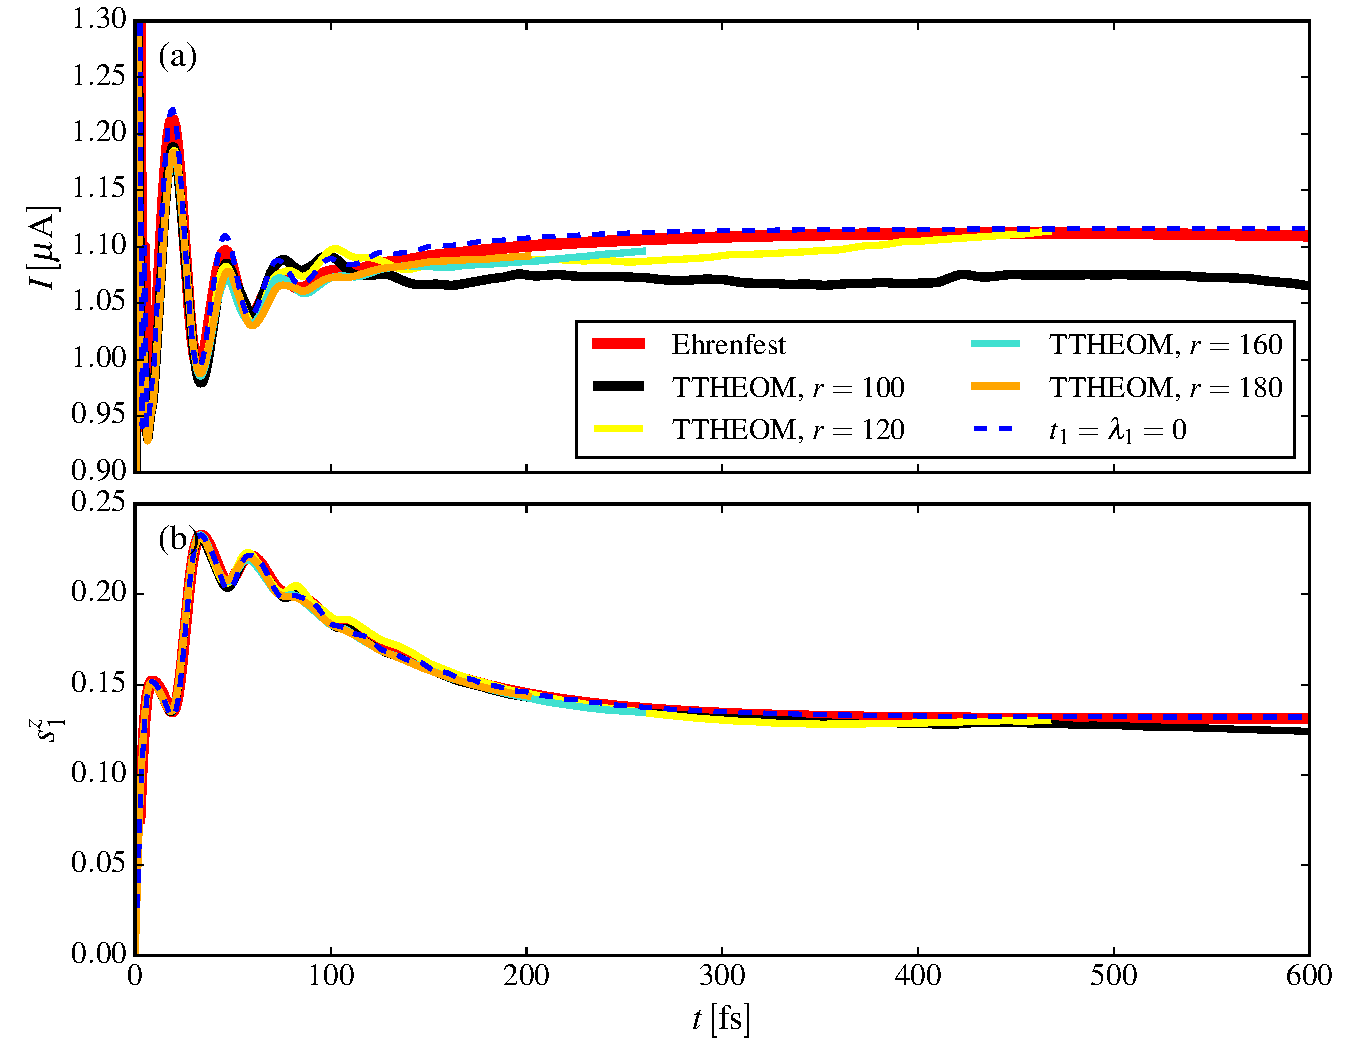
\includegraphics[width=0.9\textwidth]{figs/TTHEOM/L3_comparison_TTHEOM_MFHEOM_v3_PVar.pdf}
	\caption{Ehrenfest: $n=1275$. TTHEOM: $n_\mathrm{vib}=30$. } \label{fig:2}
\end{figure}
\begin{figure}[!h]
	\centering
	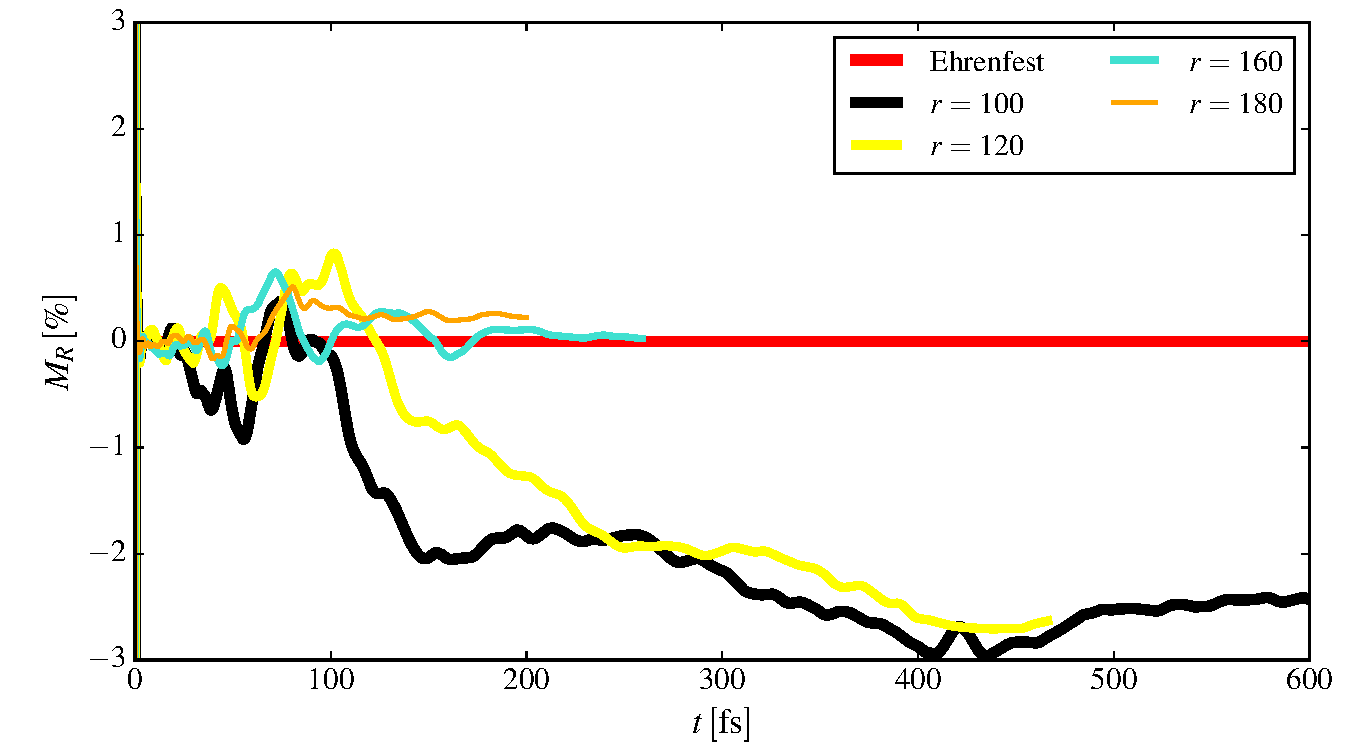
\includegraphics[width=0.9\textwidth]{figs/TTHEOM/L3_comparison_MR_TTHEOM_PVar.pdf}
	\caption{Magnetoresistance. Ehrenfest: $n=1275$. TTHEOM: $n_\mathrm{vib}=30$.} \label{fig:3}
\end{figure}
\subsubsection{Norm of state}
The norm of the state at each time step $\langle \!\langle \mathds{1}\vert \rho(t)\rangle\!\rangle$ is shown in \cref{fig:4}. Solid lines depict the norm for $L=1\times 2$ and dashed ones for $L=1\times 3$. 
\begin{figure}[!h]
	\centering
	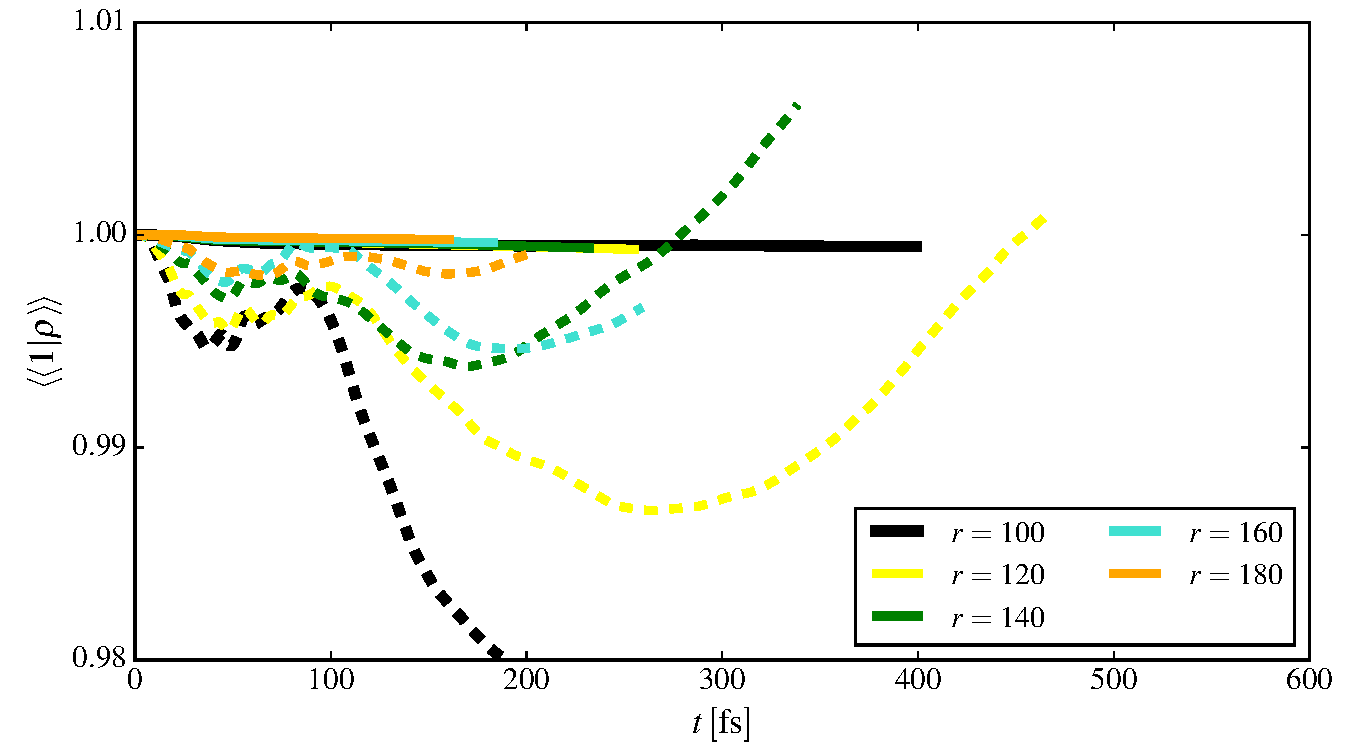
\includegraphics[width=0.9\textwidth]{figs/TTHEOM/Norm_TTHEOM_rankVar_LVar.pdf}
	\caption{Norm of state for varying rank. Solid lines show $L=1\times 2$ and dashed ones $L=1\times 3$.}\label{fig:4}
\end{figure}
\subsection{Spinless Peierls model $L=3$: Comparison to Ehrenfest-HEOM (August 8th report 16)}
\begin{figure}[!h]
	\centering
	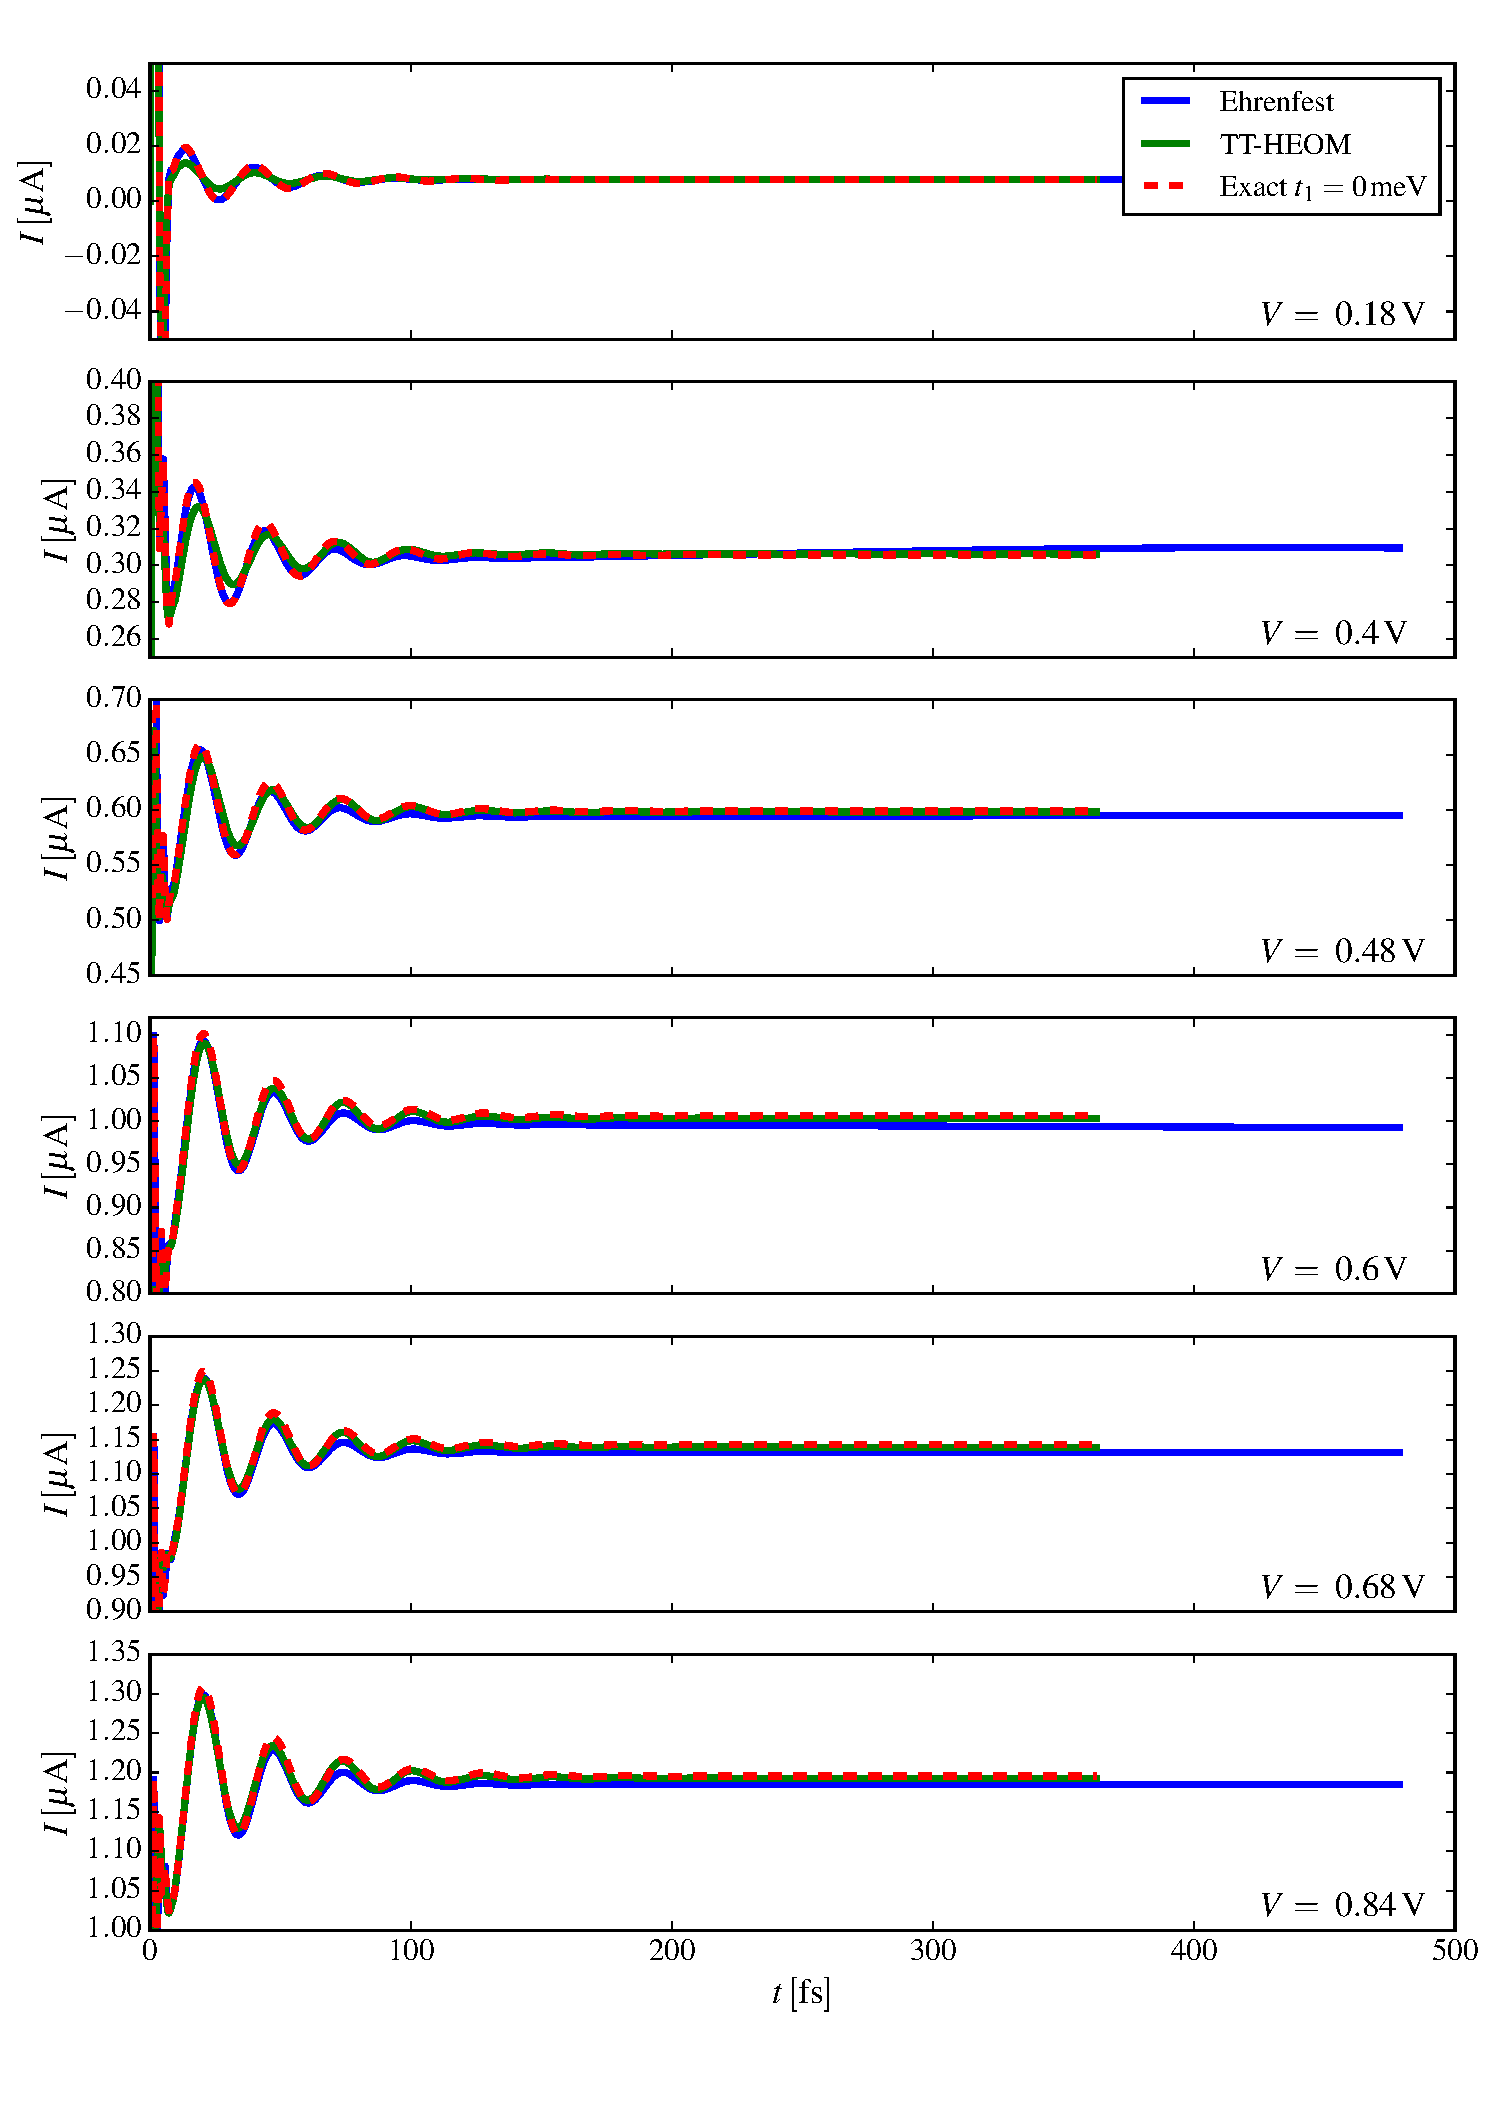
\includegraphics[width=0.9\textwidth]{figs/TTHEOM/Peierls_dyn_TTHEOM_Ehrenfest_noPh_VVar.pdf}
	\caption{Charge current dynamics in the three-site spinless Peierls model with $t_1=\SI{4}{\milli\electronvolt}$: Ehrenfest (blue), TT-HEOM (green) and the exact, noninteracting case (red dashed line). (Parameters are as in the original problem).}\label{fig:Comp_TTHEOM_Ehrenfest_t1_4meV}
\end{figure}
\clearpage
\section{Old Ehrenfest-HEOM results ($<$ August 20th)}
\subsection{System-size dependence of charge current}
This plot shows the system size dependence of the charge current in the Fransson model. The charge current has been obtained from ensemble-averaged currents, which have been time-averaged at the end of the simulation time. These results show that the electron-vibrational coupling leads to sub-diffusive electron dynamics, since the current has a power-law dependence on the system size with exponent $\gamma \approx \frac{1}{2}$. The voltage regime has been chosen in which the current depends almost linearly on voltage.
\begin{figure}[!h]
	\centering
	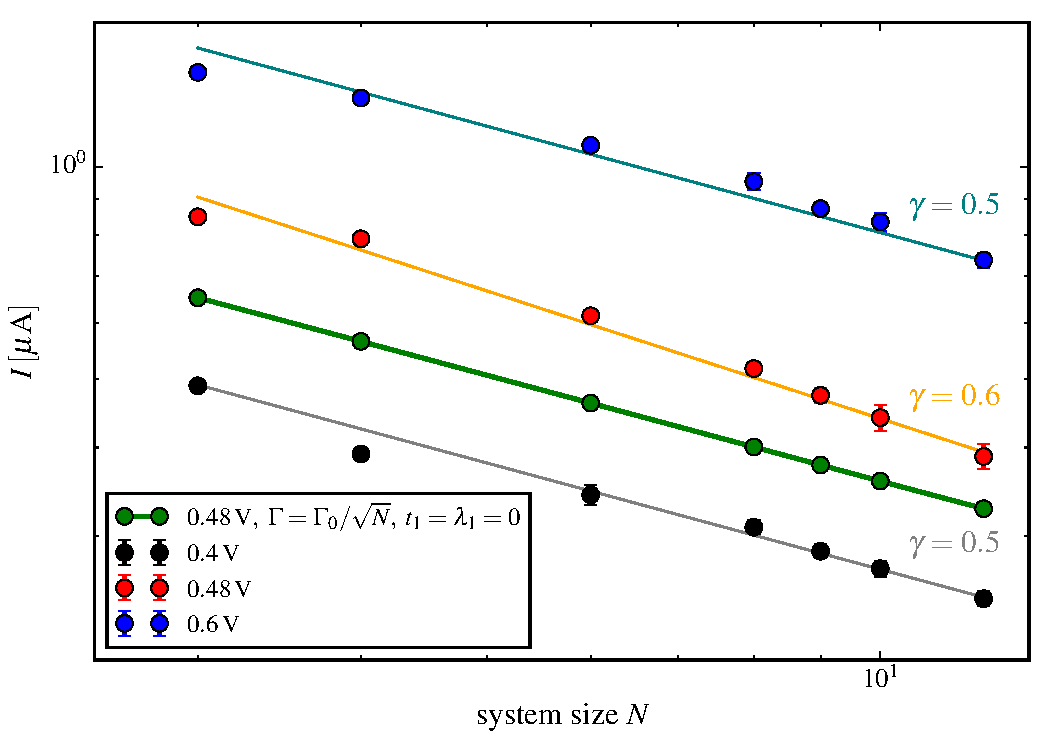
\includegraphics[width=0.65\textwidth]{figs/Old_MFHEOM/Currents_sizeVar_P0.5_VVar_log_slides.pdf}
	\caption{System-size dependence of charge currents for various charge currents obtained from steady state currents.}\label{fig:IV_Ndep}
\end{figure}
\subsection{System-size and voltage dependence of spin selectivity}
\begin{figure}[!h]
	\centering
	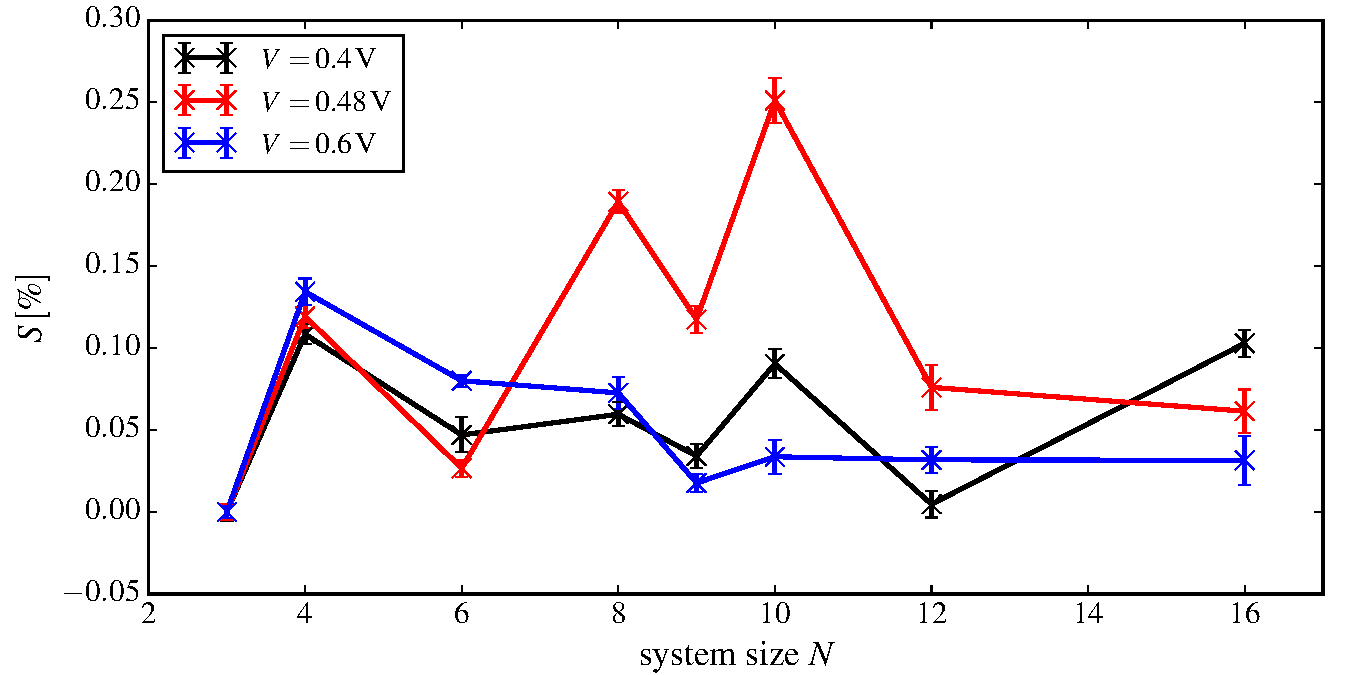
\includegraphics[width=0.8\textwidth]{figs/Old_MFHEOM/Spin_selectivity_sizeVar_VVar_stderr.pdf}
	\caption{Voltage dependence of spin selectivity for various system size. Magnetoresistance obtained from steady state currents.}\label{fig:MR_V}
\end{figure}

\clearpage
\section{Most recent Ehrenfest-HEOM results}
\subsection{$L=2\times 4$, $\lambda_0=\SI{1}{\milli\electronvolt}$, $\lambda_1=\SI{0.1}{\milli\electronvolt}$}
\subsubsection{Time-dependent electronic spectrum and voltage regimes}
\begin{figure}[!h]
	\centering
	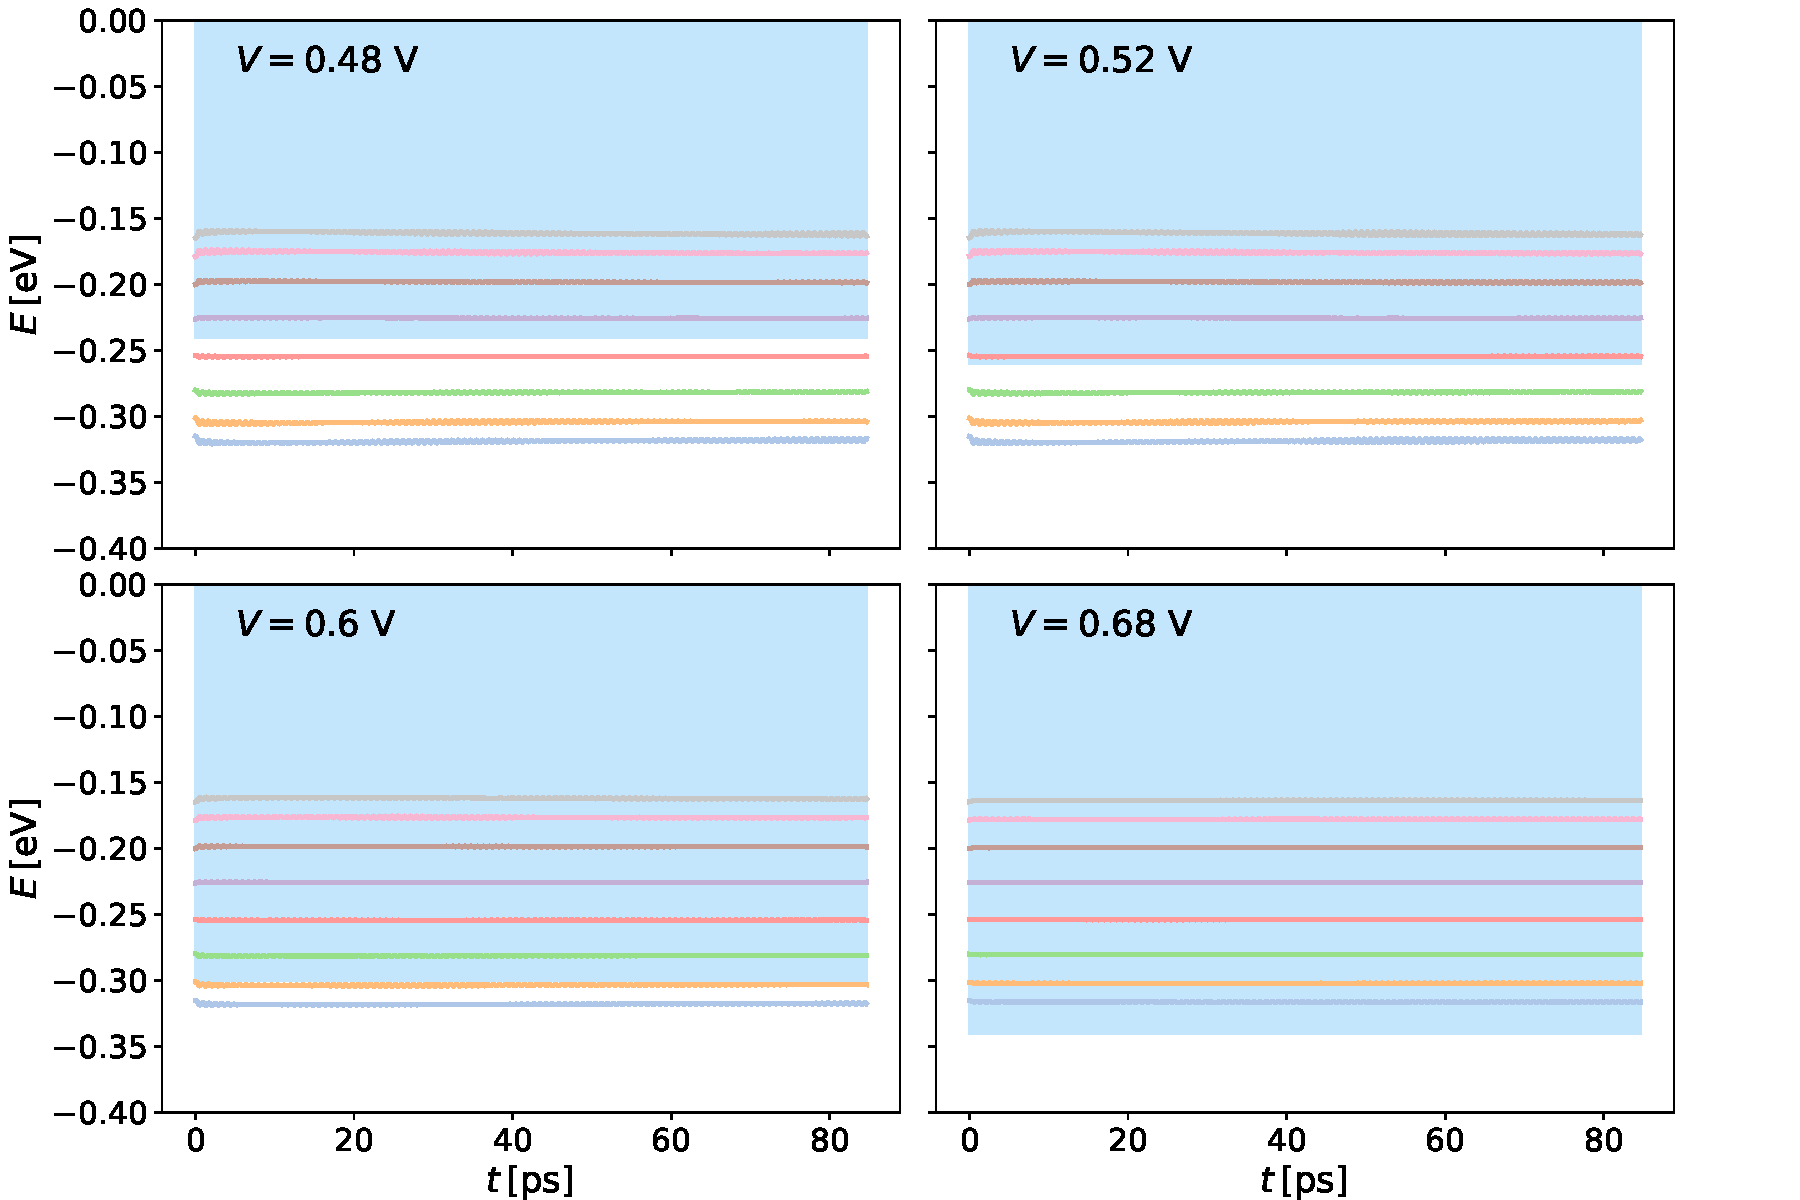
\includegraphics[width=0.9\textwidth]{figs/tsoPh0.1/L2x4_spectrumTD_PhAvg_tsoPh0.1.pdf}
	%~/PhD/projects/CISS_data/v2/I_V/w0_2_t1_4_tso_1_tsoPh_0.1/PVar/L2x4/v3/
	\caption{Time-dependent spectrum, obtained by diagonalizing the Hamiltonian for the vibrational time-evolution (ensemble-averaged) obtained within the Ehrenfest approach.}
\end{figure}
\clearpage
%\subsubsection{Time- and energy-dependent molecule-lead coupling}
%{\color{red} This is wrong. Update plots.}
%\begin{figure}[!h]
%	\centering
%	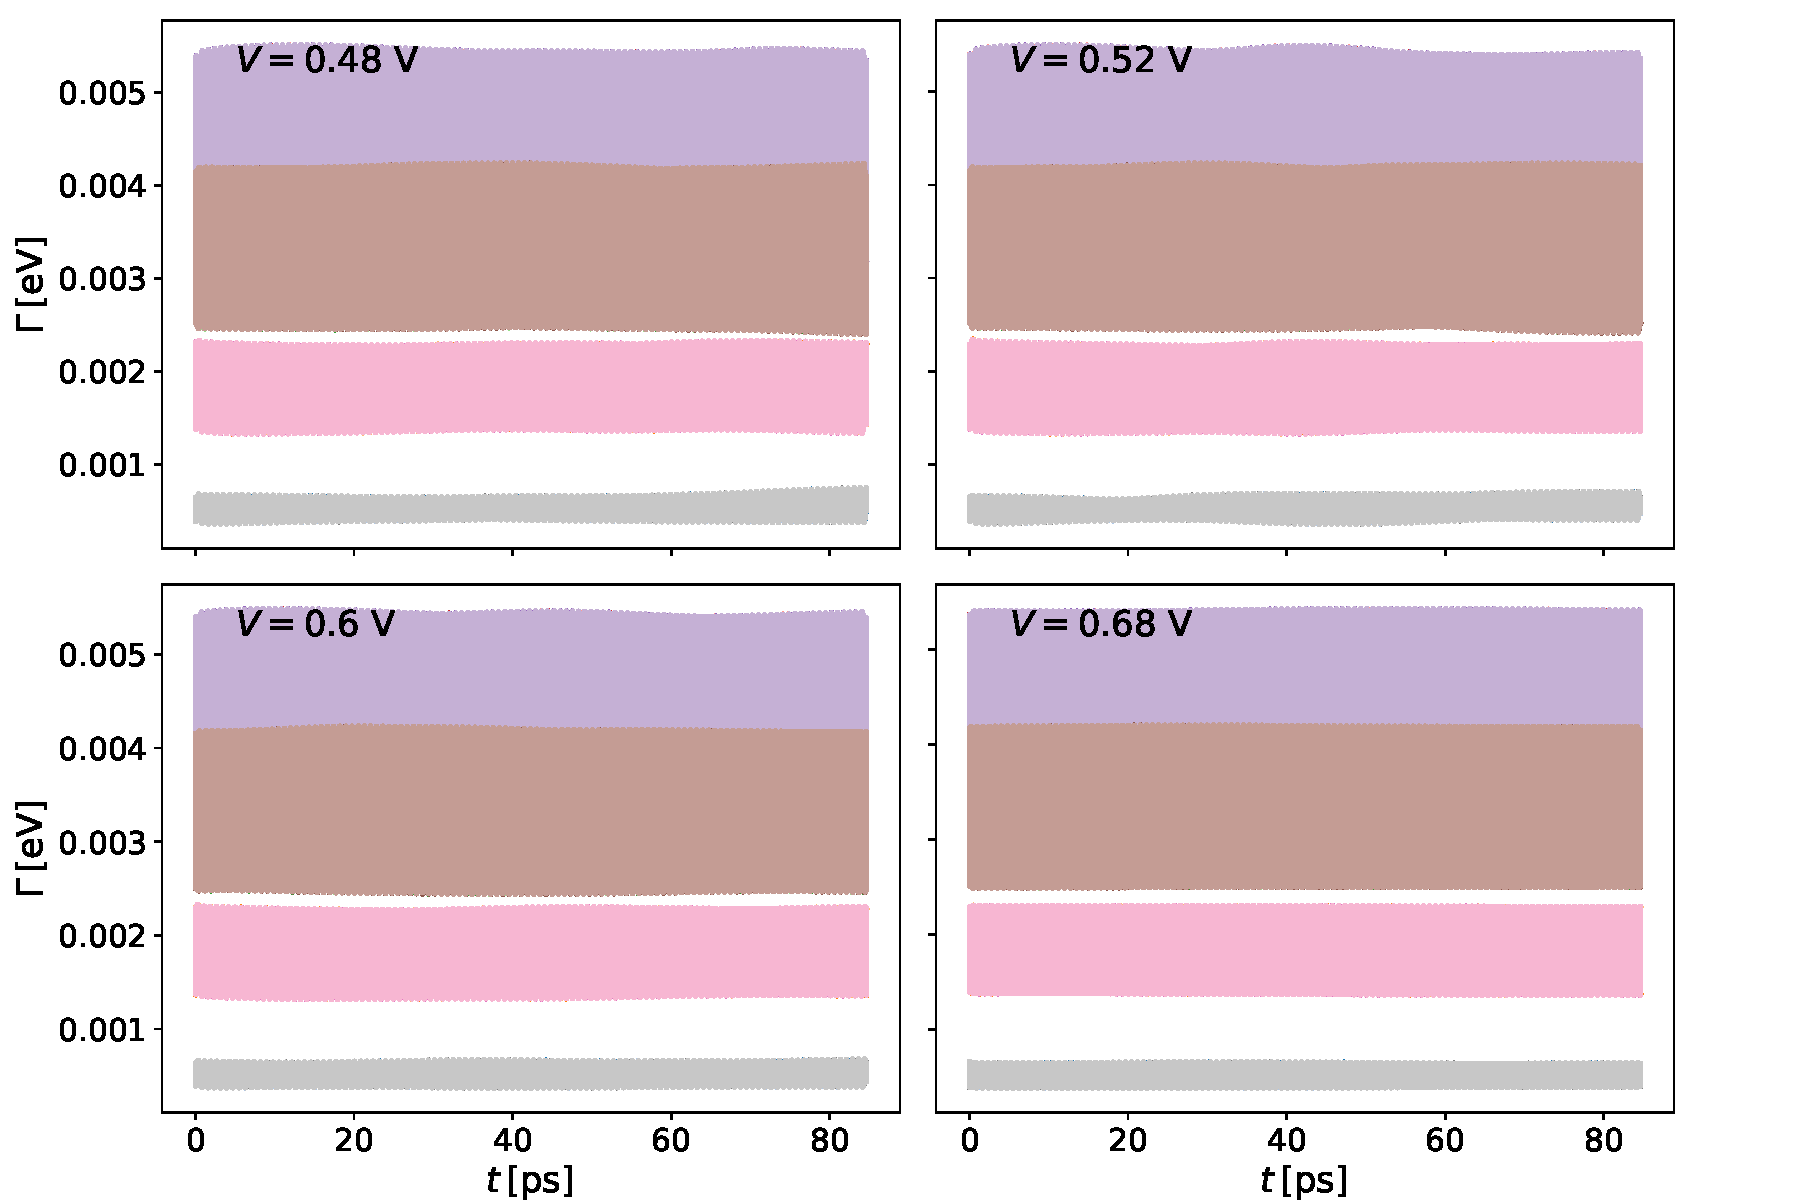
\includegraphics[width=0.9\textwidth]{figs/tsoPh0.1/L2x4_GammaTD_both_P_PhAvg_tsoPh0.1.pdf}
%	%~/PhD/projects/CISS_data/v2/I_V/w0_2_t1_4_tso_1_tsoPh_0.1/PVar/L2x4/v3/
%	\caption{Time-dependence of the energy-resolved molecule-lead coupling, also obtained by diagonalizing the time-dependent Hamiltonian for $P=0.5$.}
%\end{figure}
%\begin{figure}[!h]
%	\centering
%	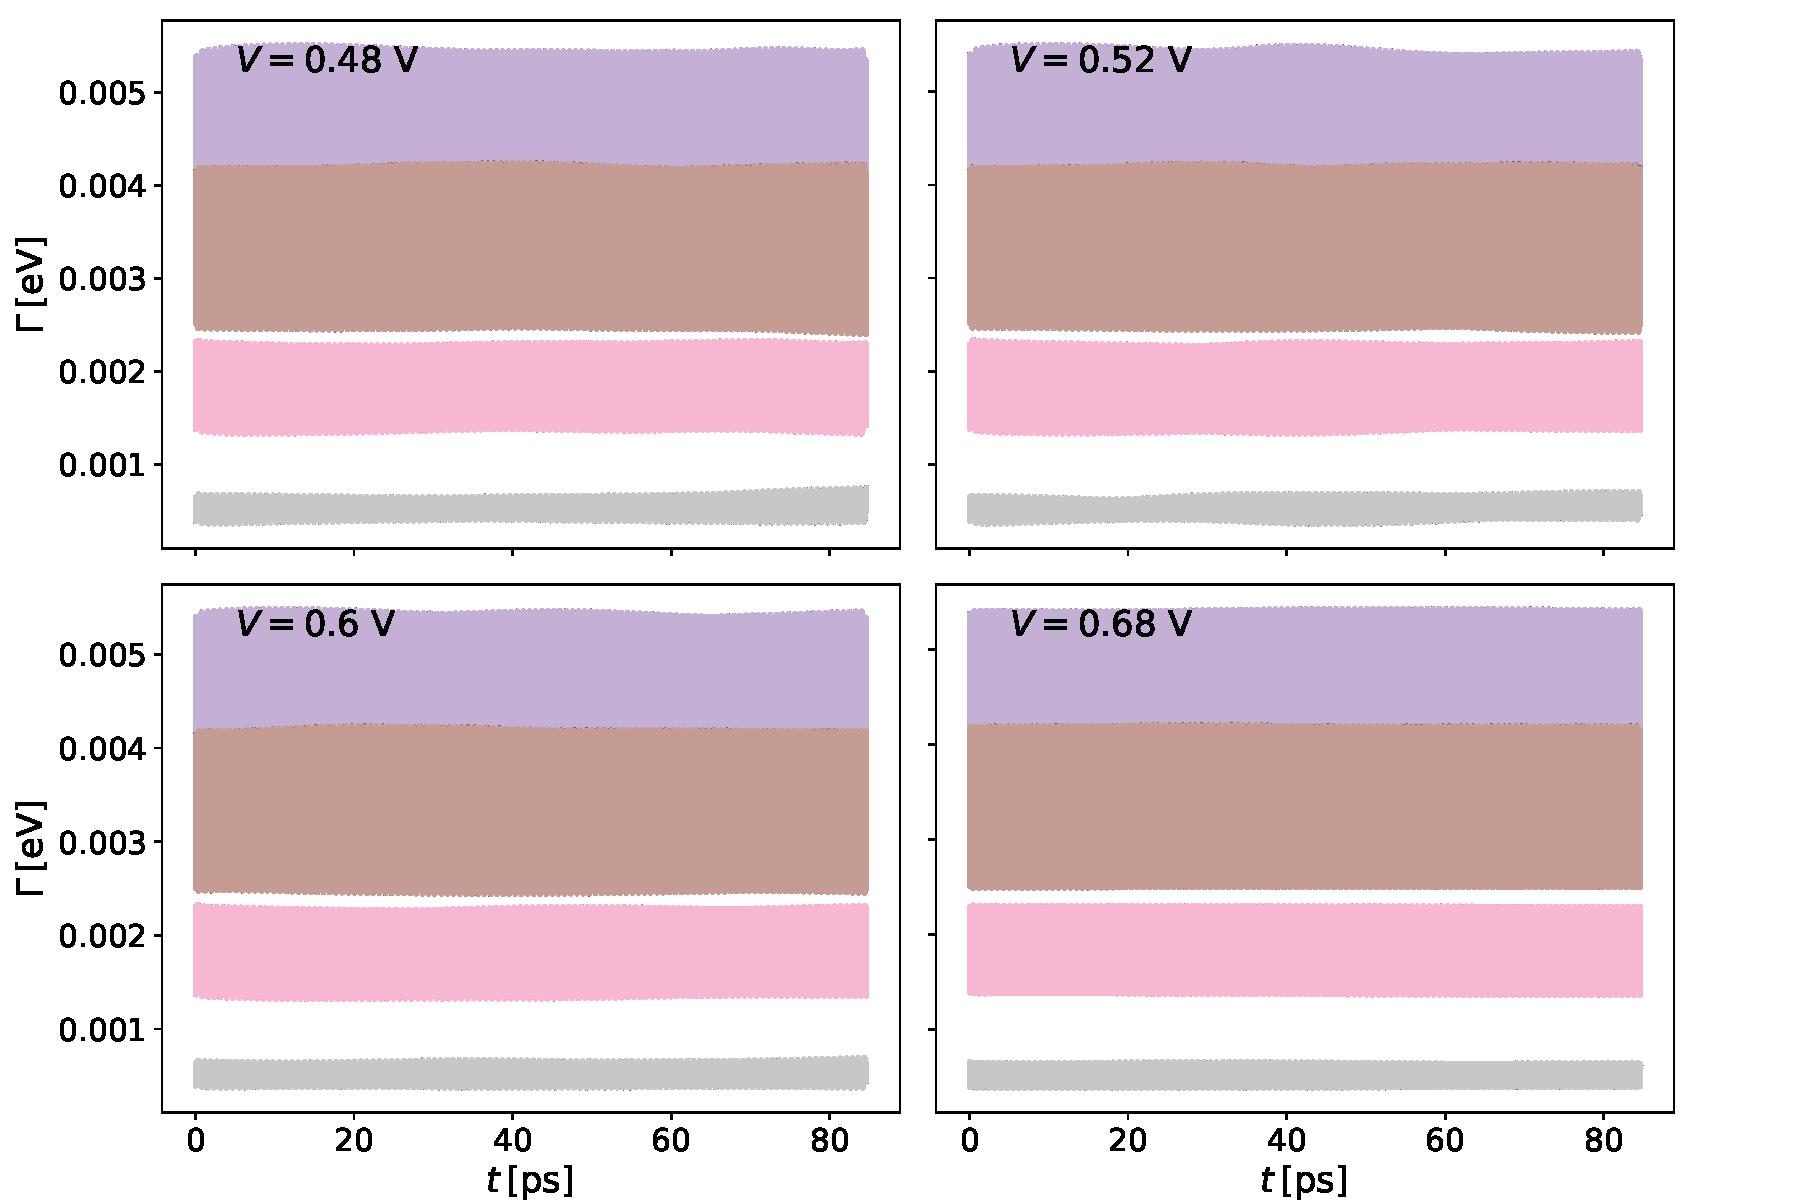
\includegraphics[width=0.9\textwidth]{figs/tsoPh0.1/L2x4_GammaTD_both_M_PhAvg_tsoPh0.1.pdf}
%	%~/PhD/projects/CISS_data/v2/I_V/w0_2_t1_4_tso_1_tsoPh_0.1/PVar/L2x4/v3/
%	\caption{Same as in the previous figure, but for $P=-0.5$.}
%\end{figure}
\subsubsection{Time-dependent charge currents and spin selectivity}
\begin{figure}[!h]
	\centering
	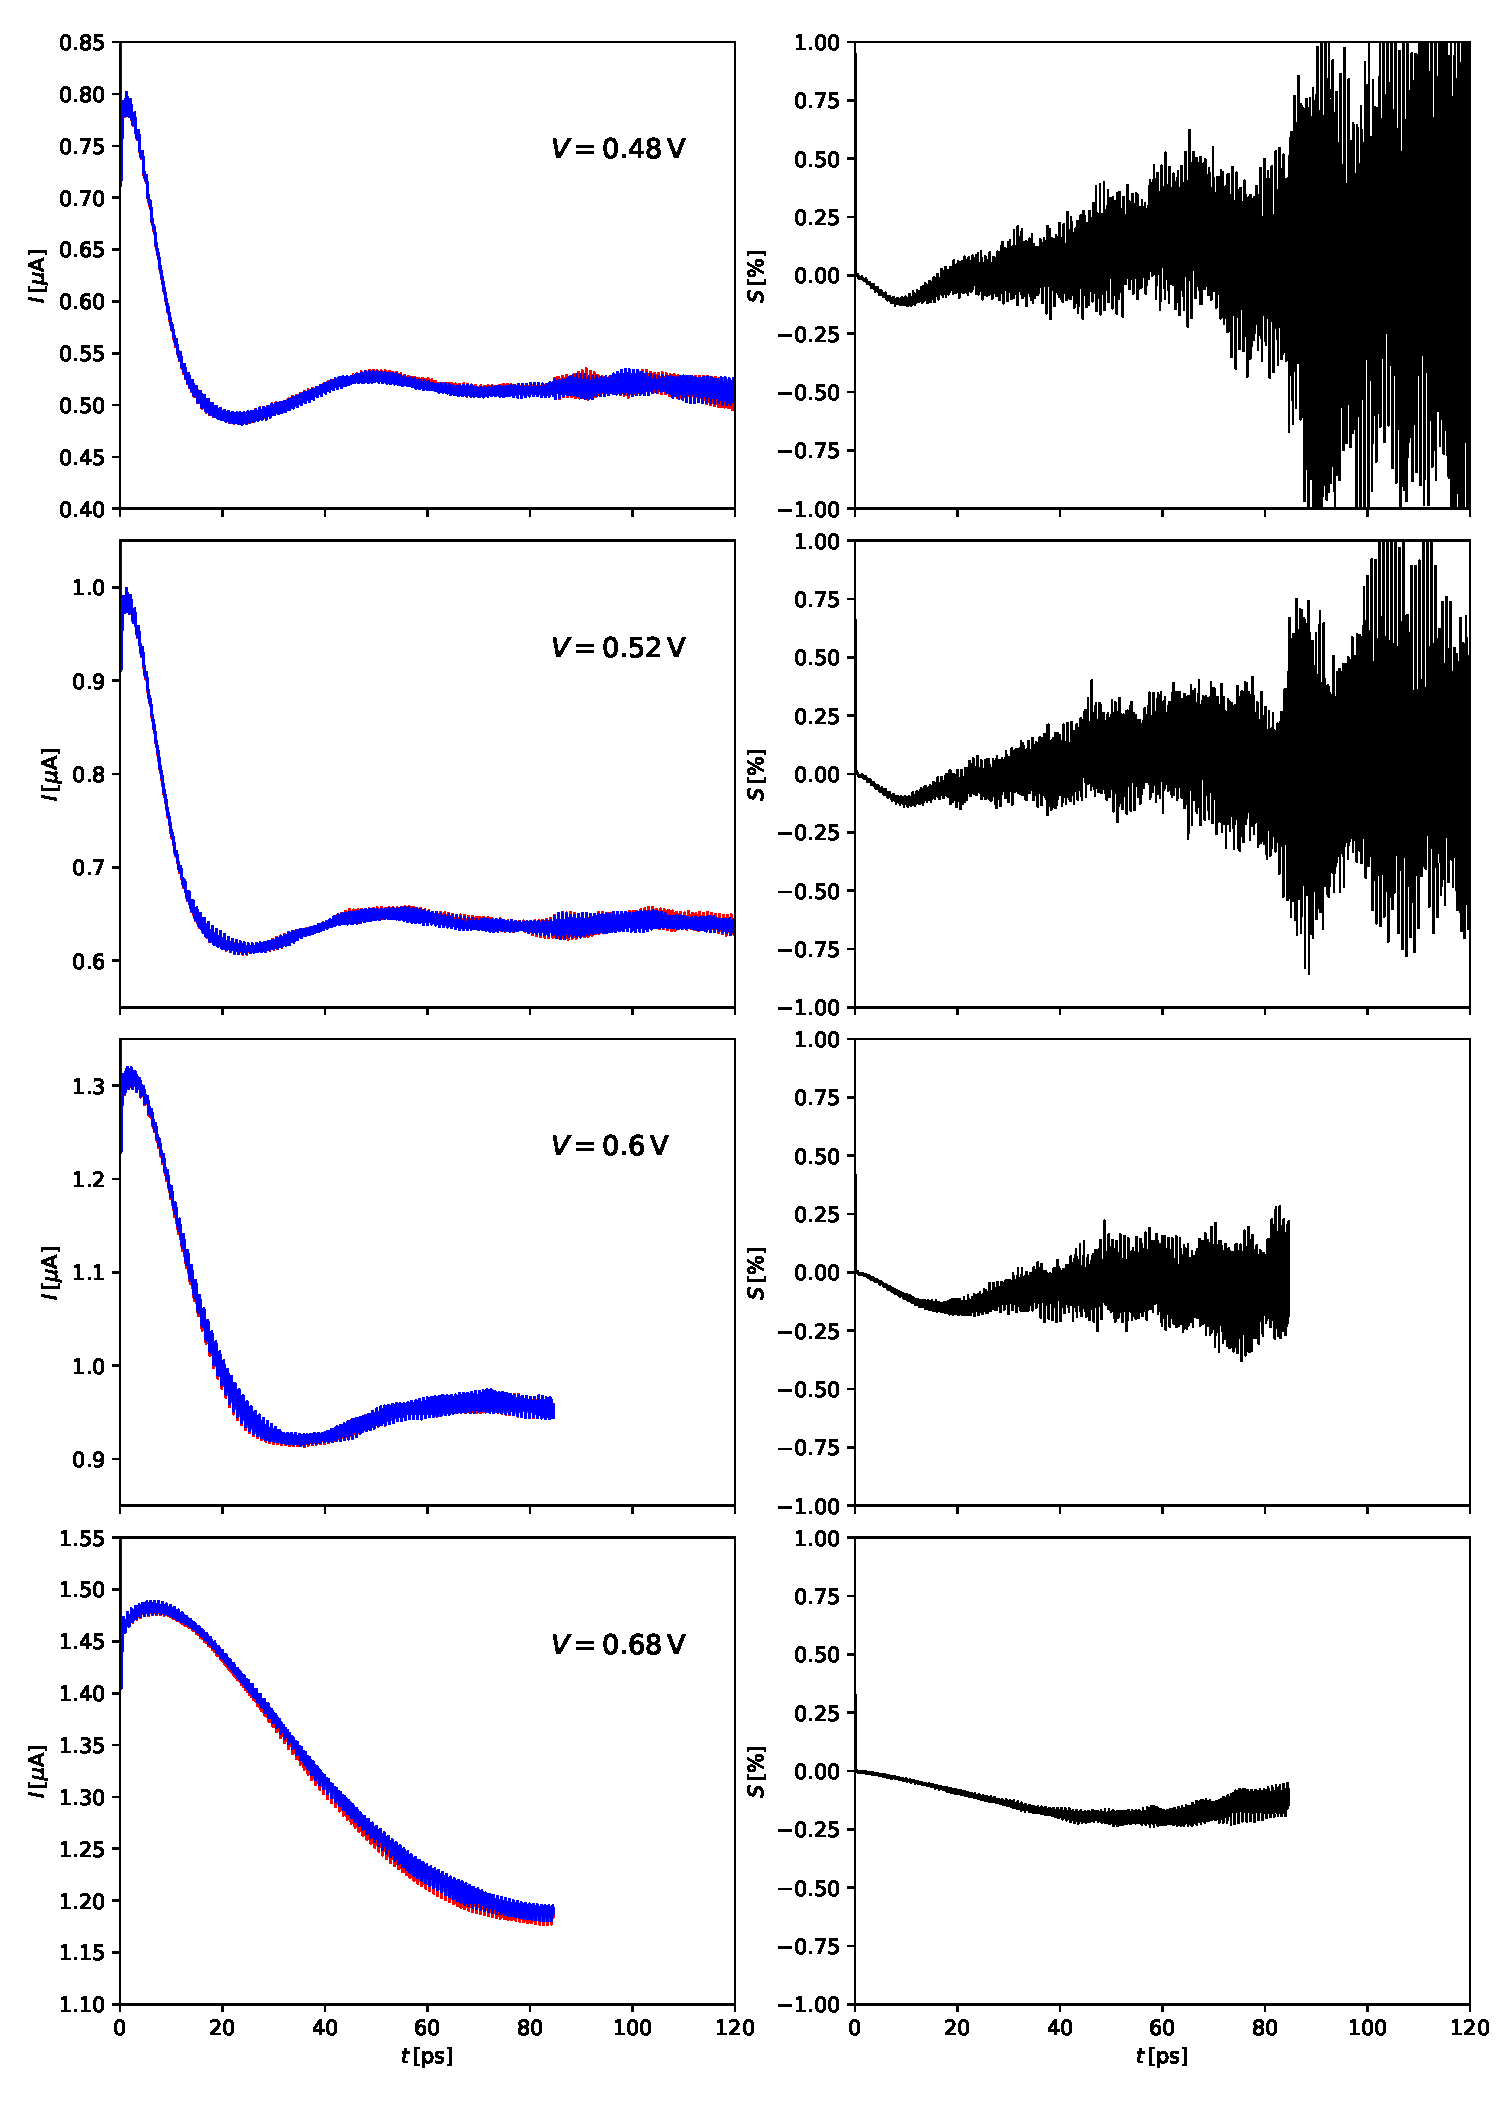
\includegraphics[width=0.9\textwidth]{figs/tsoPh0.1/L2x4_currents_MR_allV_tsoPh0.1.pdf}
	%~/PhD/projects/CISS_data/v2/I_V/w0_2_t1_4_tso_1_tsoPh_0.1/PVar/L2x4/v3/
	\caption{Ensemble-averaged current dynamics for $P=0.5$ (red curve) and $P=-0.5$ (blue curve) [left column] and spin selectivity $S$ [right column].}
\end{figure}
\subsubsection{Dynamics of total charge and total spin}
\begin{figure}[!h]
	\centering
	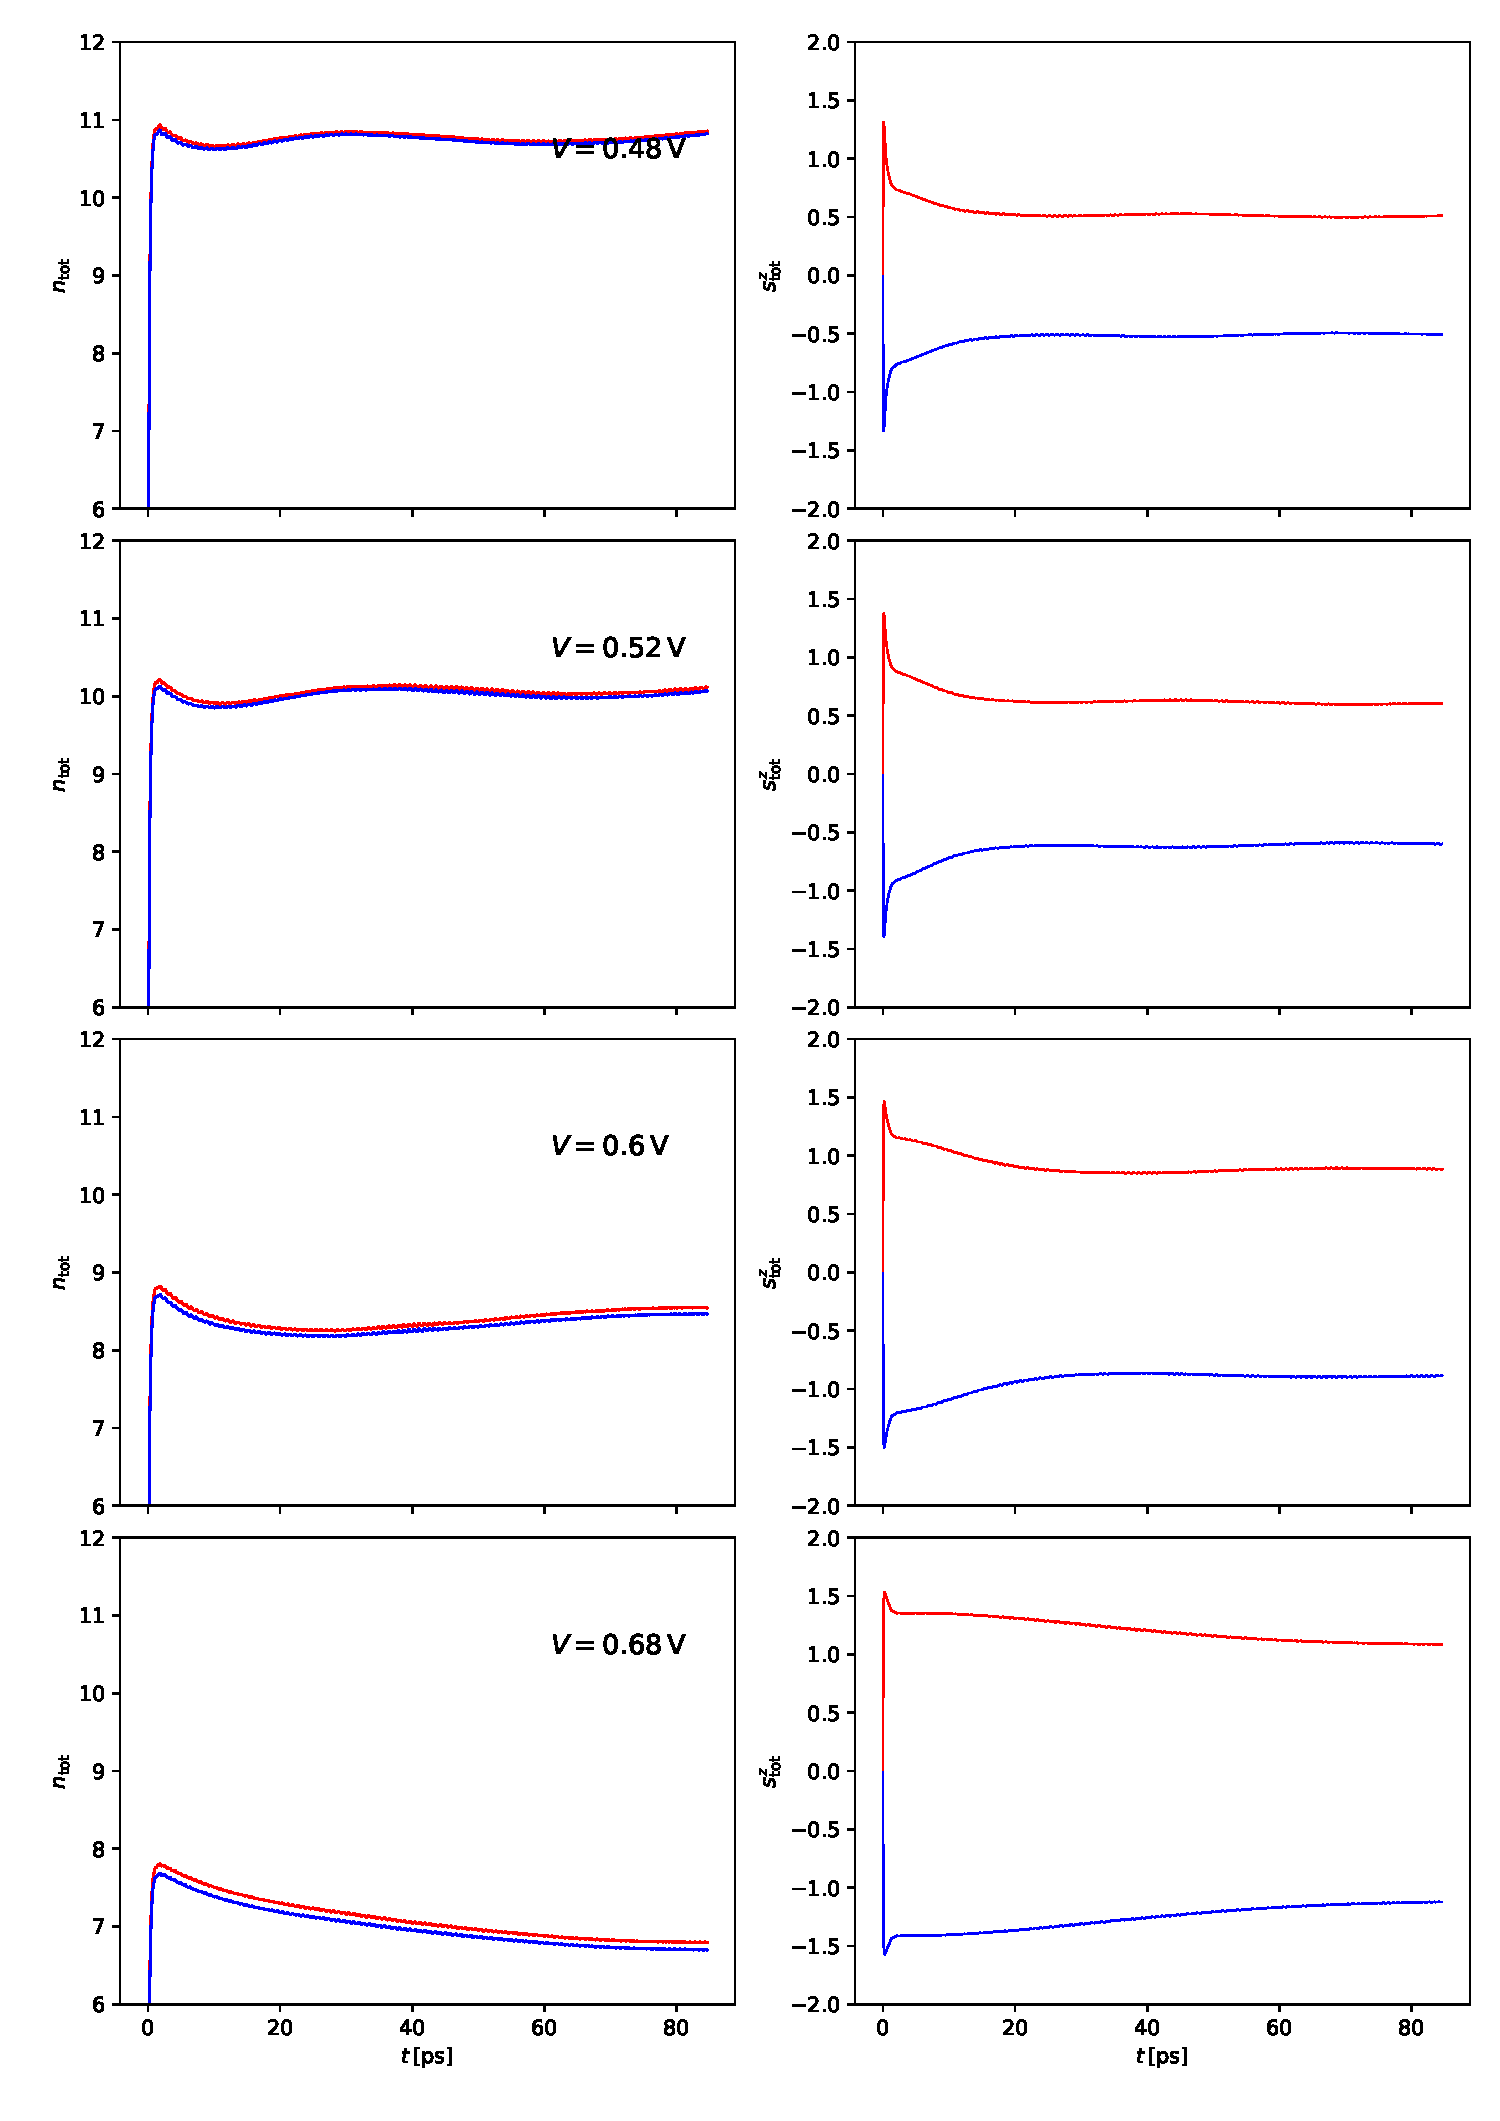
\includegraphics[width=0.9\textwidth]{figs/tsoPh0.1/L2x4_charge_sz_tot_allV_tsoPh0.1.pdf}
	%~/PhD/projects/CISS_data/v2/I_V/w0_2_t1_4_tso_1_tsoPh_0.1/PVar/L2x4/v3/
	\caption{Ensemble-averaged total charge [left column] and electron spin polarization dynamics [right column] for $P=0.5$ (red curve) and $P=-0.5$ (blue curve).}
\end{figure}
\subsubsection{Vibrational dynamics}
\begin{figure}[!h]
	\centering
	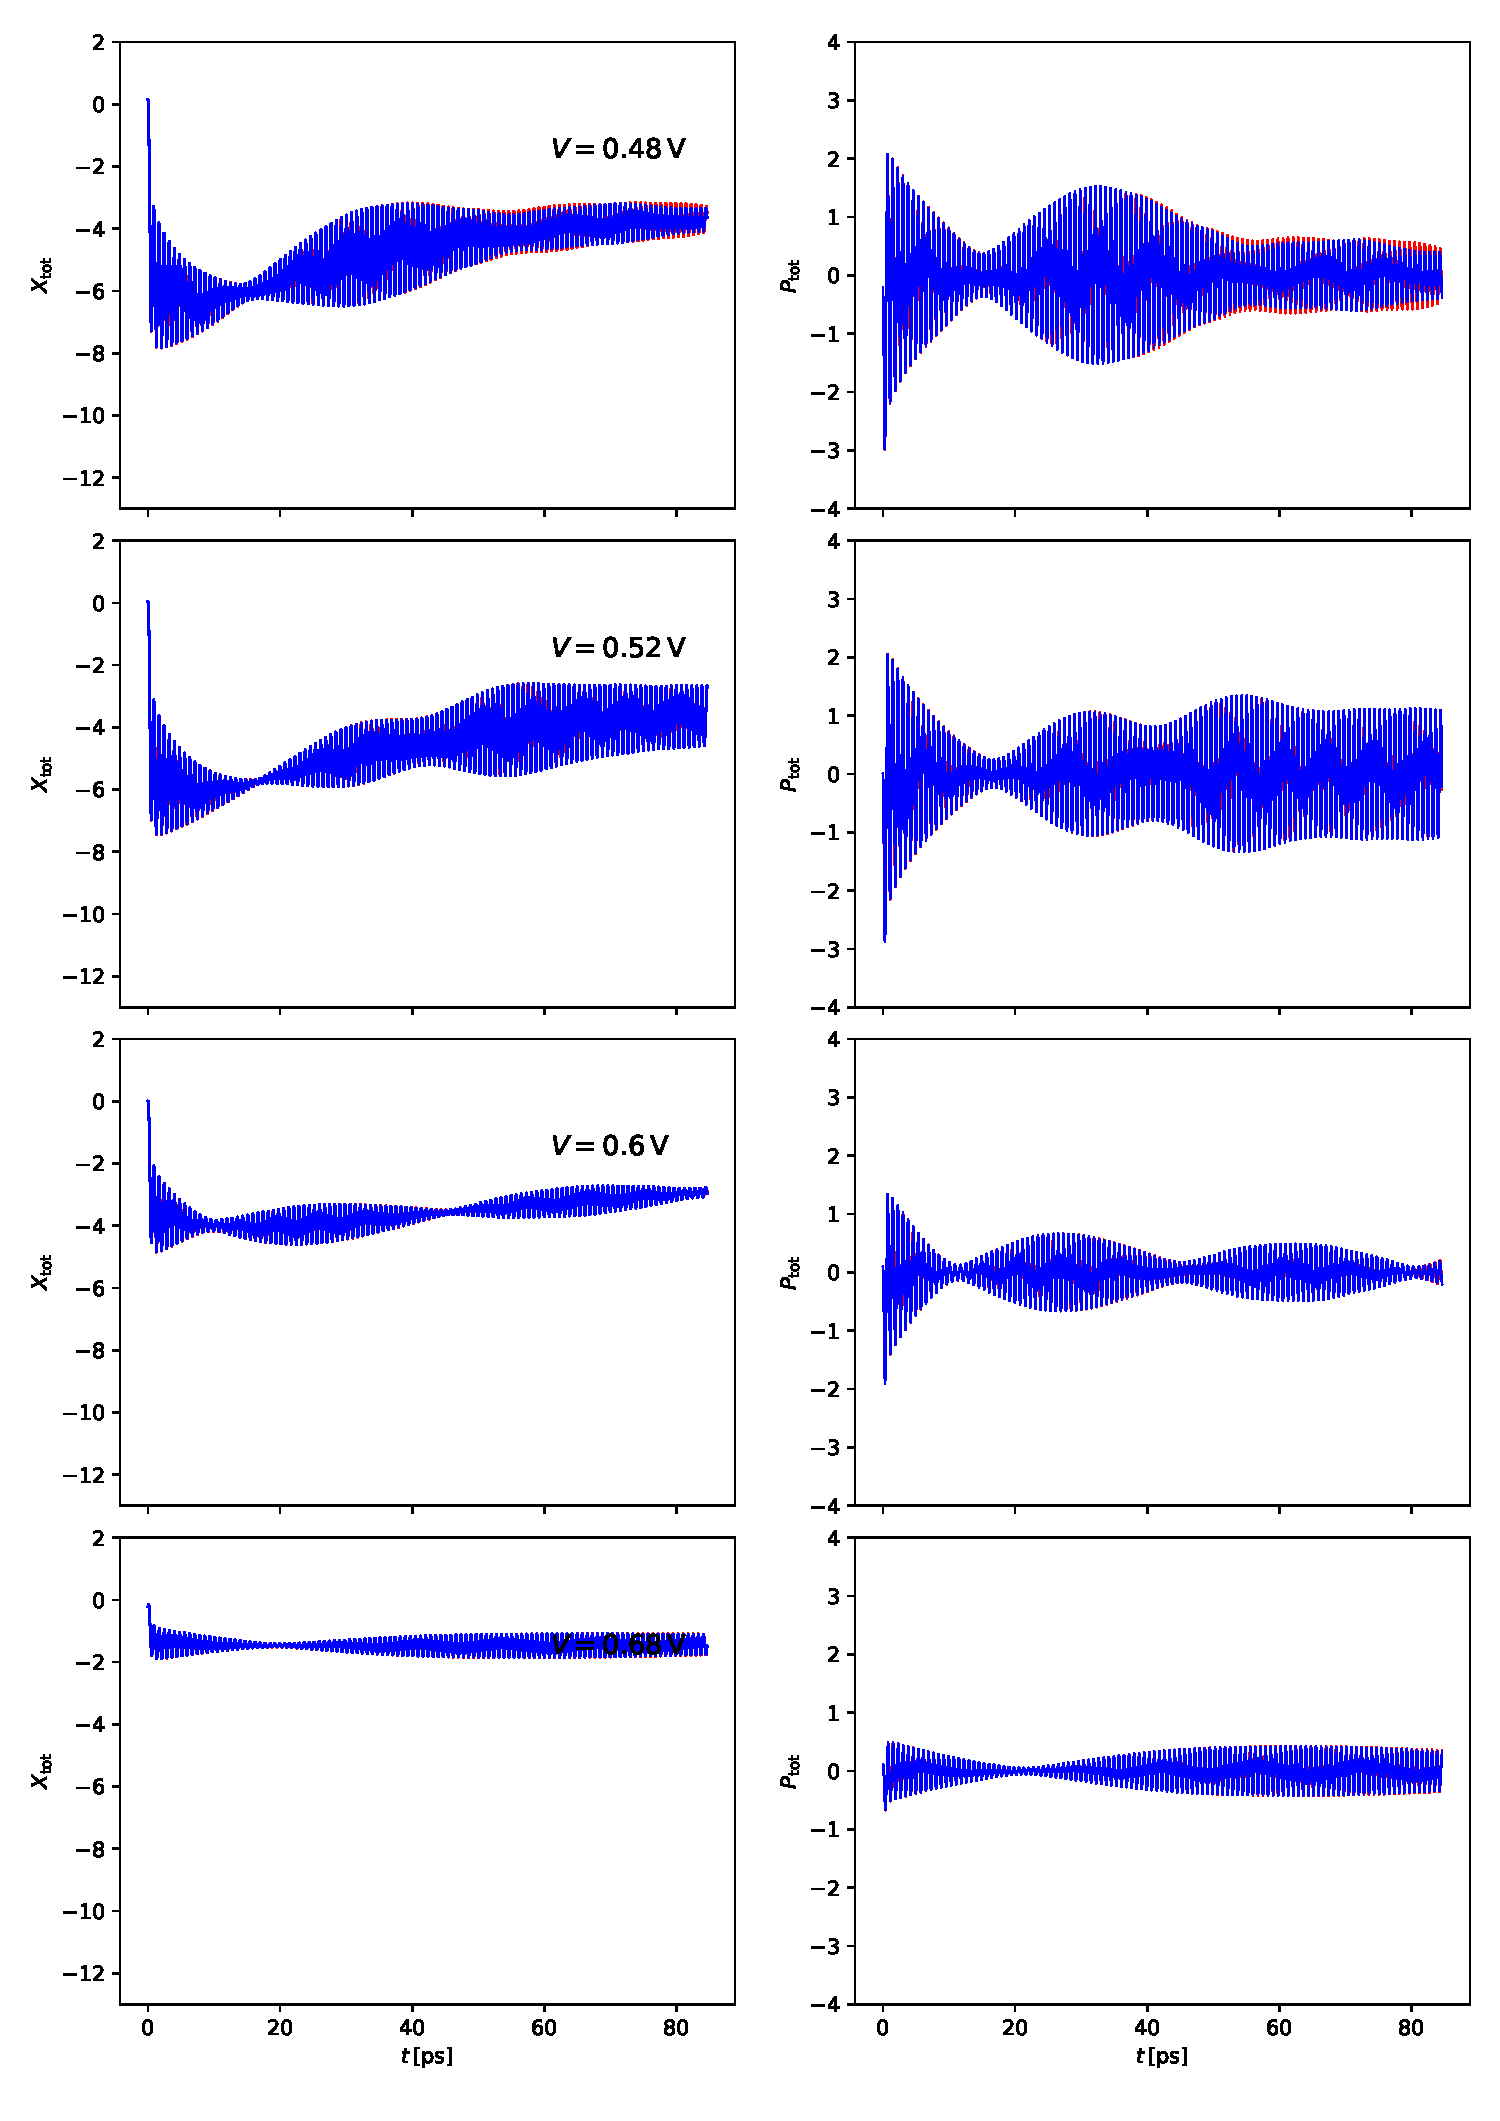
\includegraphics[width=0.9\textwidth]{figs/tsoPh0.1/L2x4_phonons_comb_allV_tsoPh0.1.pdf}
	%~/PhD/projects/CISS_data/v2/I_V/w0_2_t1_4_tso_1_tsoPh_0.1/PVar/L2x4/v3/
	\caption{Ensemble-averaged total phonon position [left column] and momentum dynamics [right column] for $P=0.5$ (red curve) and $P=-0.5$ (blue curve).}
\end{figure}
\subsubsection{Combined picture: Current, population and vibrational dynamics}
\begin{figure}[!h]
	\centering
	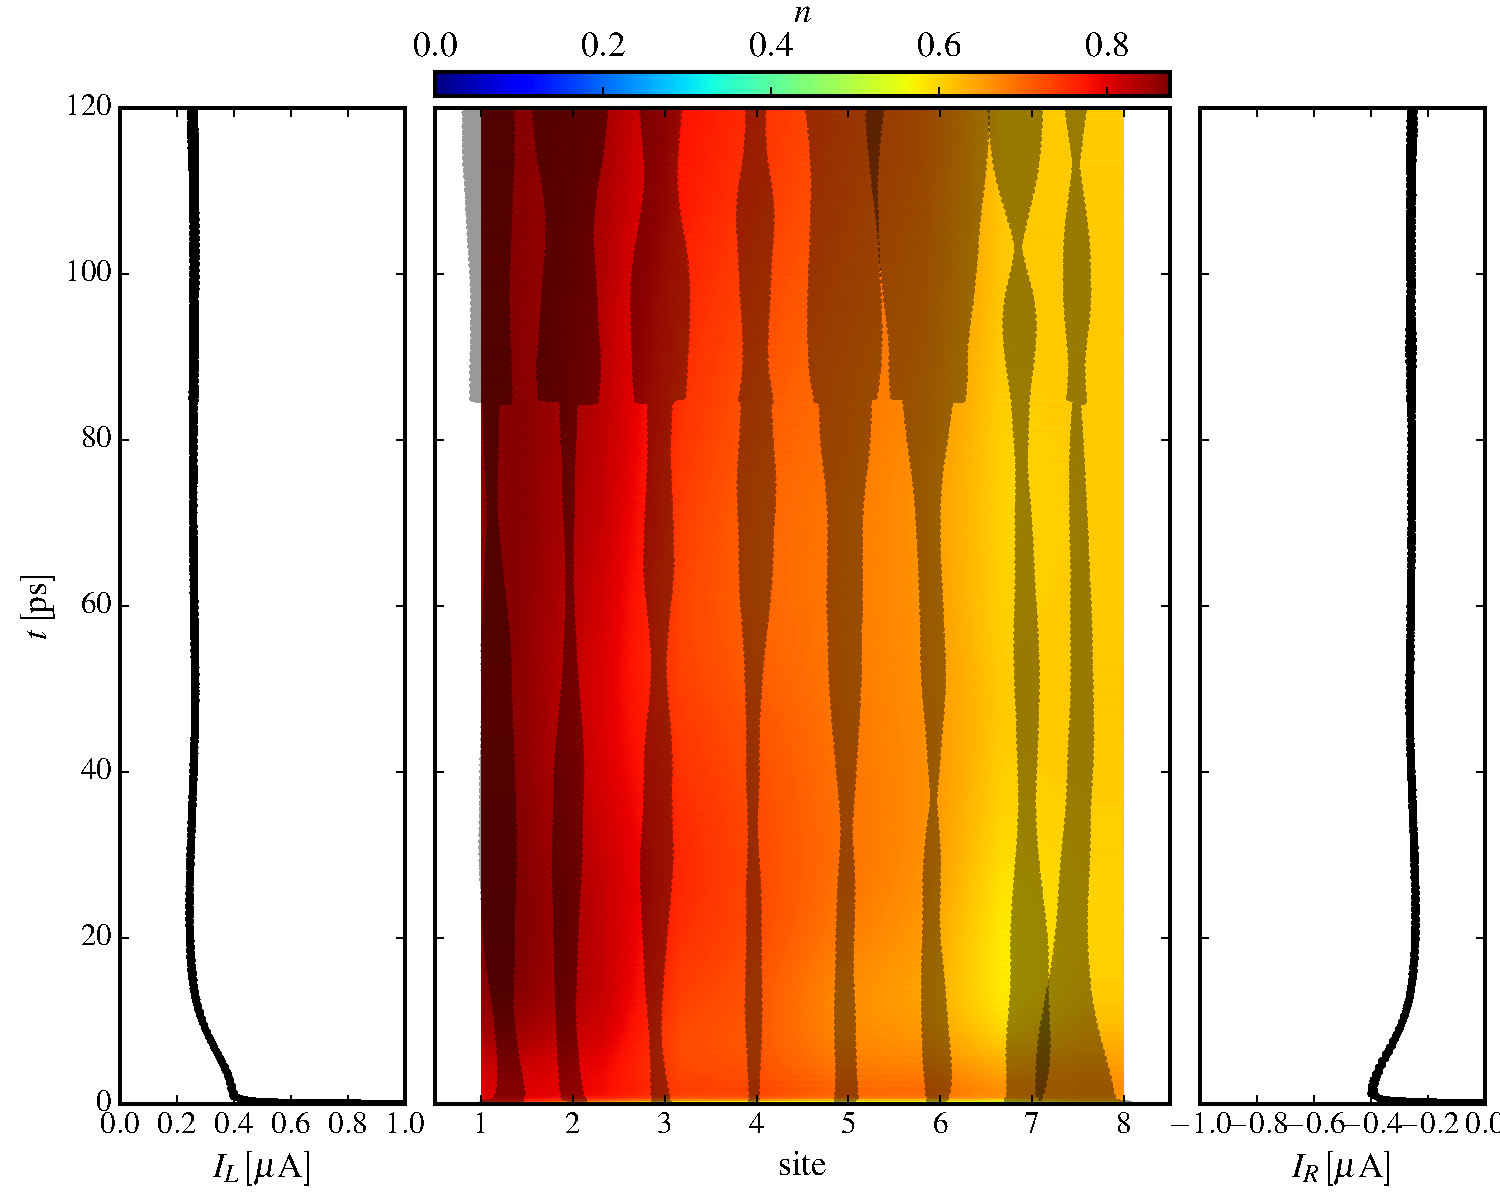
\includegraphics[width=0.8\textwidth]{figs/tsoPh0.1/L8_V60_tPh0.004_tso0.001_tsoPh0.0001_P_electrons_tend120_currents_phonons.pdf}
	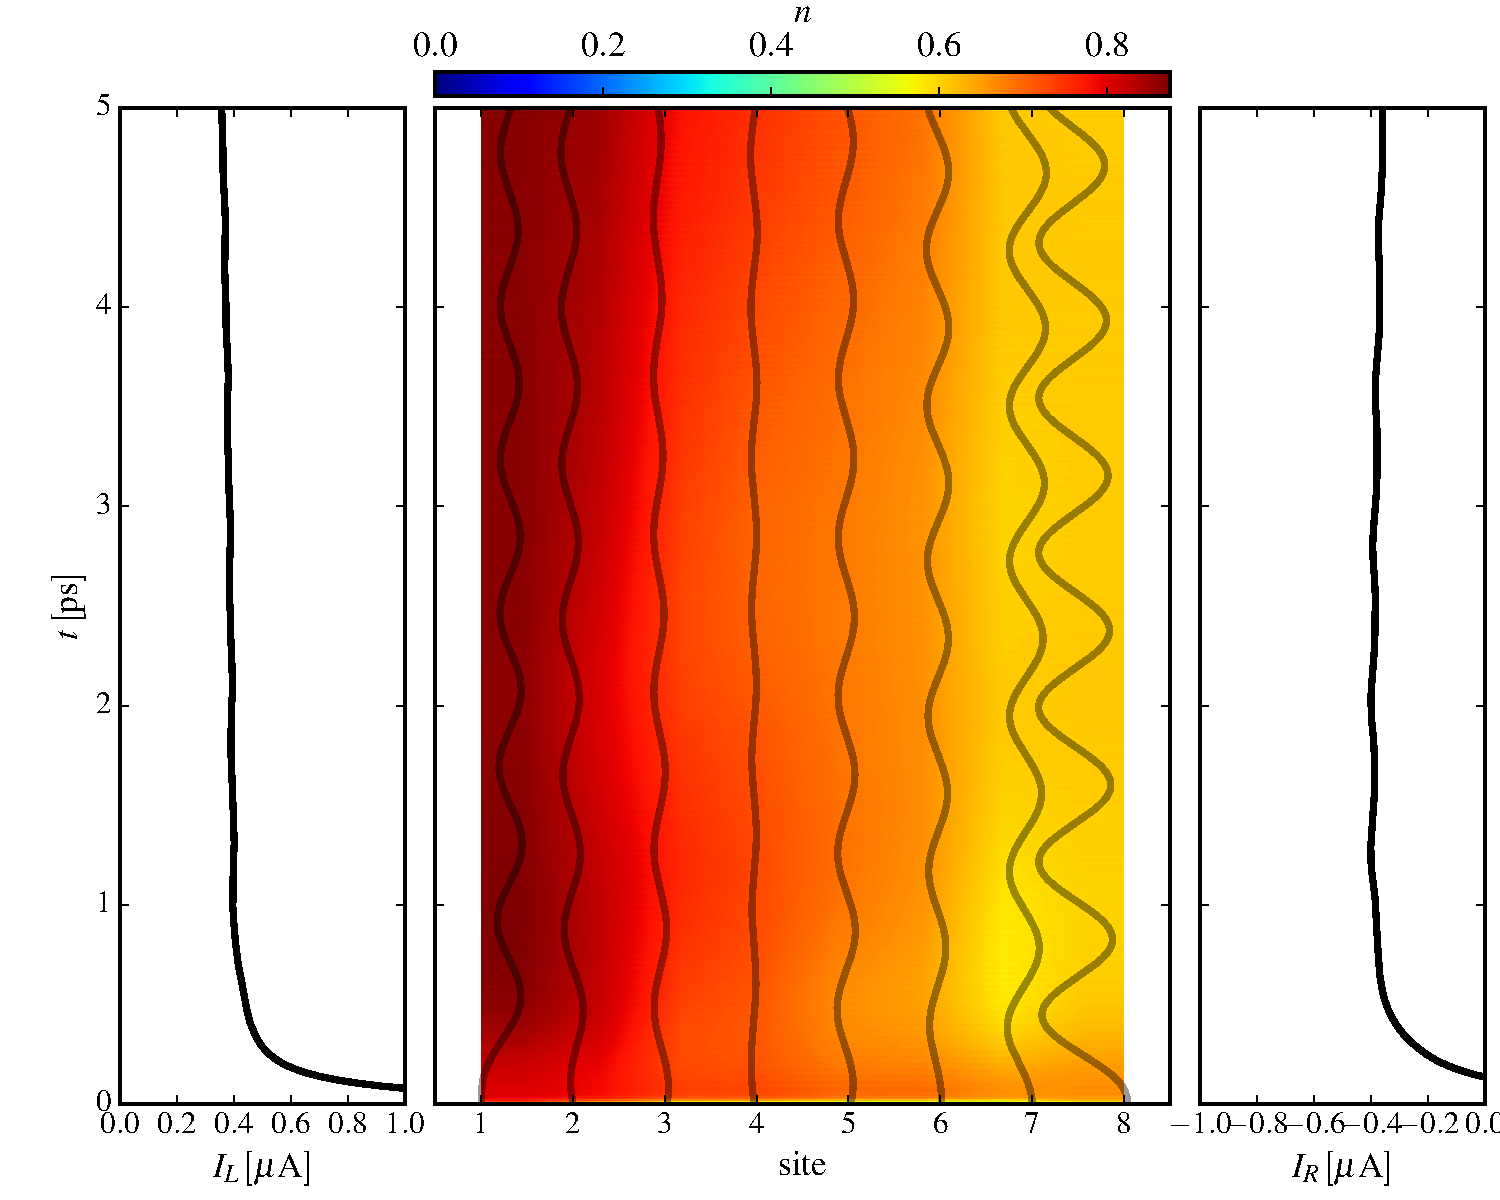
\includegraphics[width=0.8\textwidth]{figs/tsoPh0.1/L8_V60_tPh0.004_tso0.001_tsoPh0.0001_P_electrons_tend5_currents_phonons.pdf}
	%~/PhD/projects/CISS_data/v2/I_V/w0_2_t1_4_tso_1_tsoPh_0.1/PVar/L2x4/v3/
	\caption{For $V=\SI{0.48}{\volt}$, $P=0.5$.}
\end{figure}
\begin{figure}[!h]
	\centering
	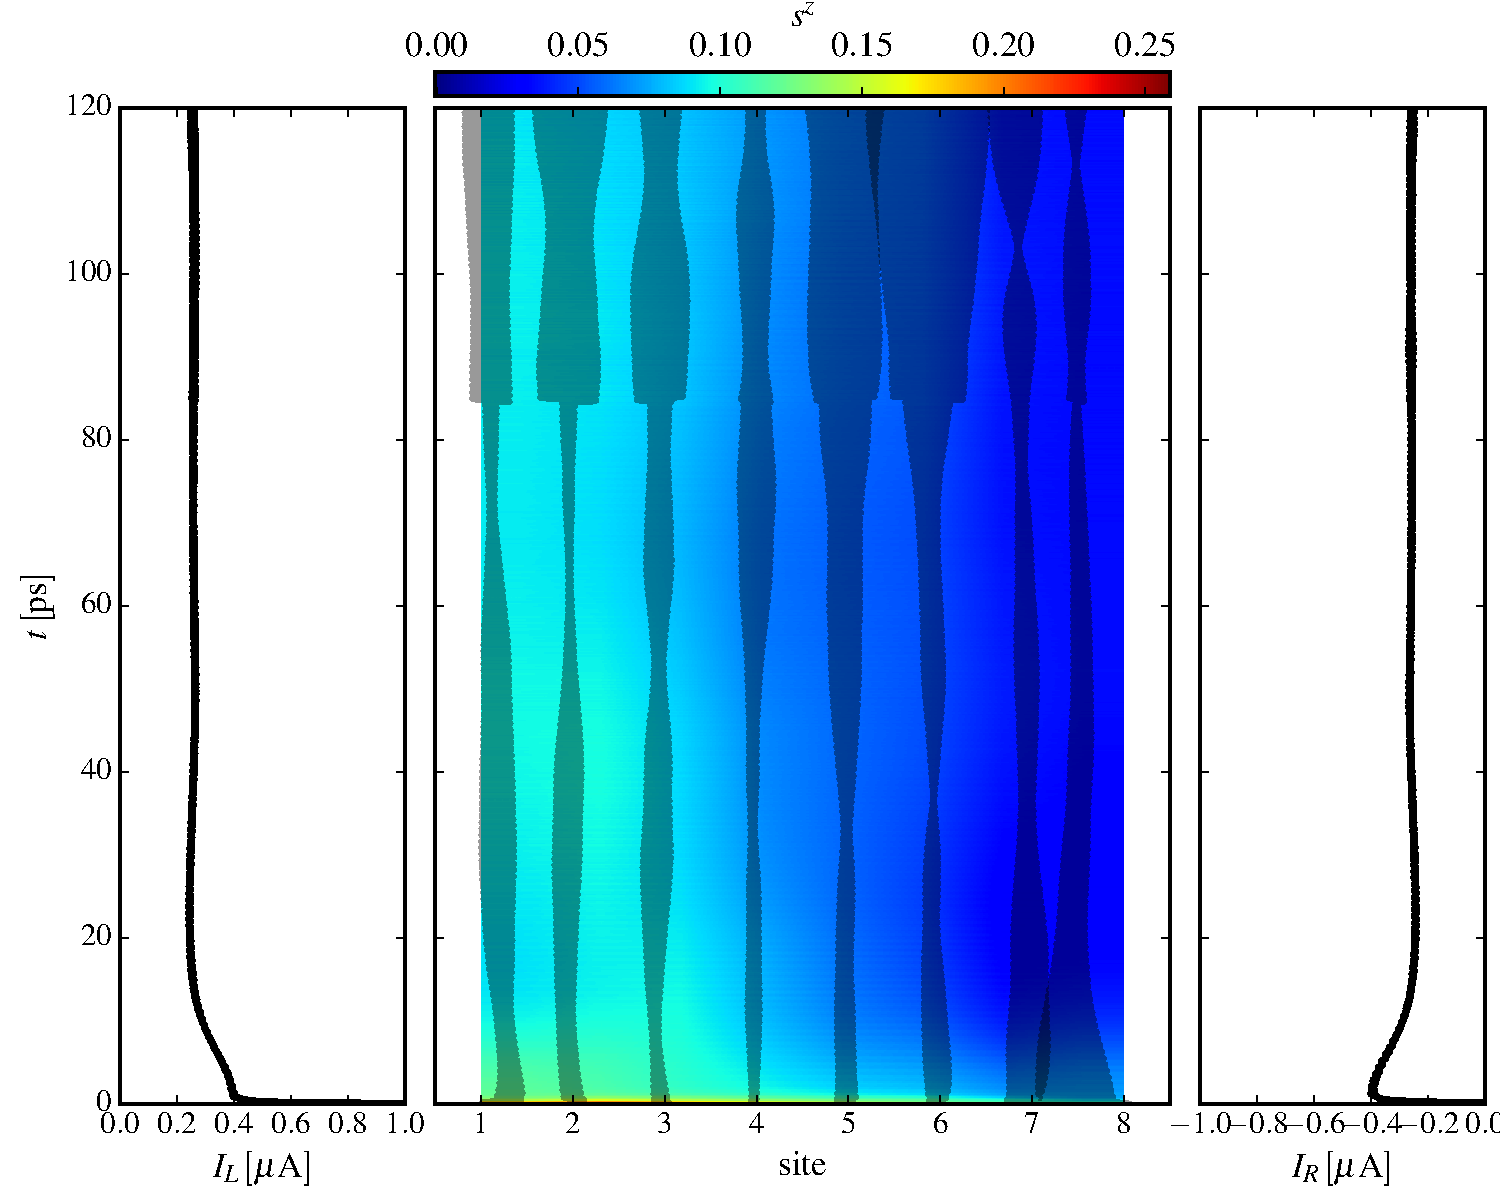
\includegraphics[width=0.8\textwidth]{figs/tsoPh0.1/L8_V60_tPh0.004_tso0.001_tsoPh0.0001_P_spins_tend120_currents_phonons.pdf}
	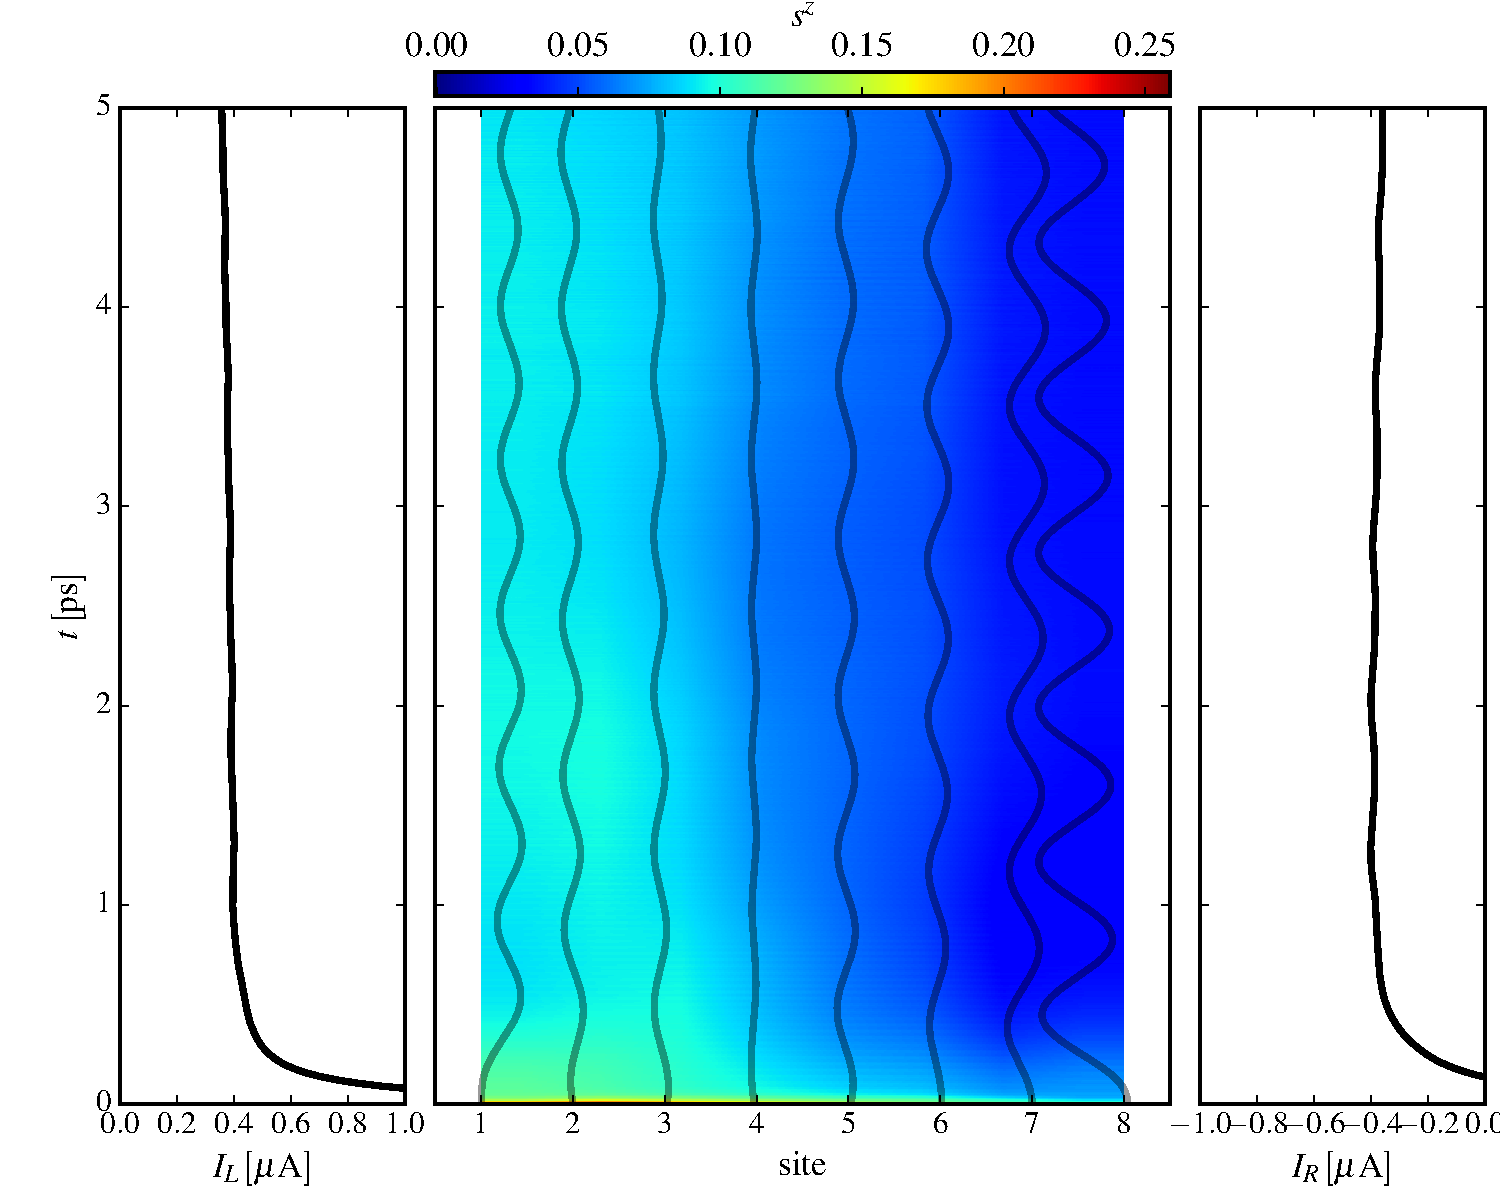
\includegraphics[width=0.8\textwidth]{figs/tsoPh0.1/L8_V60_tPh0.004_tso0.001_tsoPh0.0001_P_spins_tend5_currents_phonons.pdf}
	%~/PhD/projects/CISS_data/v2/I_V/w0_2_t1_4_tso_1_tsoPh_0.1/PVar/L2x4/v3/
	\caption{For $V=\SI{0.48}{\volt}$, $P=0.5$.}
\end{figure}



\clearpage

\subsection{$L=2\times 4$, $\lambda_0=\SI{10}{\milli\electronvolt}$, $\lambda_1=\SI{0.1}{\milli\electronvolt}$}
\subsubsection{Time-dependent electronic spectrum and voltage regimes}
\begin{figure}[!h]
	\centering
	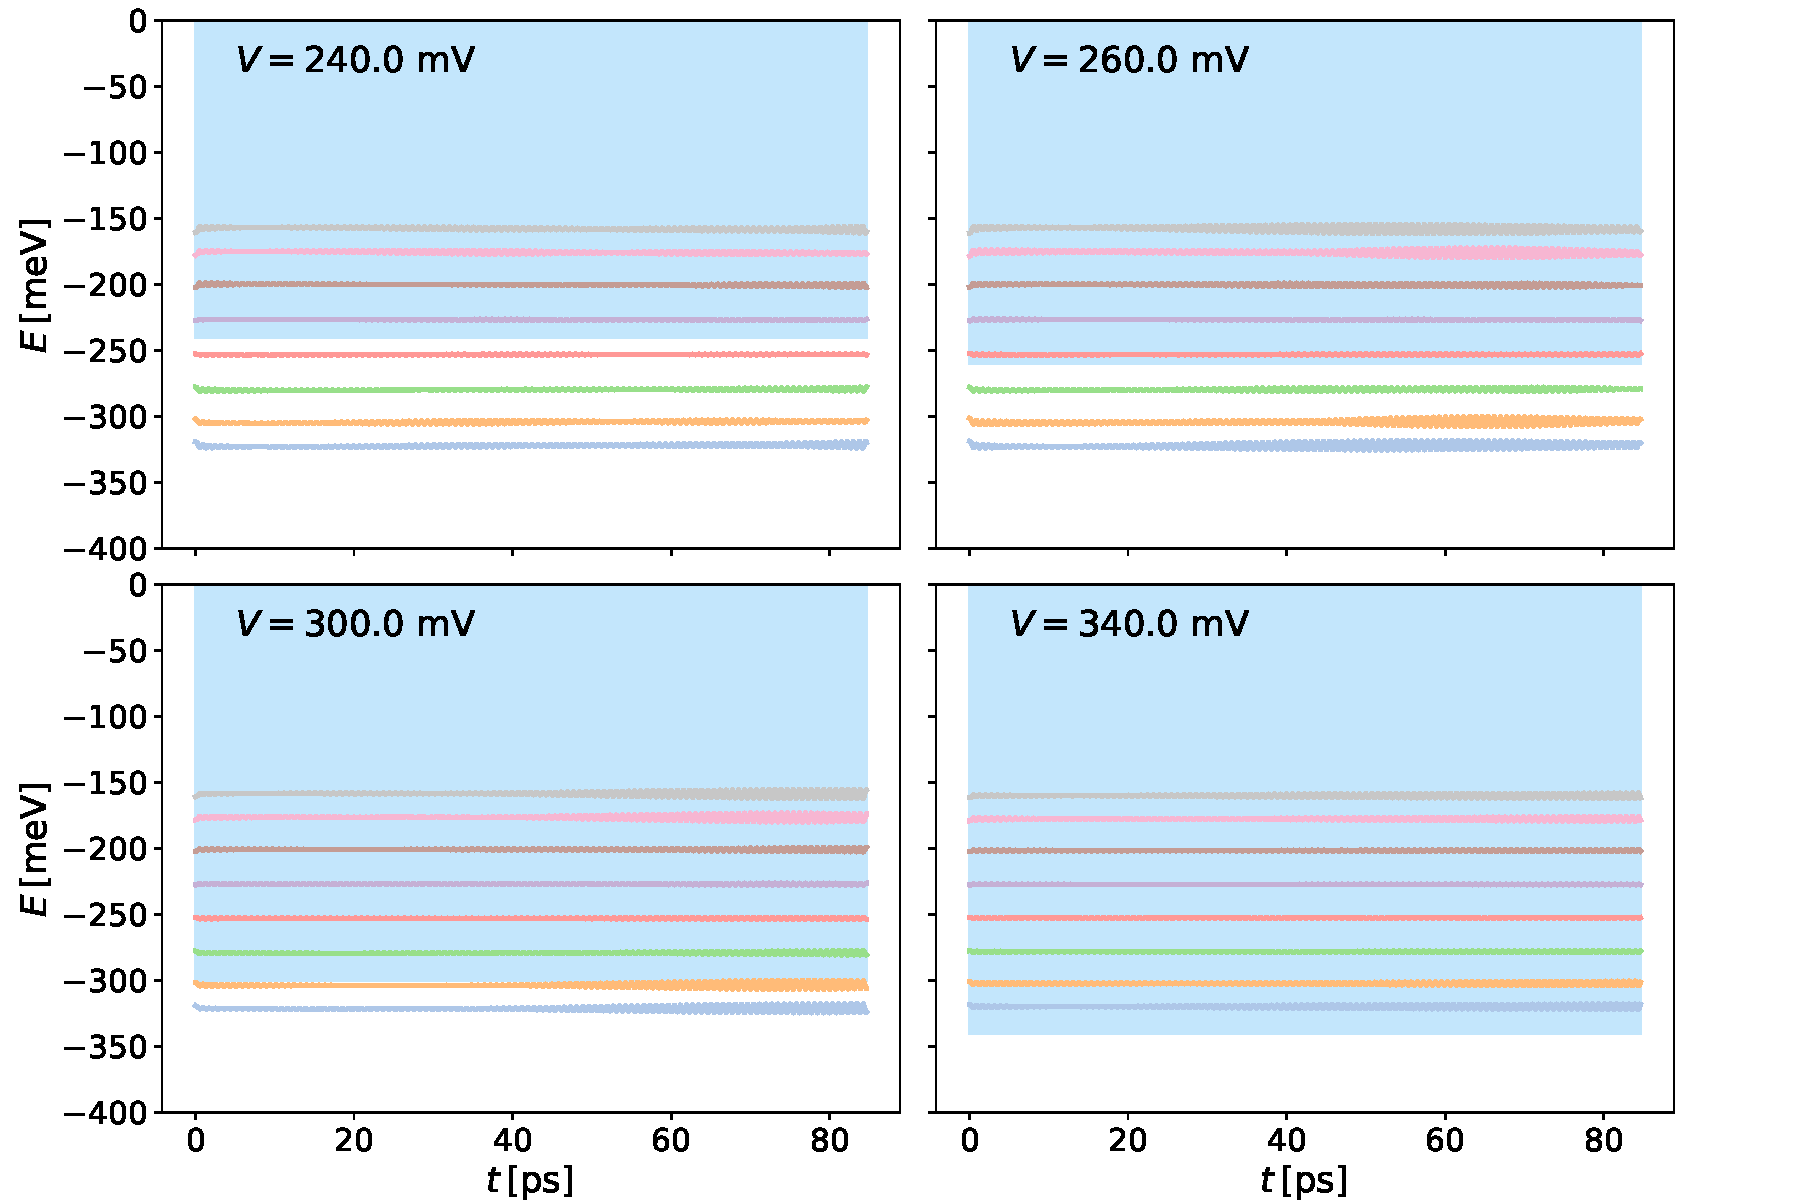
\includegraphics[width=0.9\textwidth]{figs/tso10_tsoPh0.1/L2x4_spectrumTD_PhAvg_tso5.0_tsoPh0.01.pdf}
	% ~/PhD/projects/CISS_data/v2/I_V/w0_2_t1_4_tso_10_tsoPh_0.1/L2x4/v1
\end{figure}
\clearpage
\subsubsection{Time-dependent charge currents and spin selectivity}
\begin{figure}[!h]
	\centering
	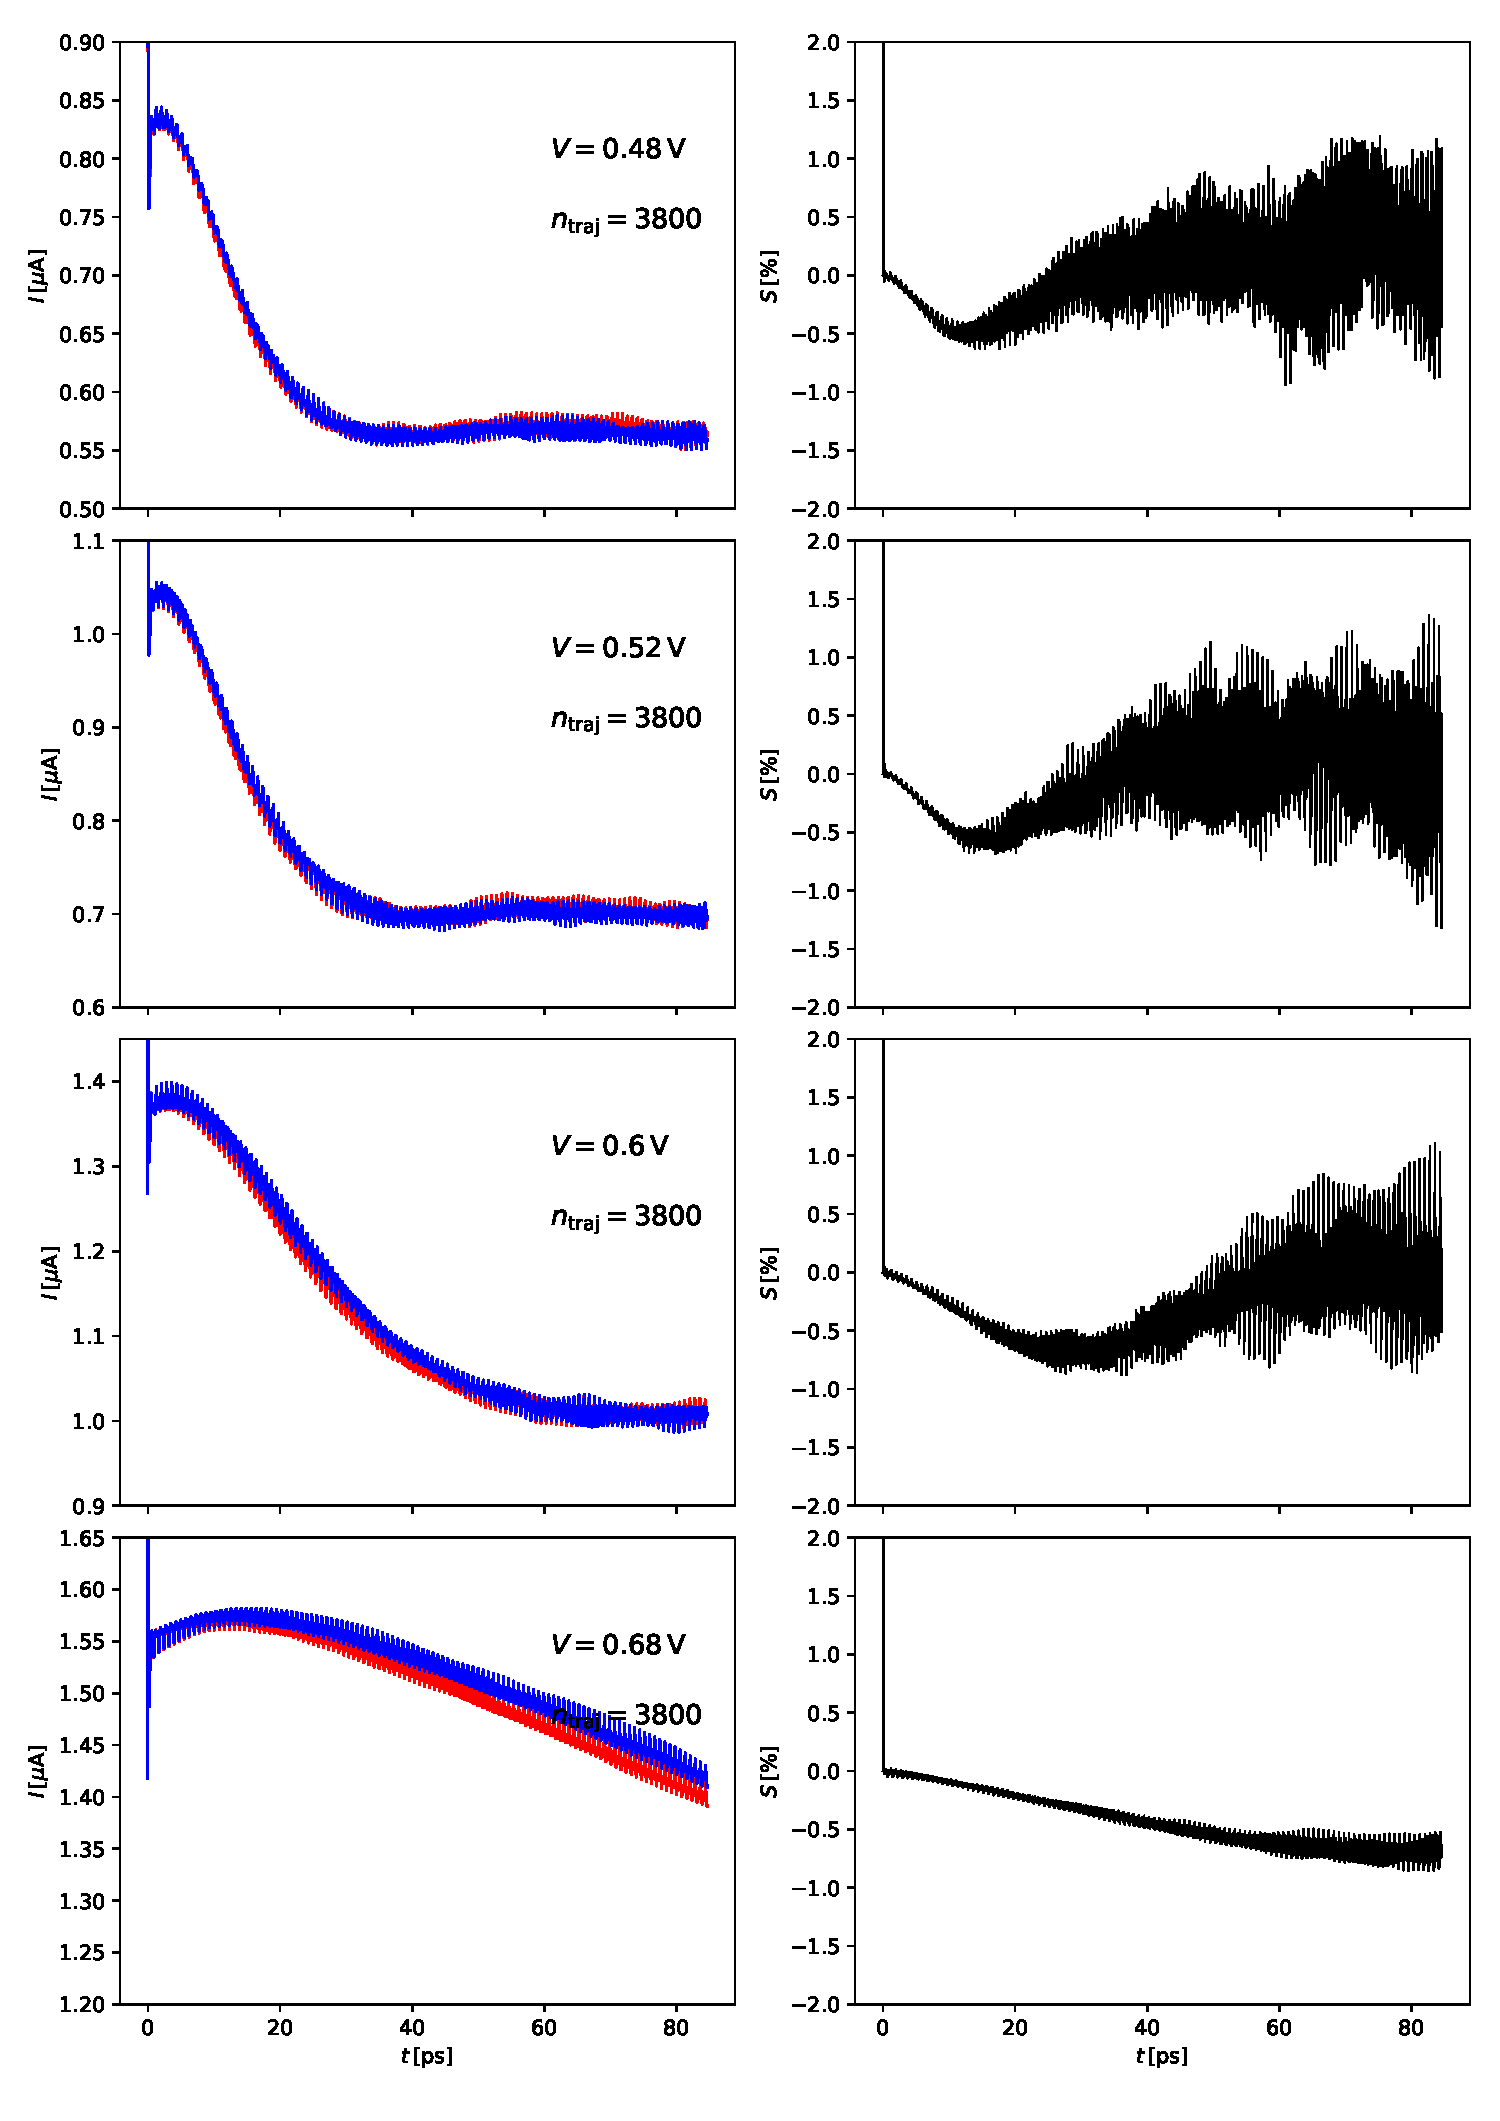
\includegraphics[width=0.9\textwidth]{figs/tso10_tsoPh0.1/L2x4_currents_MR_allV_tso10_tsoPh0.1.pdf}
	% ~/PhD/projects/CISS_data/v2/I_V/w0_2_t1_4_tso_10_tsoPh_0.1/L2x4/v1
\end{figure}
\clearpage
\subsubsection{Time-dependent charge currents and spin selectivity with IIR filtering}
\begin{figure}[!h]
	\centering
	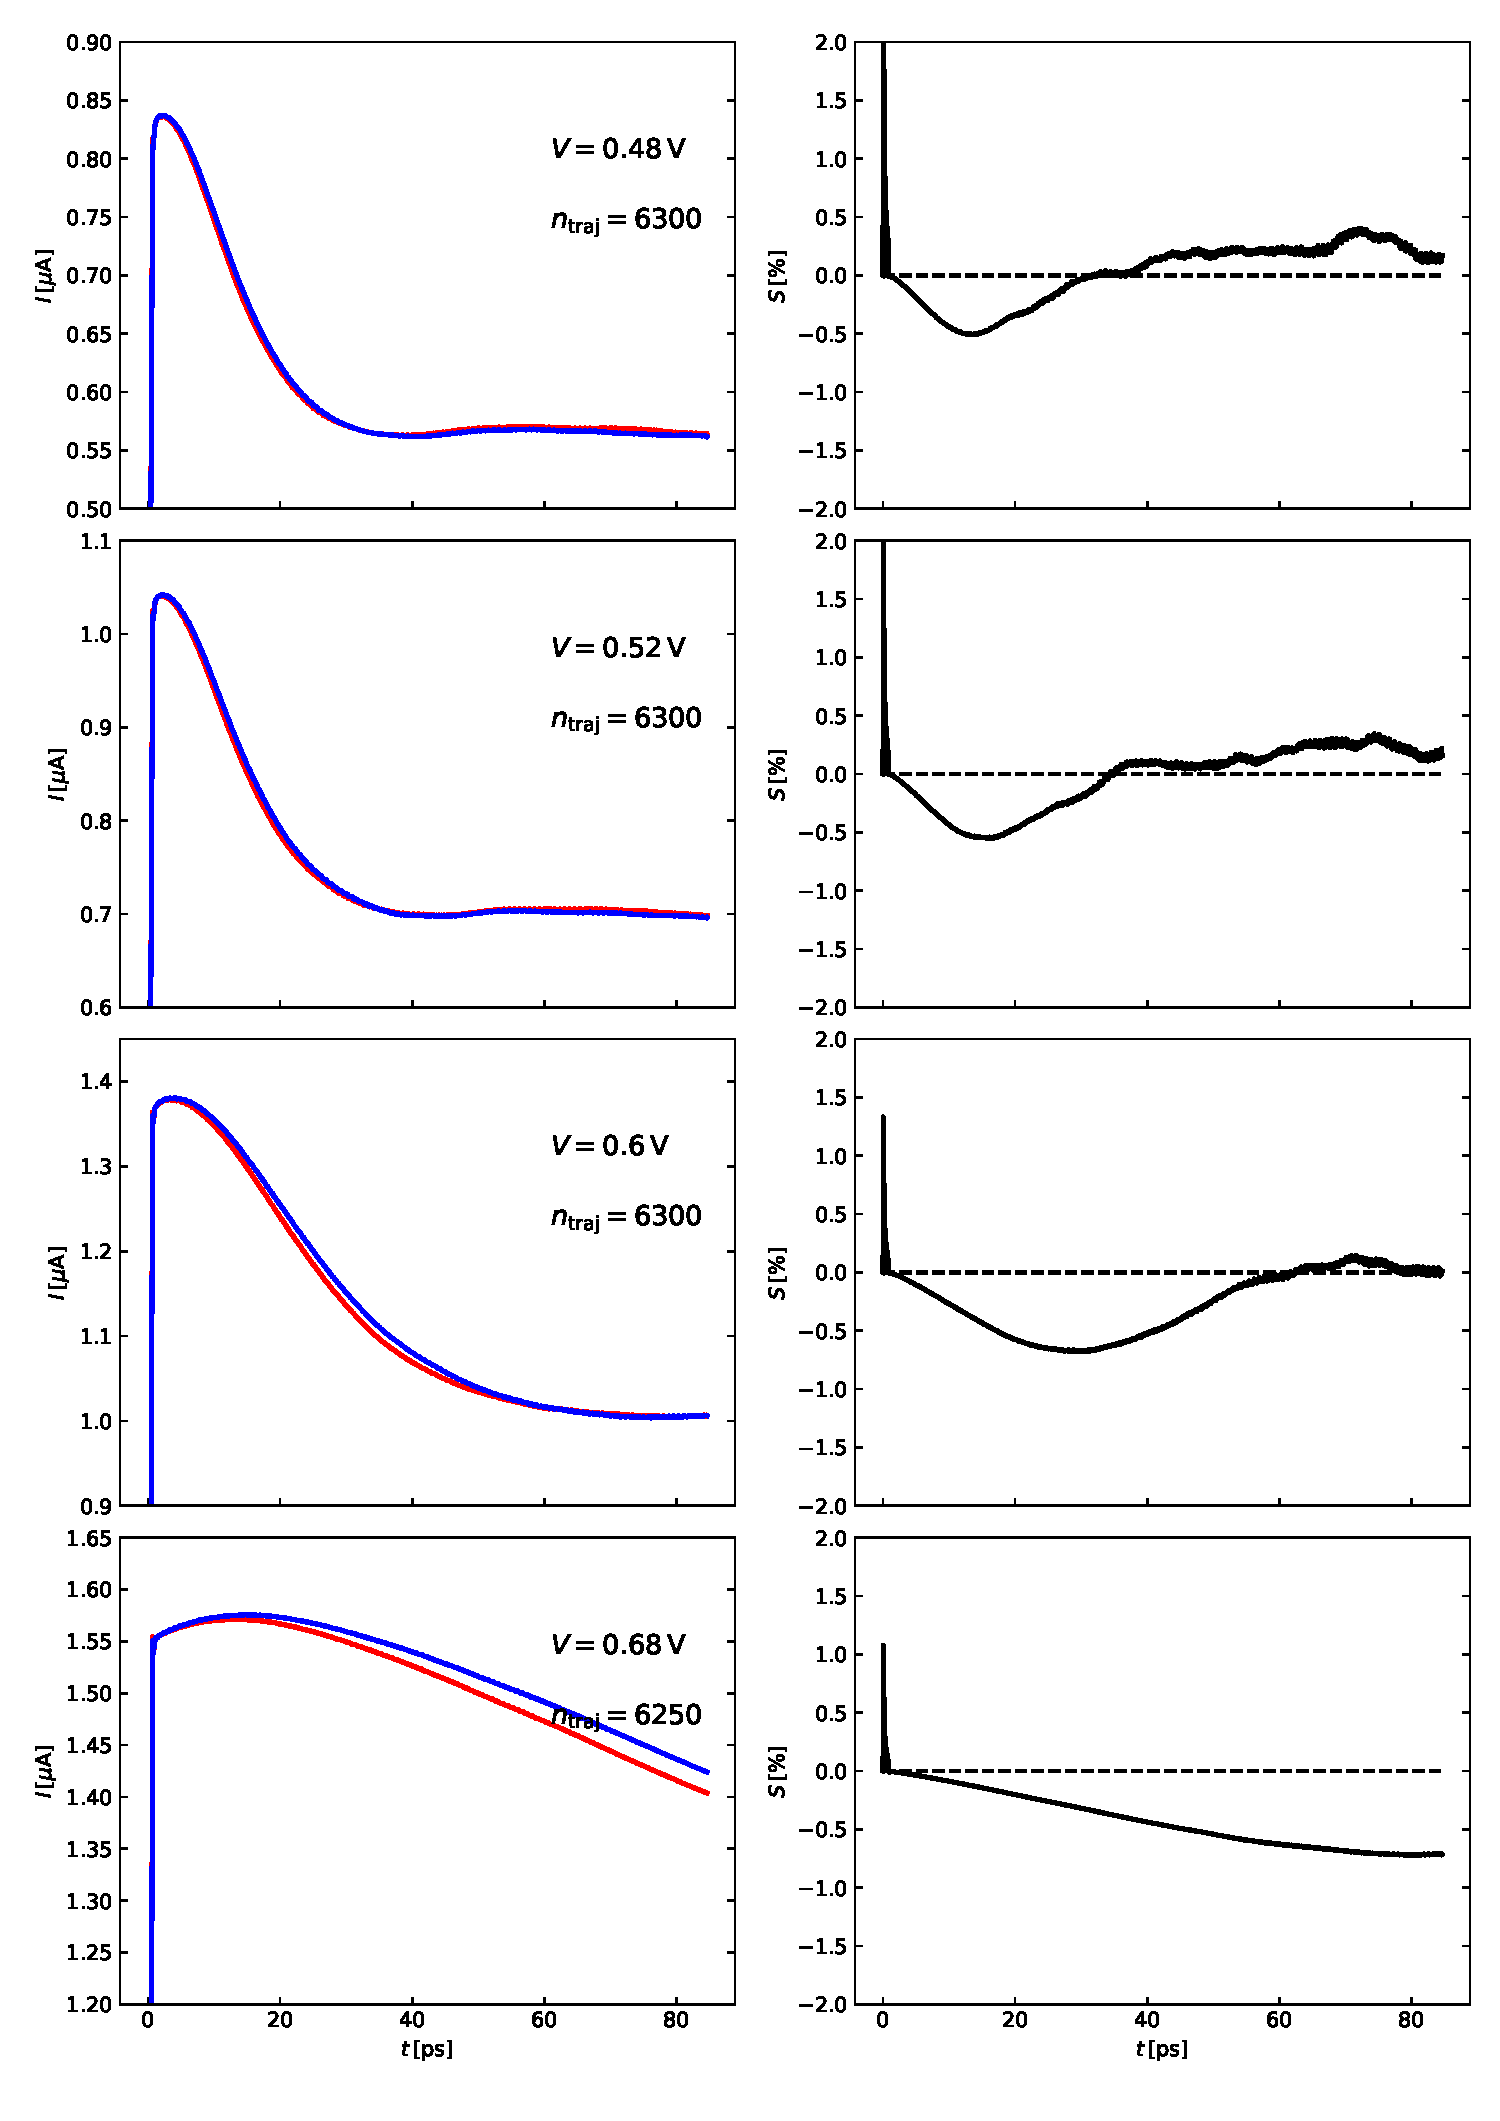
\includegraphics[width=0.9\textwidth]{figs/tso10_tsoPh0.1/L2x4_currents_MR_allV_tso10_tsoPh0.1_filtered.pdf}
	% ~/PhD/projects/CISS_data/v2/I_V/w0_2_t1_4_tso_10_tsoPh_0.1/L2x4/v1
\end{figure}
\clearpage

\subsection{$L=2\times 4$, $\lambda_0=\SI{1}{\milli\electronvolt}$, $\lambda_1=\SI{5}{\milli\electronvolt}$}
\begin{figure}[!h]
	\centering
	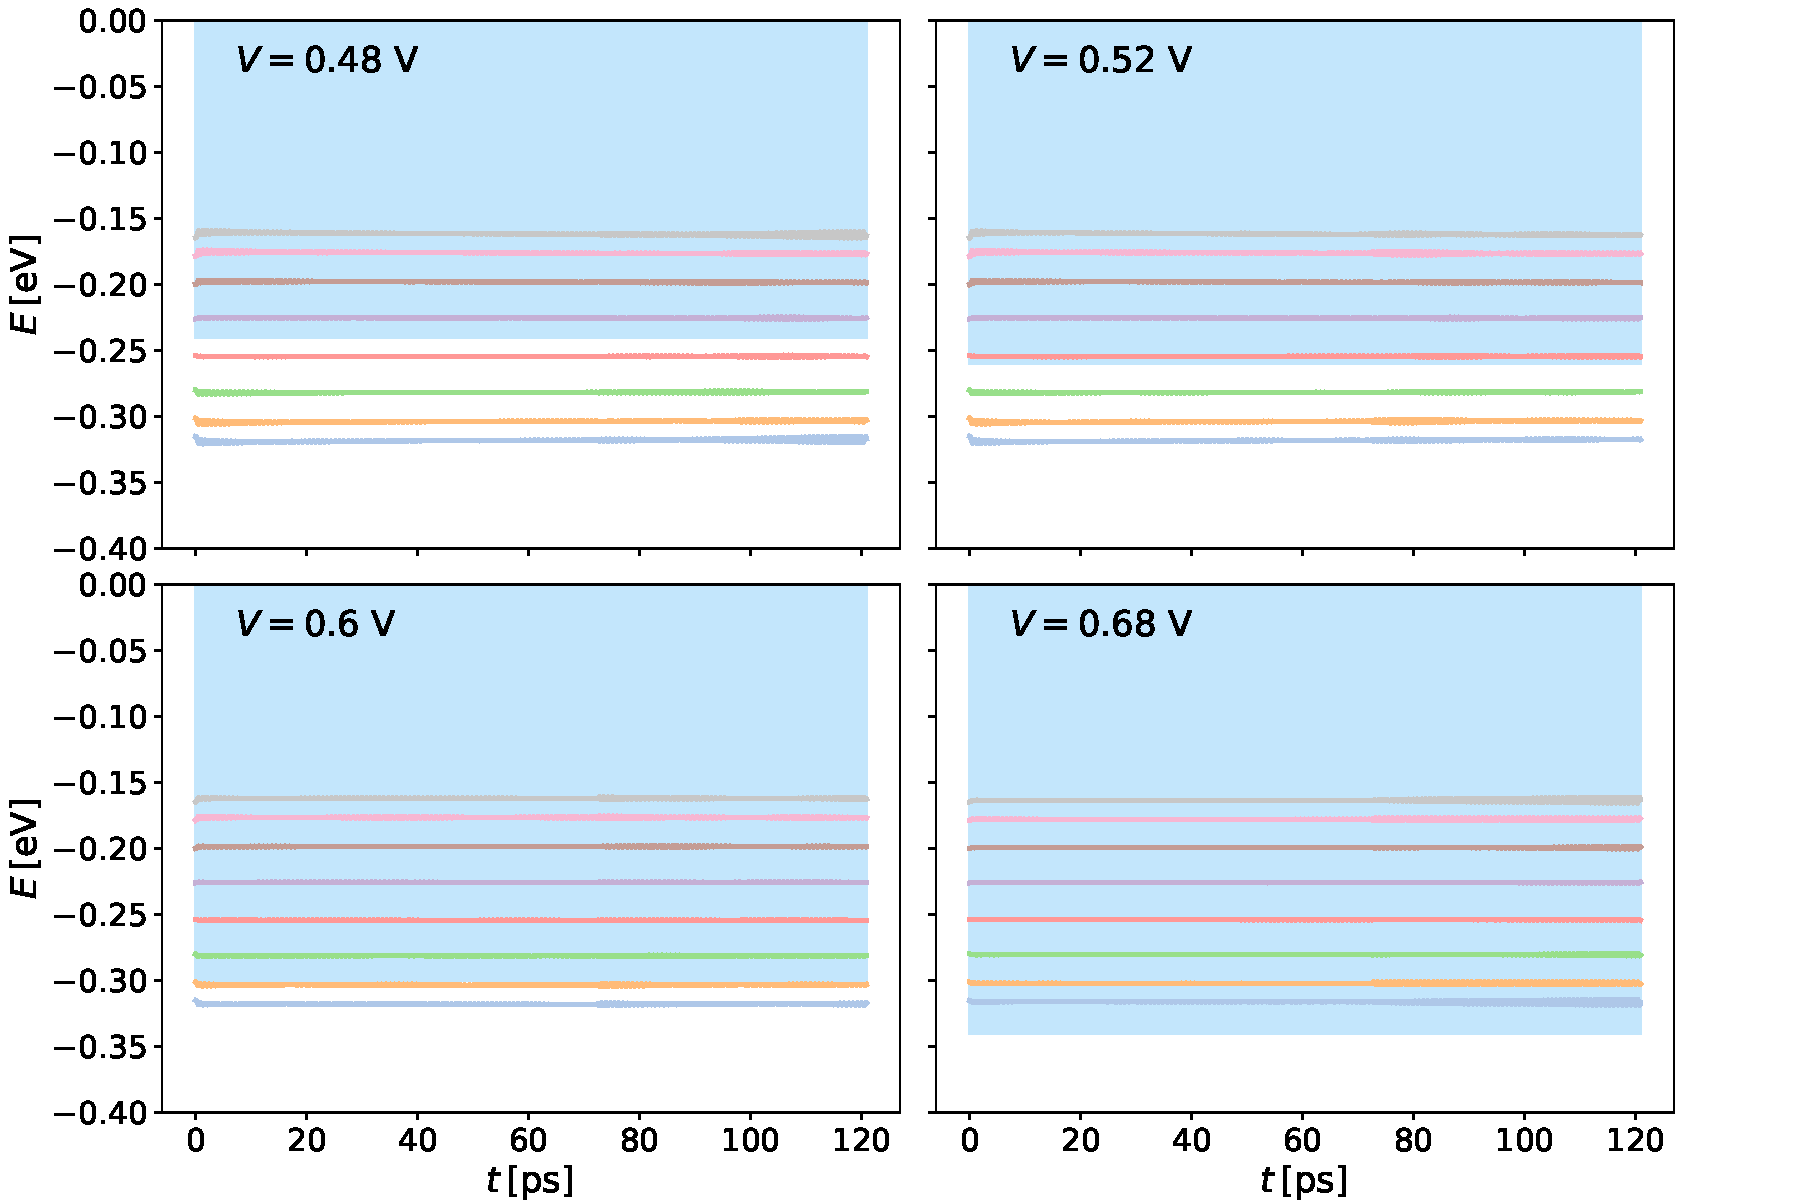
\includegraphics[width=0.9\textwidth]{figs/tsoPh5/L2x4_spectrumTD_PhAvg_tso0.5_tsoPh5.0.pdf}
	%~/PhD/projects/CISS_data/v2/I_V/w0_2_t1_4_tso_1_tsoPh_5/L2x4/comb
\end{figure}
\begin{figure}[!h]
	\centering
	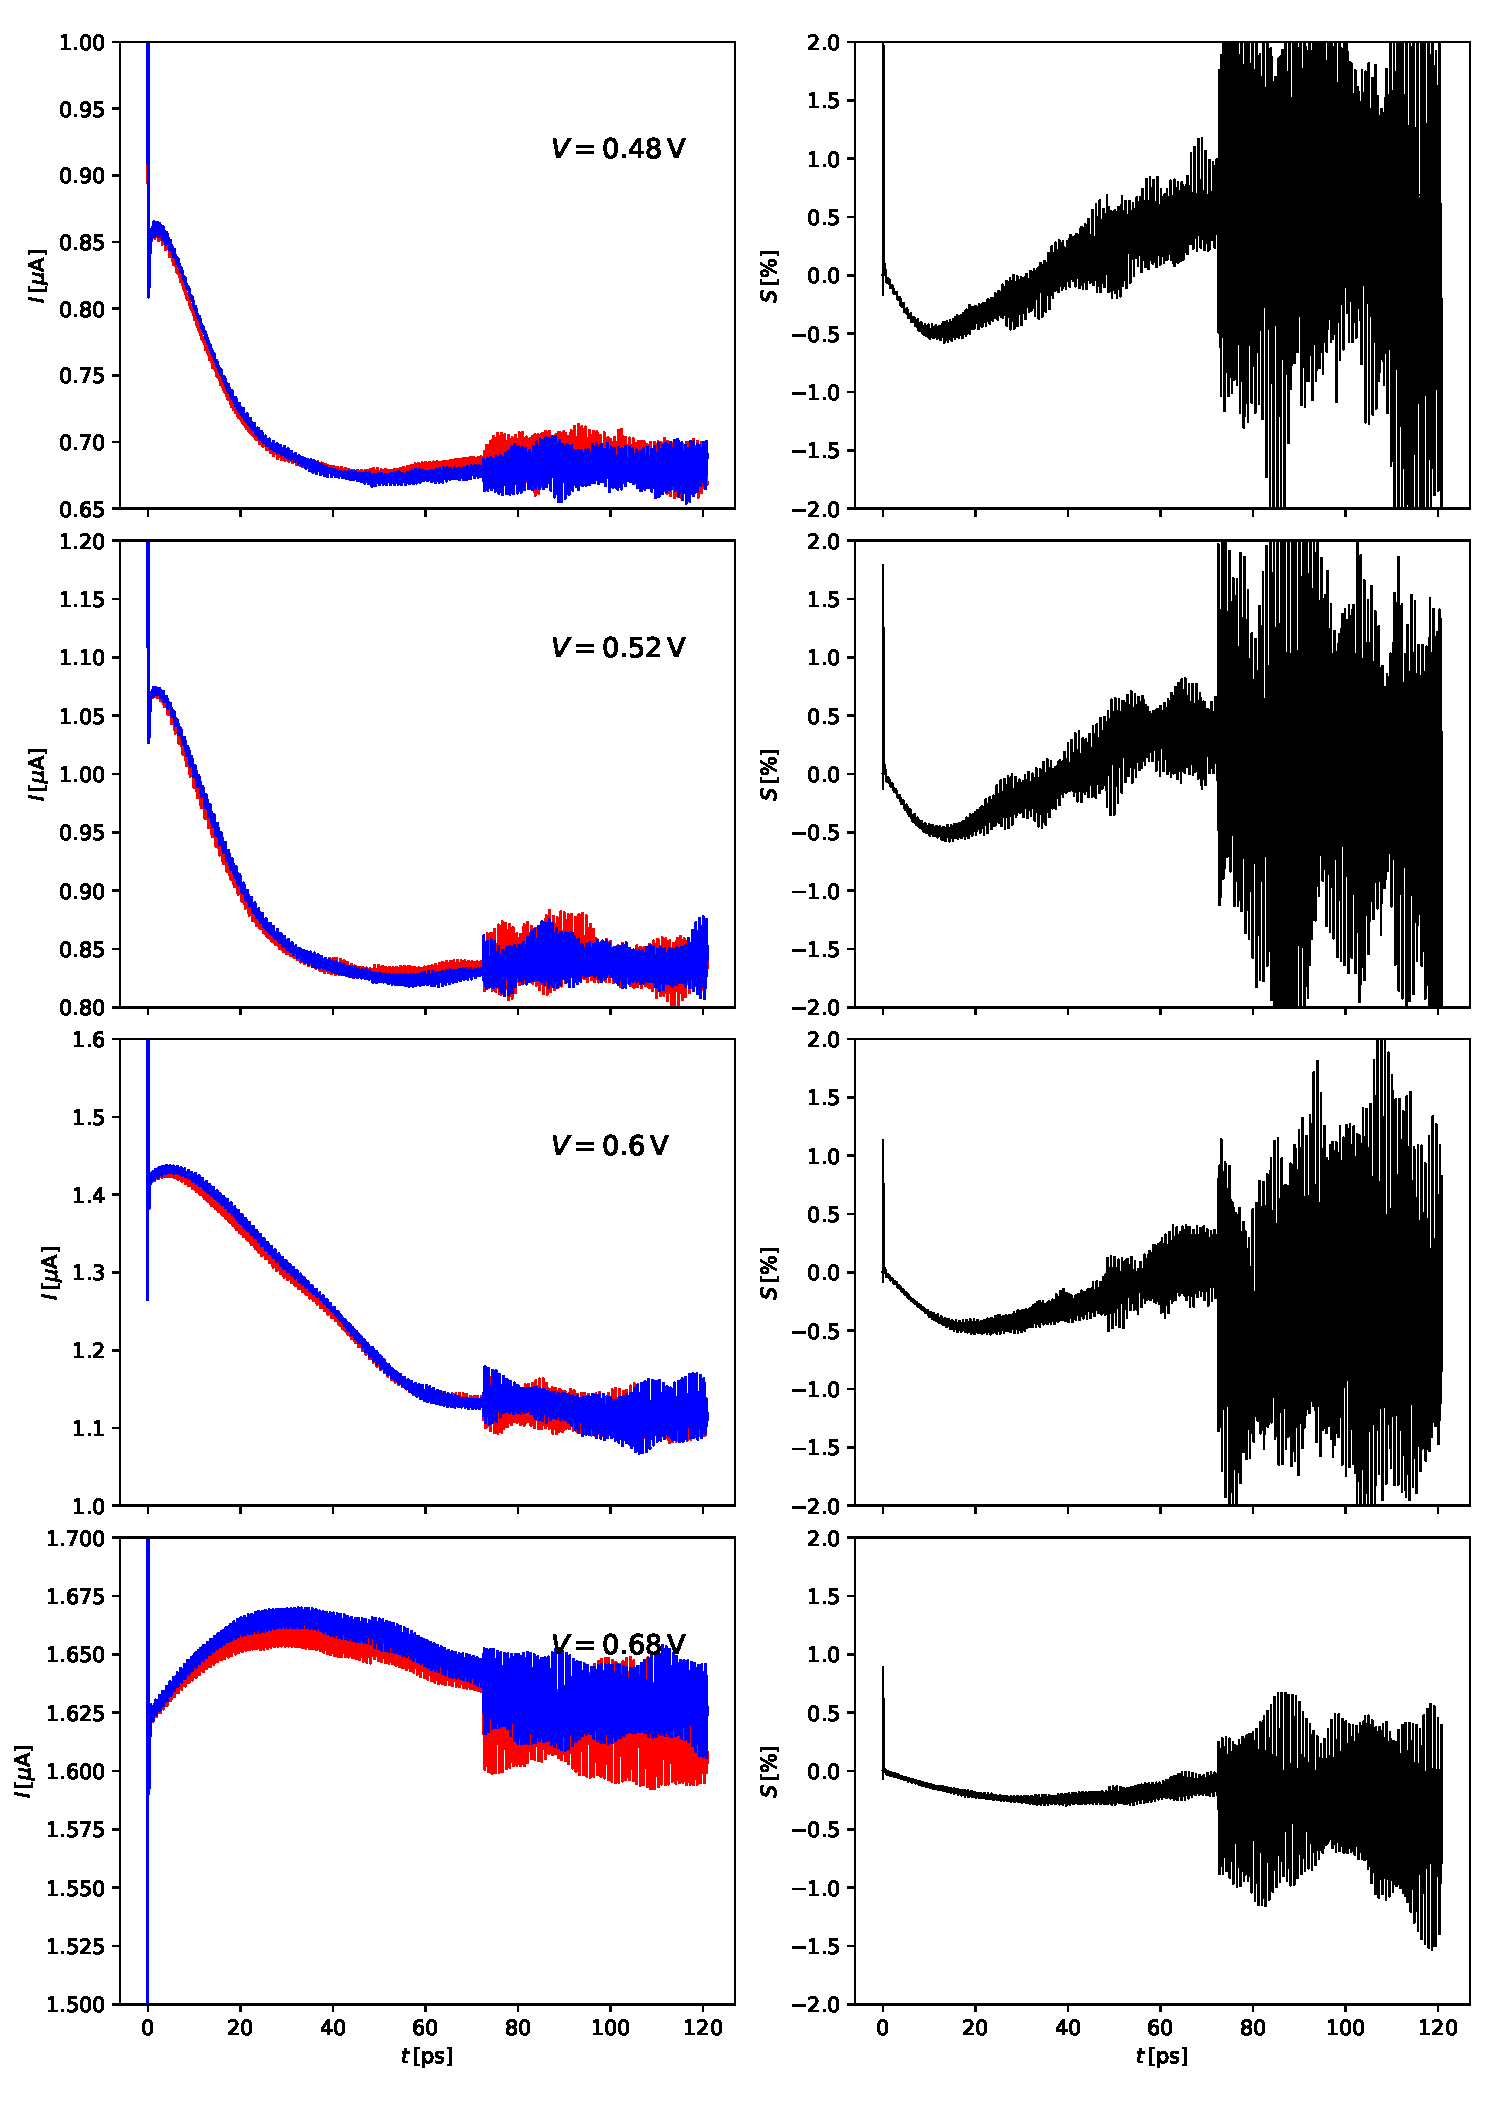
\includegraphics[width=0.9\textwidth]{figs/tsoPh5/L2x4_currents_MR_allV_tsoPh5.pdf}
	%~/PhD/projects/CISS_data/v2/I_V/w0_2_t1_4_tso_1_tsoPh_5/L2x4/comb
\end{figure}
\clearpage
\subsection{$L=2\times 4$, $\lambda_0=\SI{1}{\milli\electronvolt}$, $\lambda_1=\SI{10}{\milli\electronvolt}$}
\begin{figure}[!h]
	\centering
	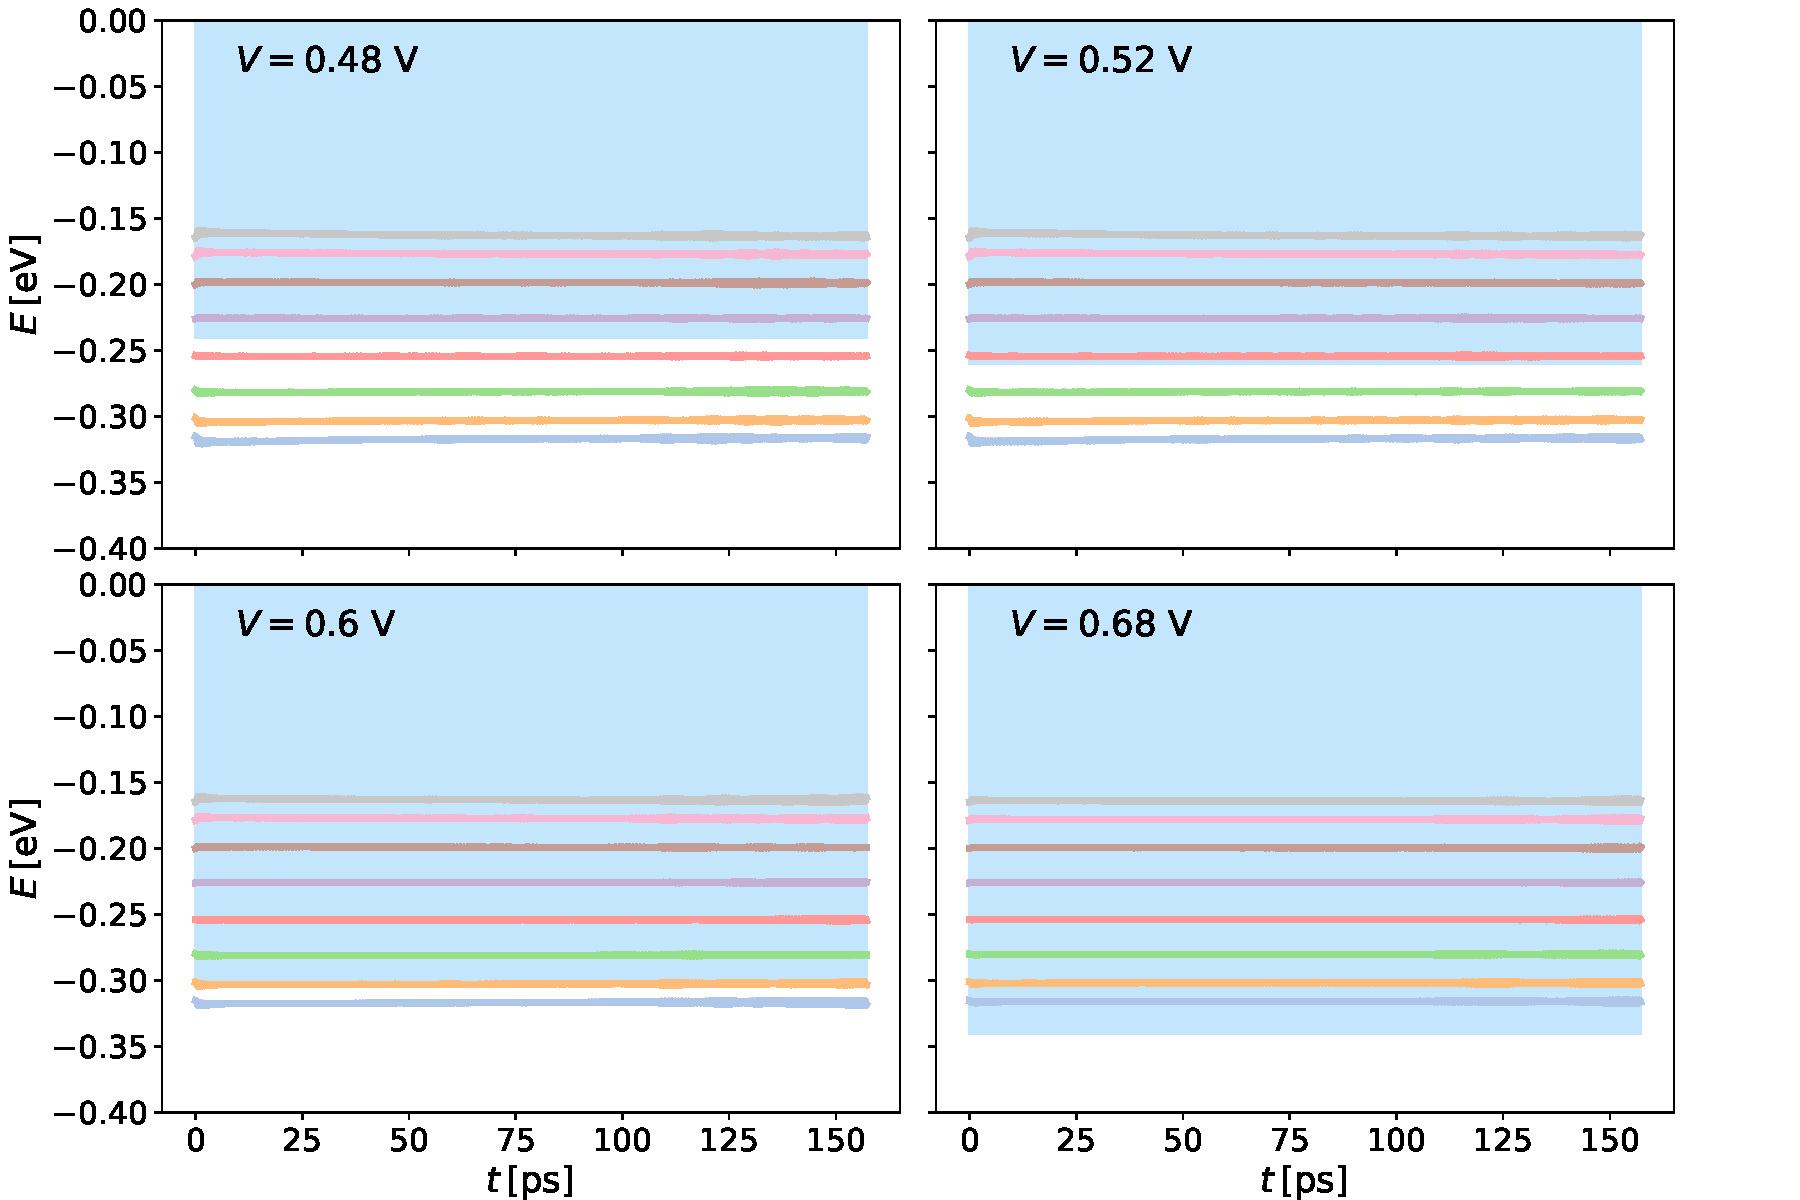
\includegraphics[width=0.9\textwidth]{figs/tsoPh10/L2x4_spectrumTD_PhAvg_tsoPh10.0.pdf}
\end{figure}
\begin{figure}[!h]
	\centering
	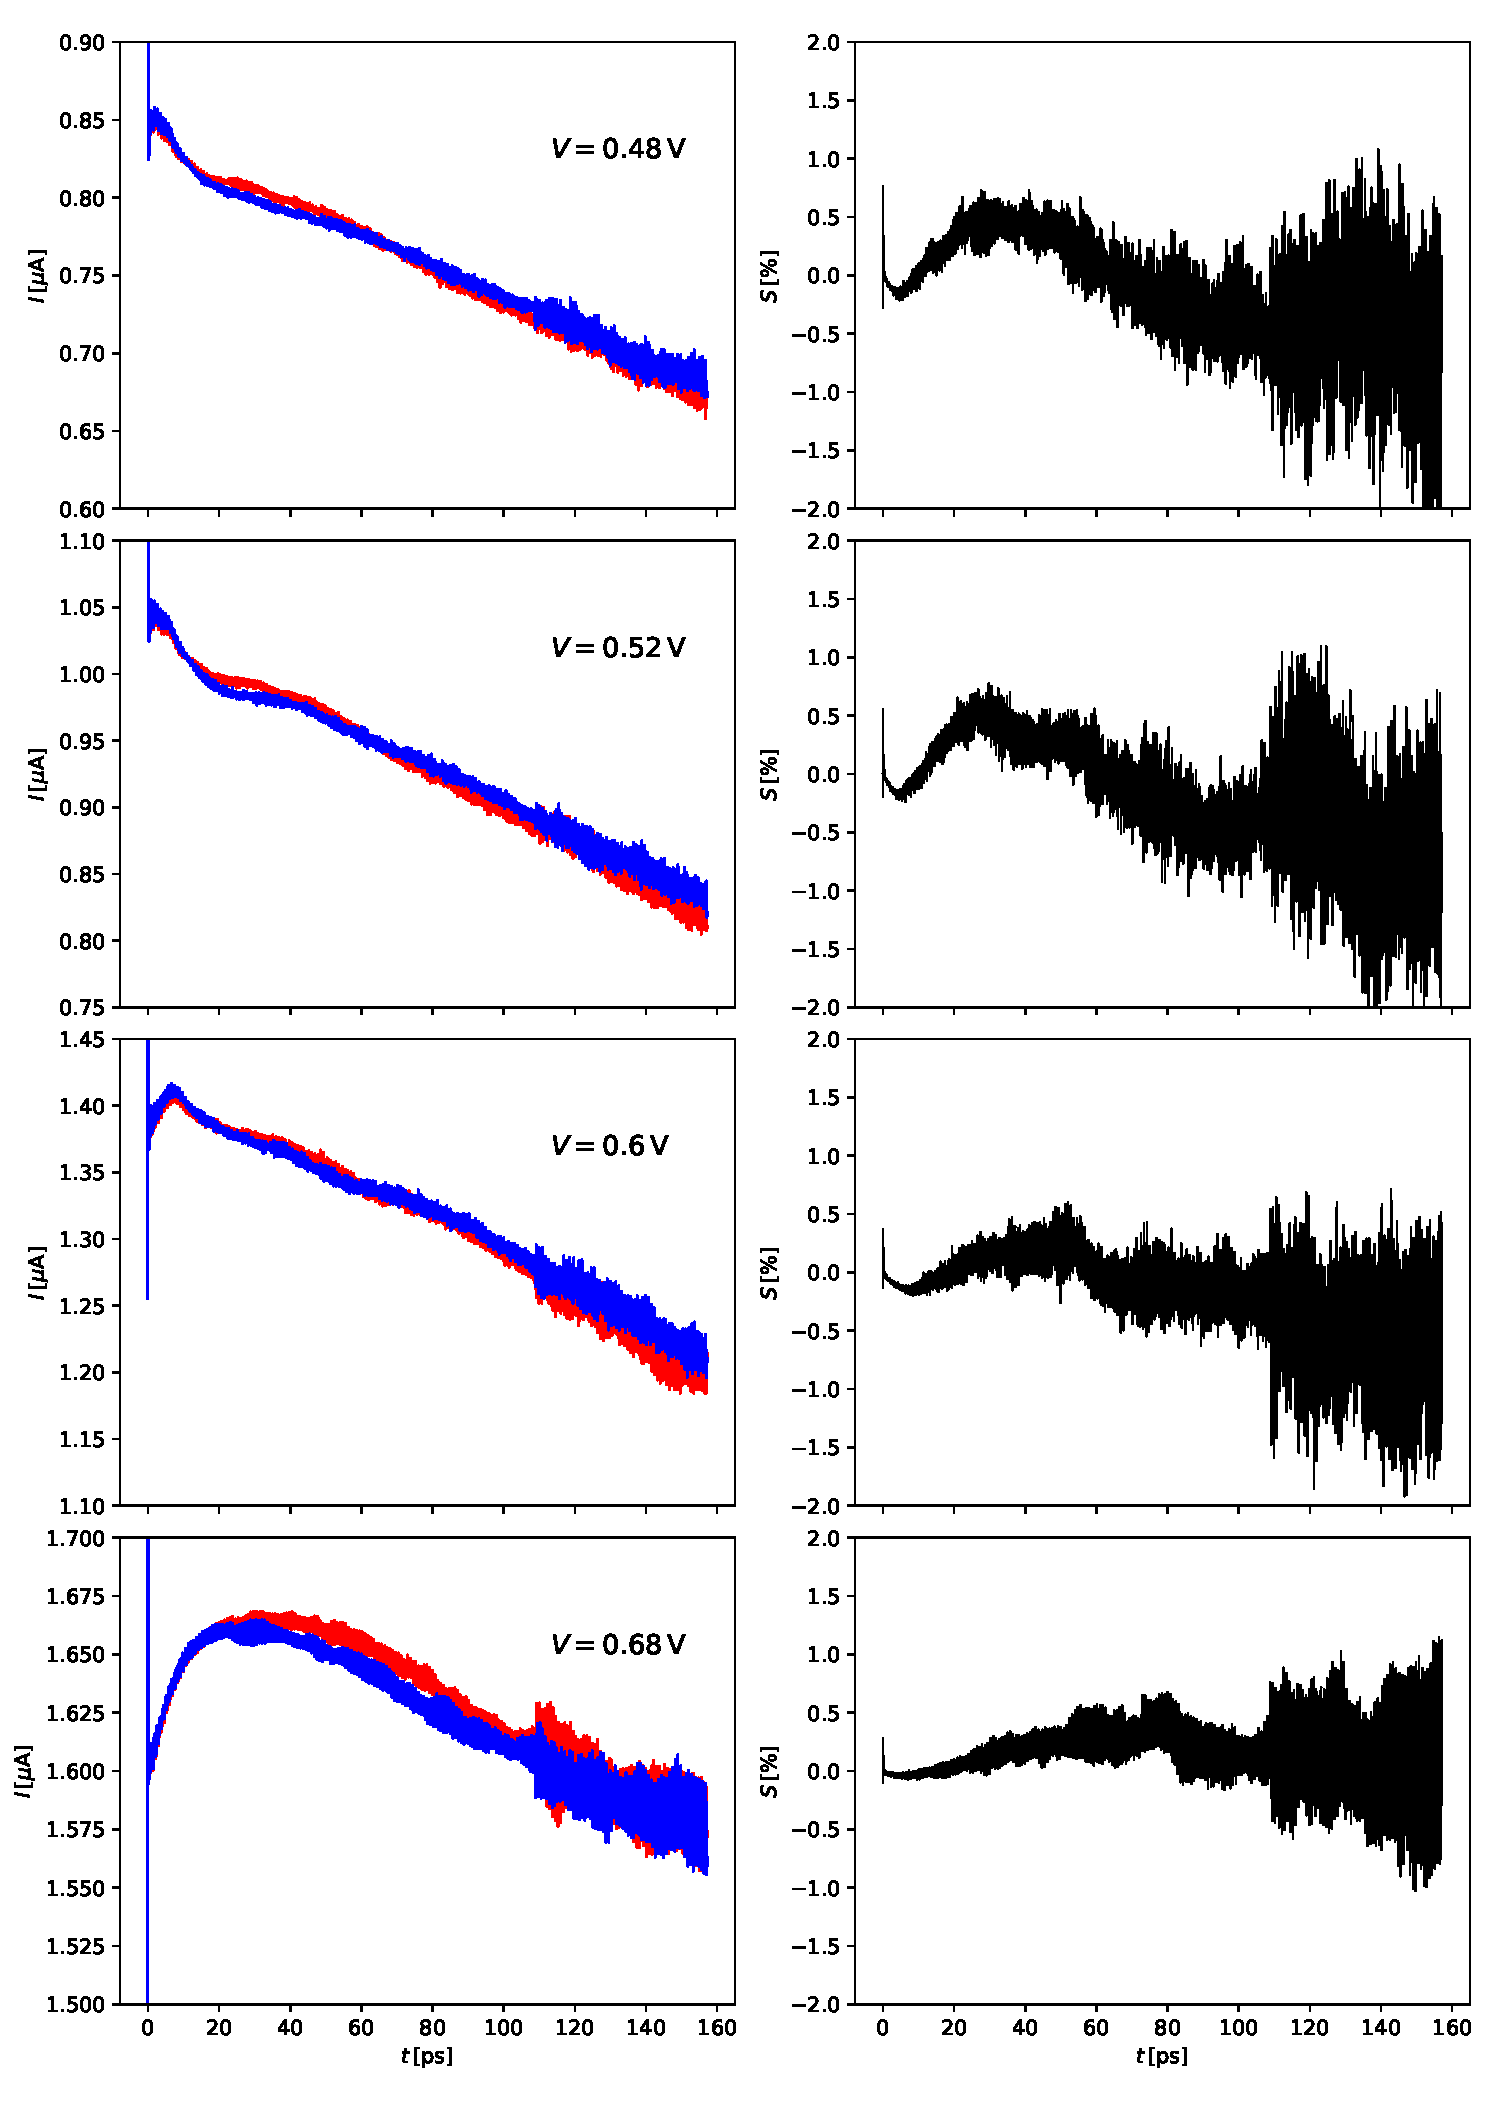
\includegraphics[width=0.9\textwidth]{figs/tsoPh10/L2x4_currents_MR_allV_tsoPh10.pdf}
\end{figure}
\begin{figure}[!h]
	\centering
	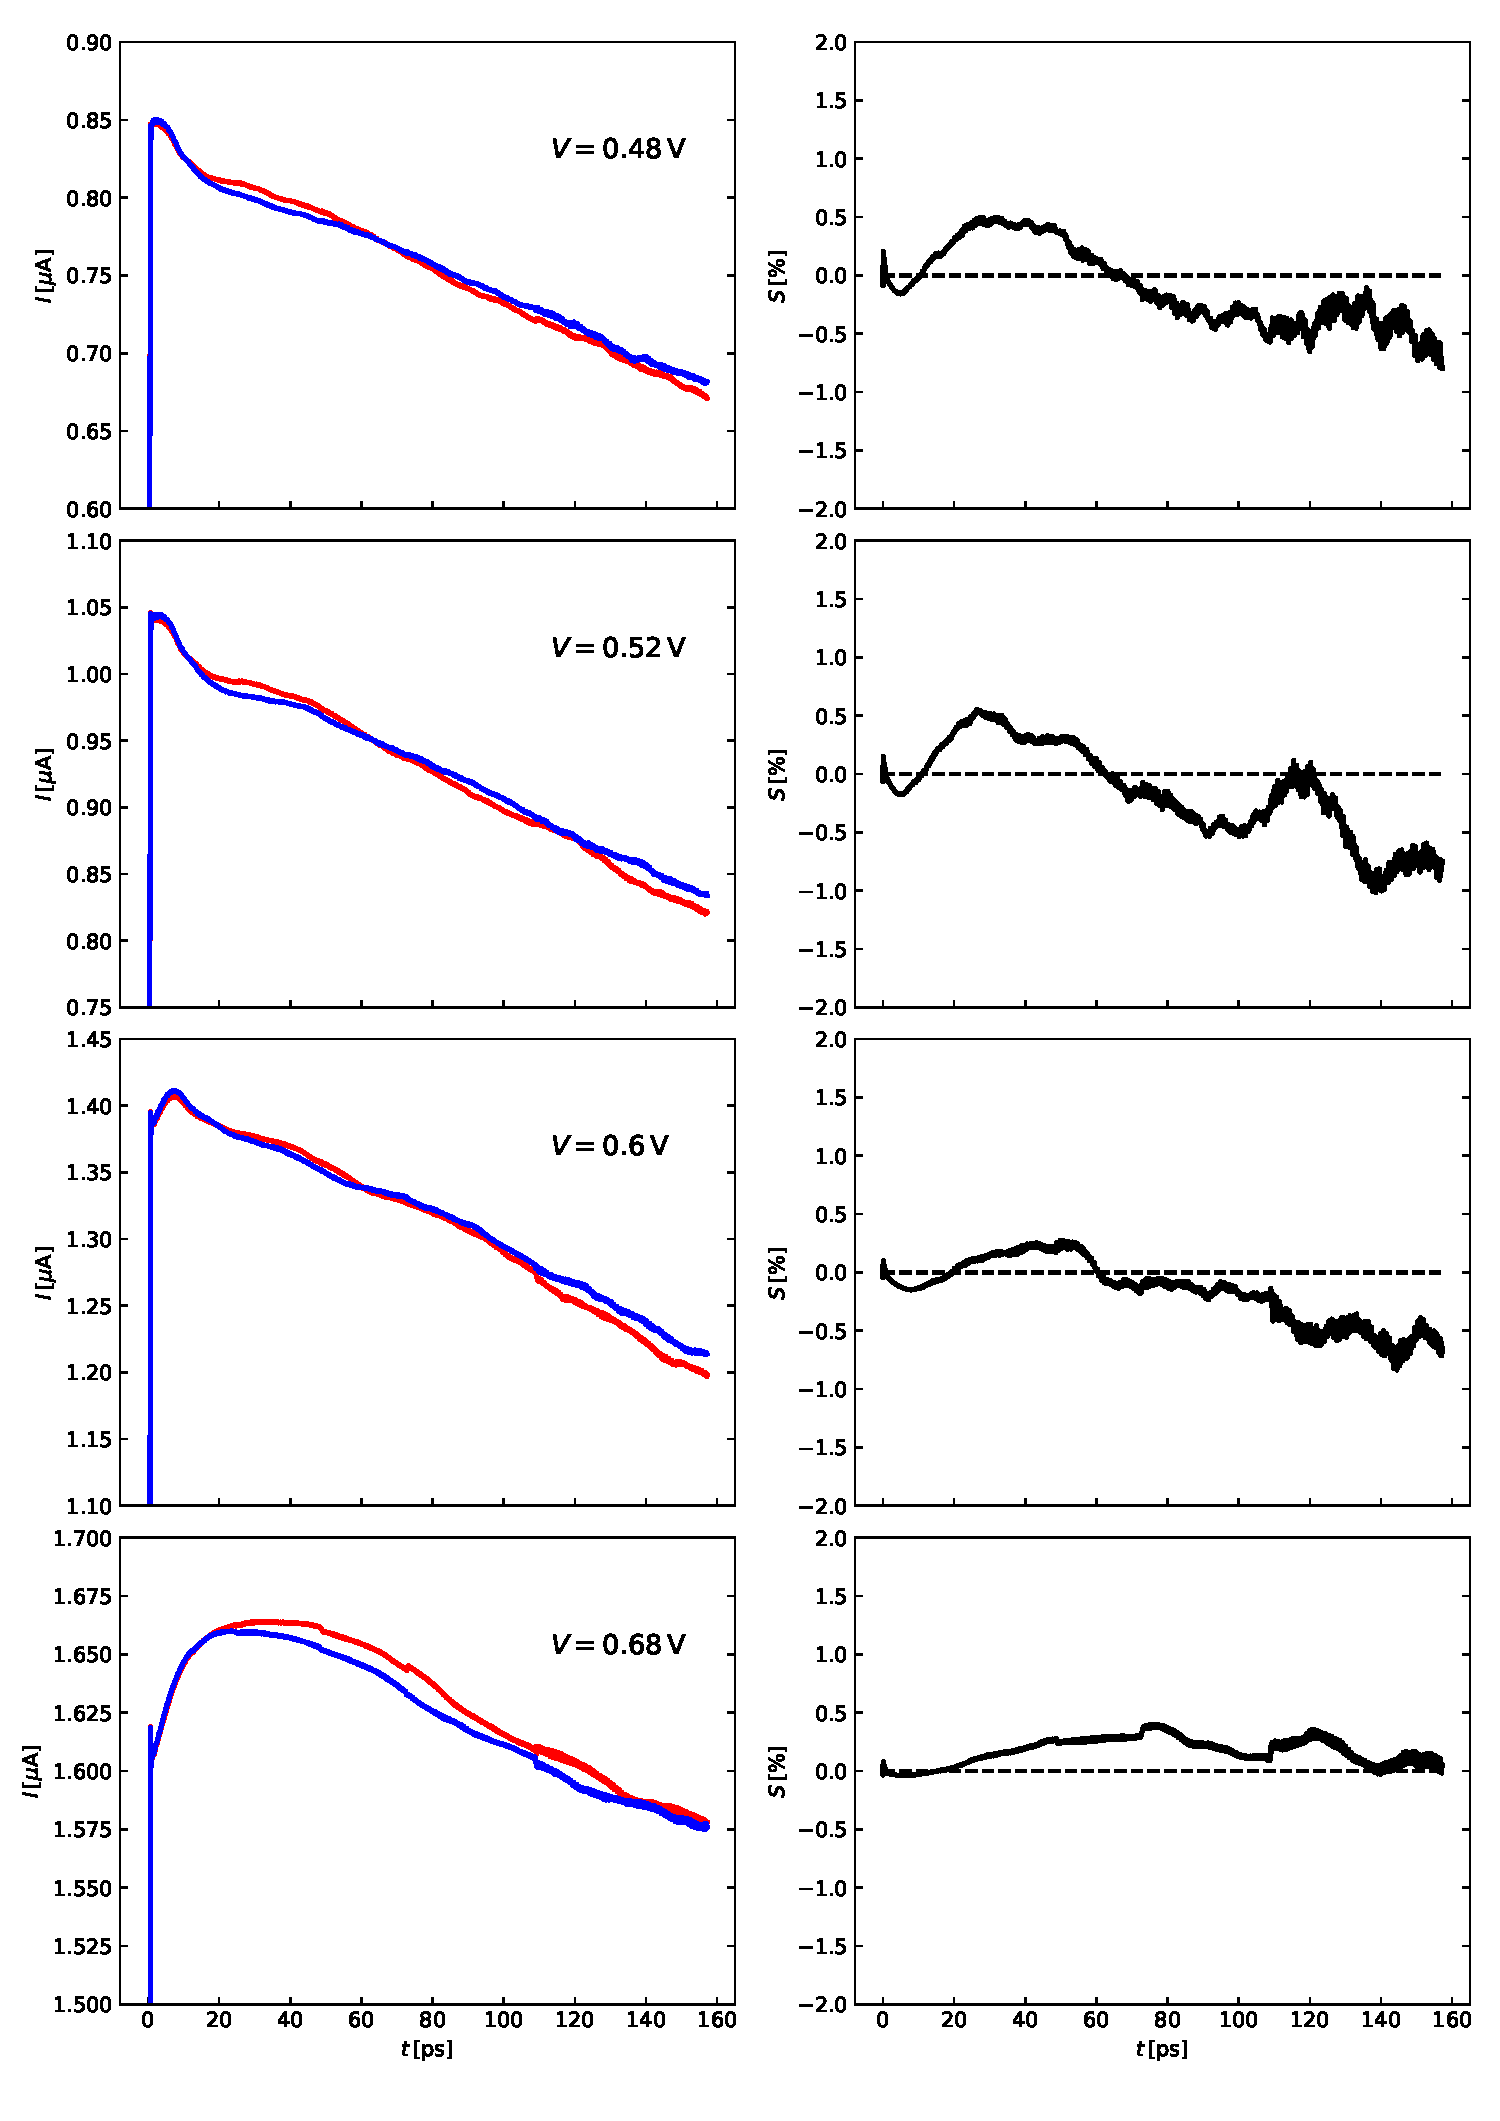
\includegraphics[width=0.9\textwidth]{figs/tsoPh10/L2x4_currents_MR_allV_tsoPh10_filtered.pdf}
\end{figure}
\begin{figure}[!h]
	\centering
	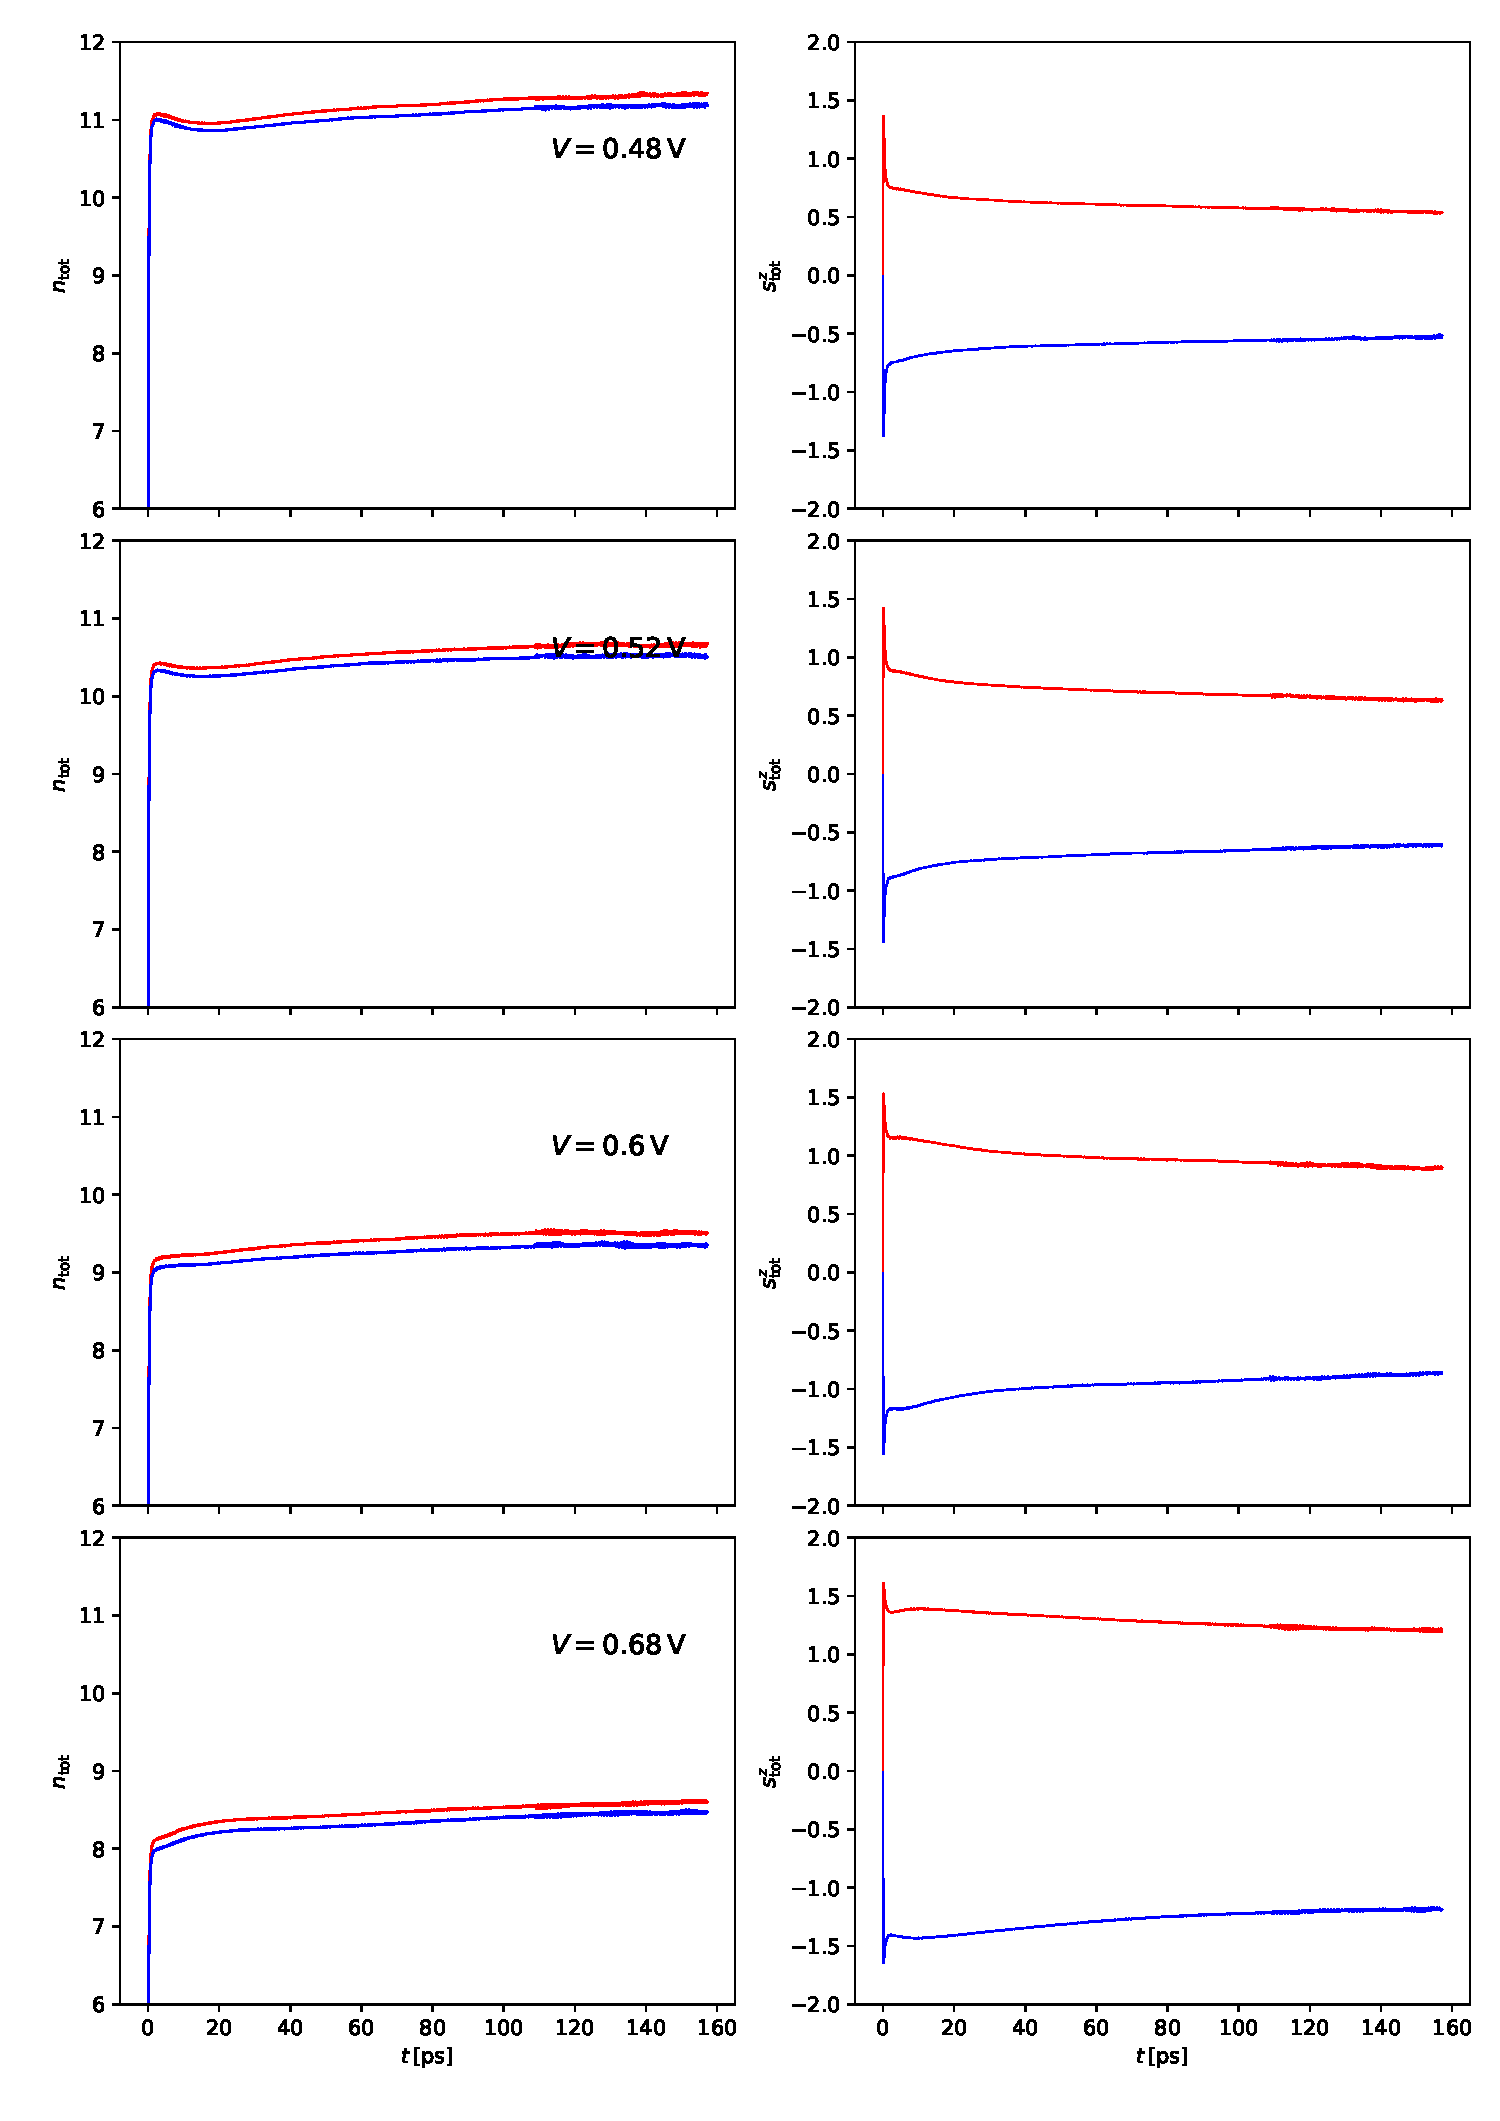
\includegraphics[width=0.9\textwidth]{figs/tsoPh10/L2x4_charge_sz_tot_allV_tsoPh10.pdf}
\end{figure}
\begin{figure}[!h]
	\centering
	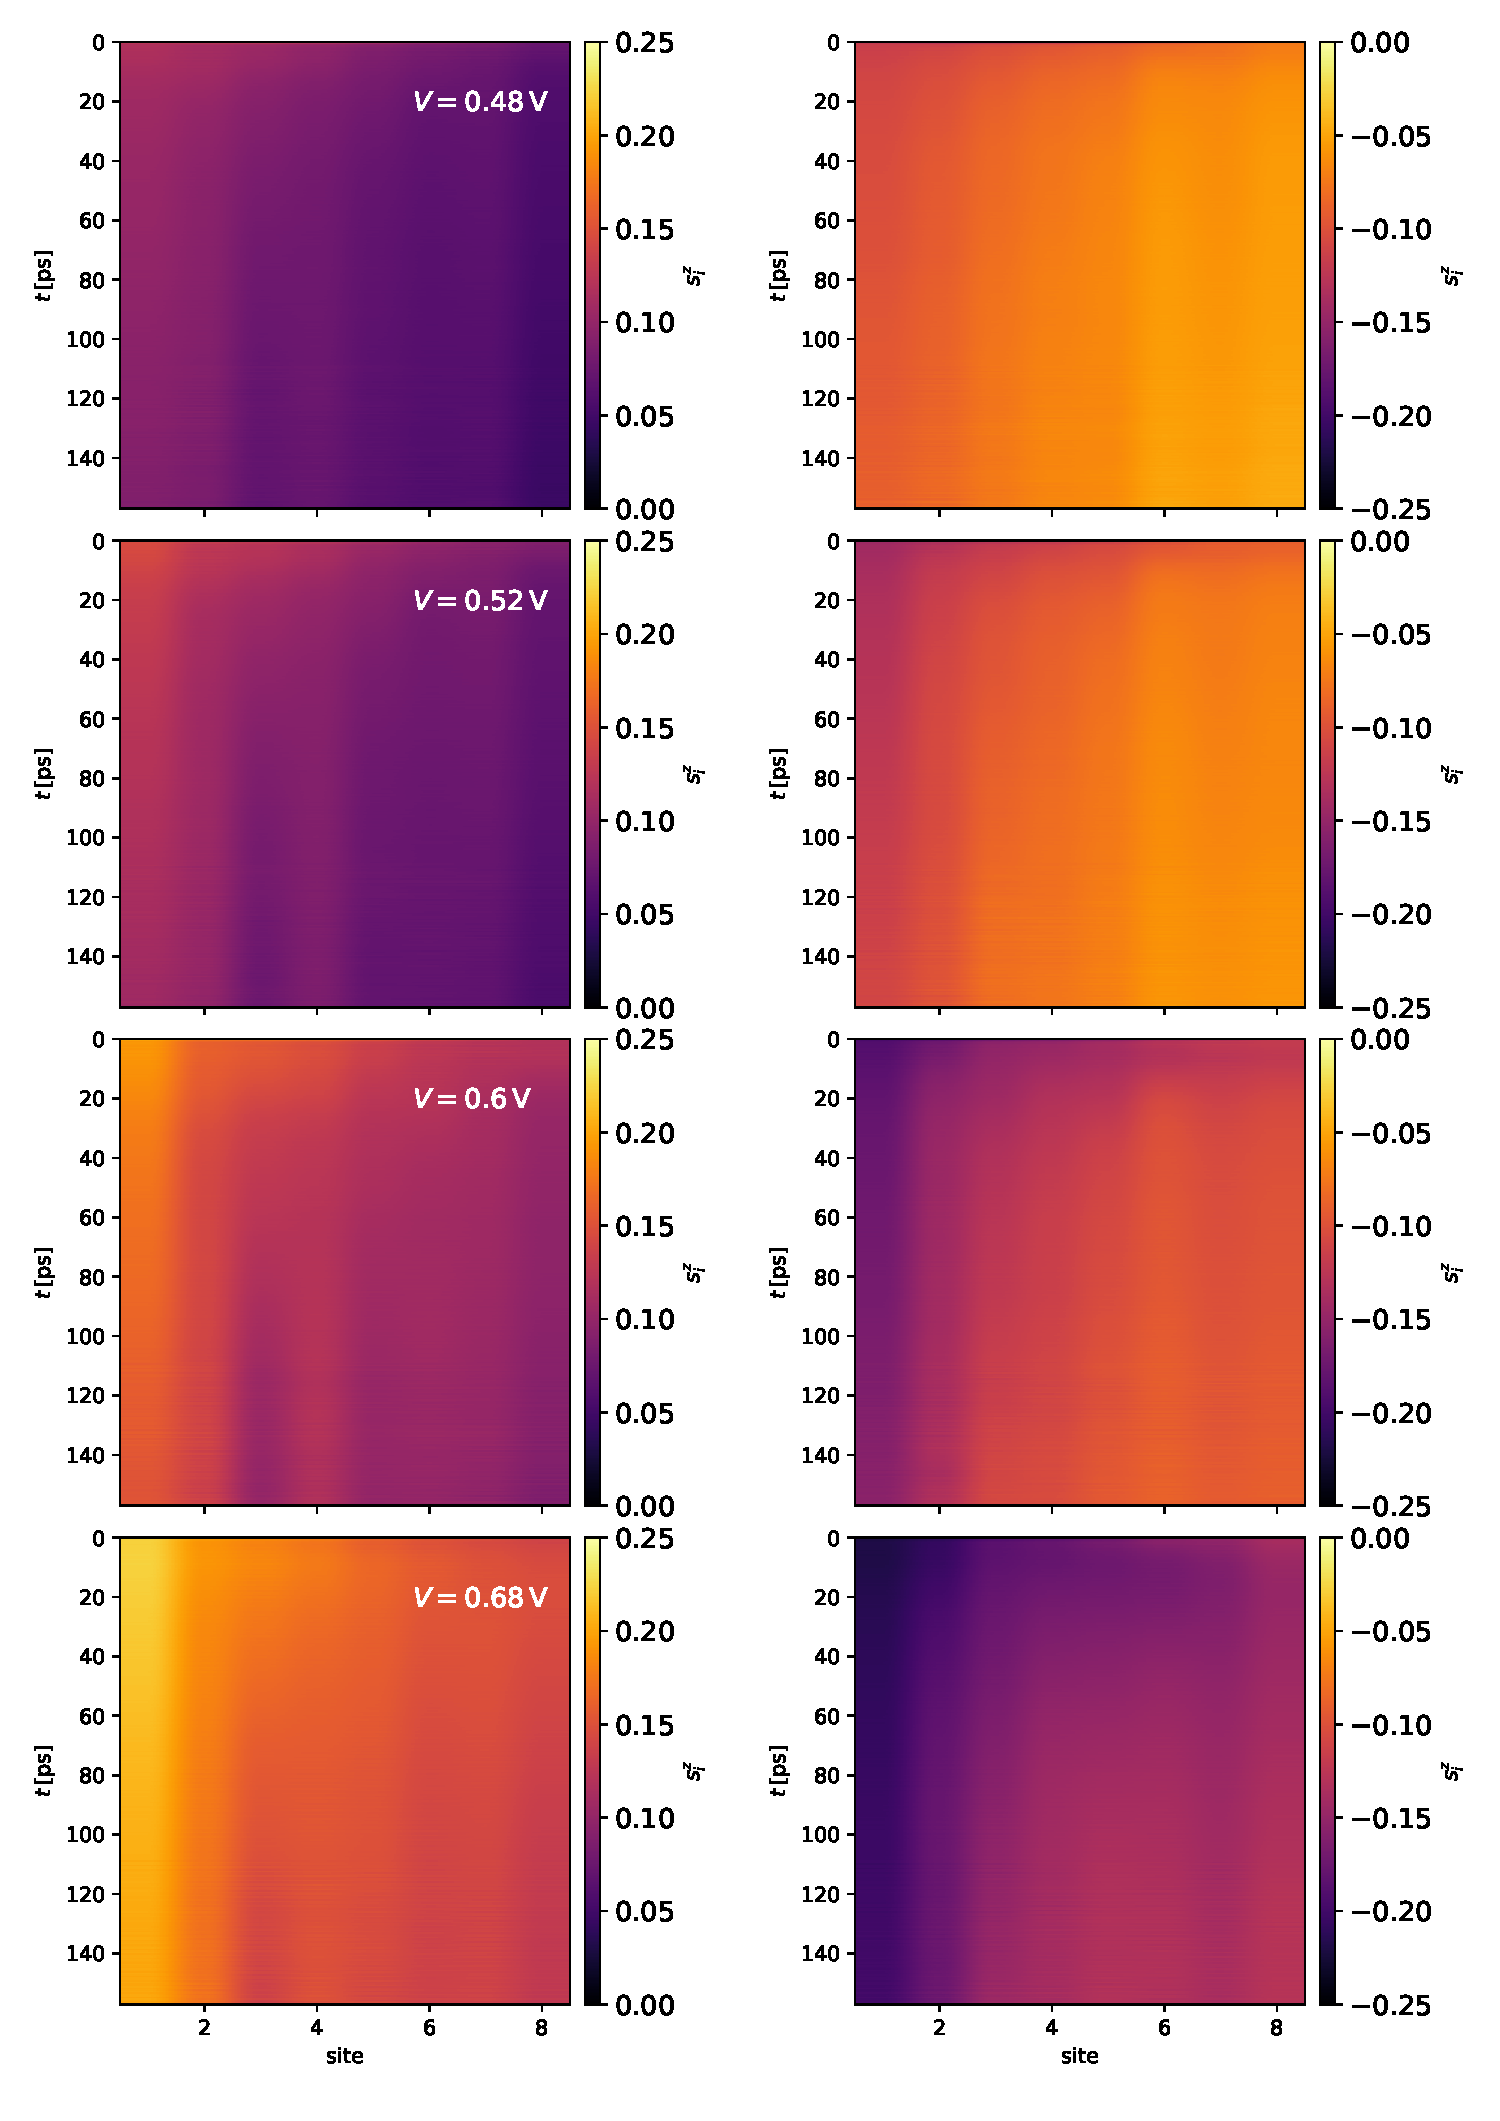
\includegraphics[width=0.9\textwidth]{figs/tsoPh10/L2x4_electrons_allV_tsoPh10.pdf}
	\caption{Space-time dependence of local spin polarization for various volage: Left $P=0.5$, Right column $P=-0.5$.}
\end{figure}
\begin{figure}[!h]
	\centering
	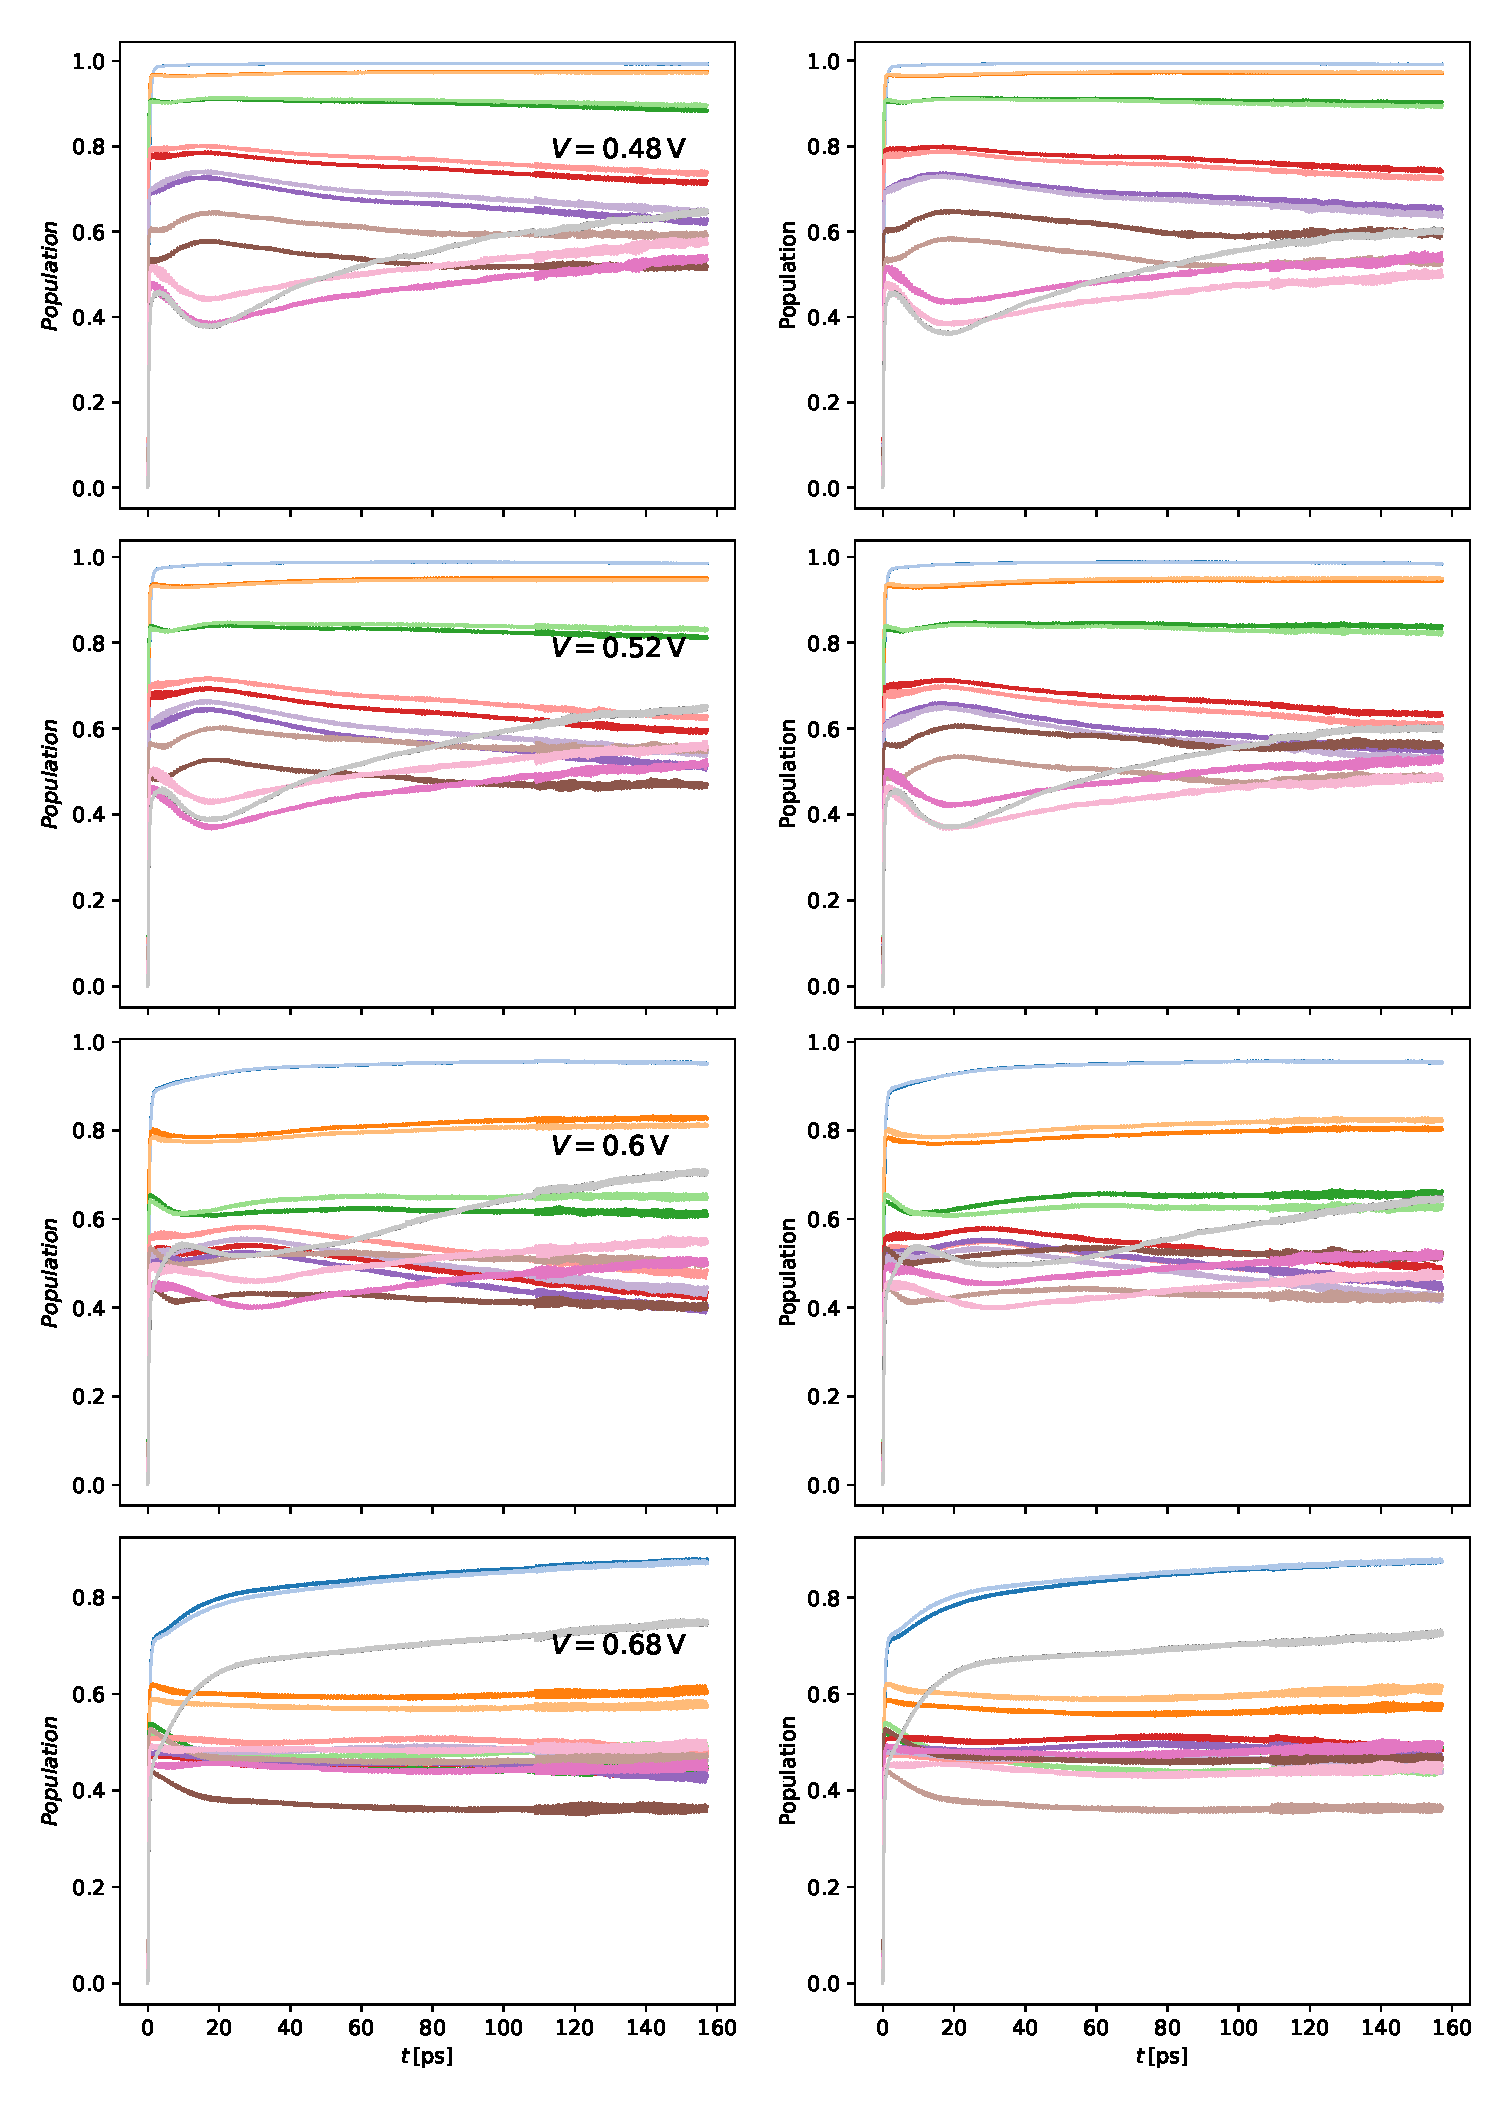
\includegraphics[width=0.9\textwidth]{figs/tsoPh10/L2x4_electrons_es_allV_tsoPh10.pdf}
	\caption{Population dynamics in the instantaneous eigenstate basis. Left $P=0.5$; Right column $P=-0.5$.}
\end{figure}
\begin{figure}[!h]
	\centering
	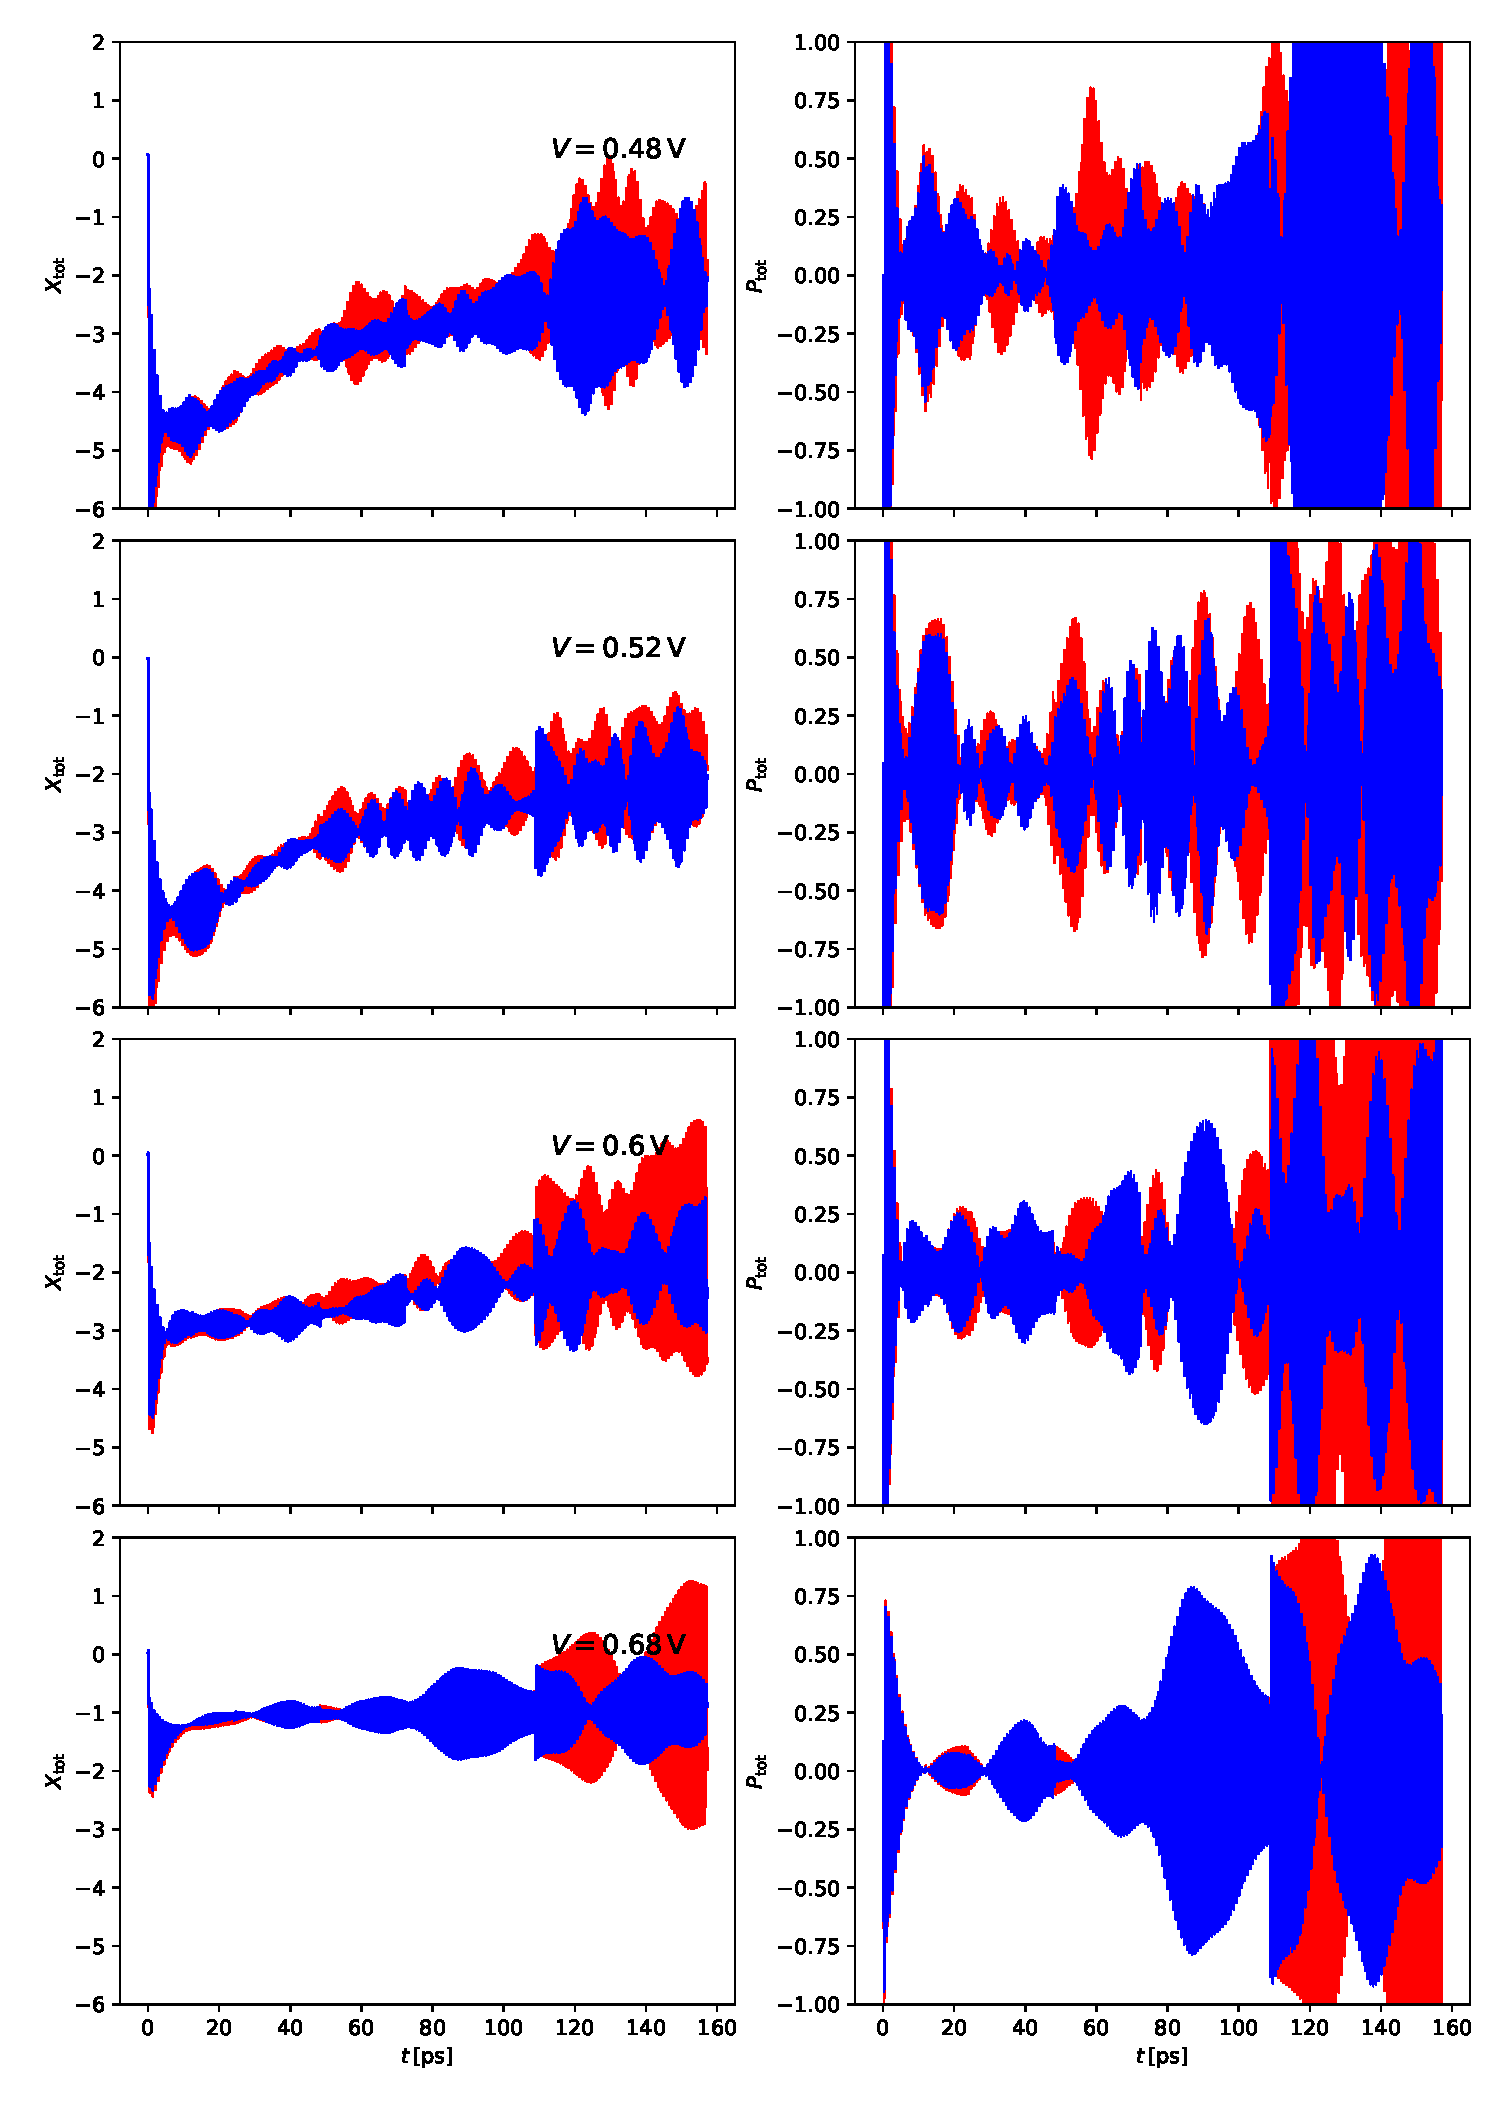
\includegraphics[width=0.9\textwidth]{figs/tsoPh10/L2x4_phonons_comb_allV_tsoPh10.pdf}
\end{figure}
\begin{figure}[!h]
	\centering
	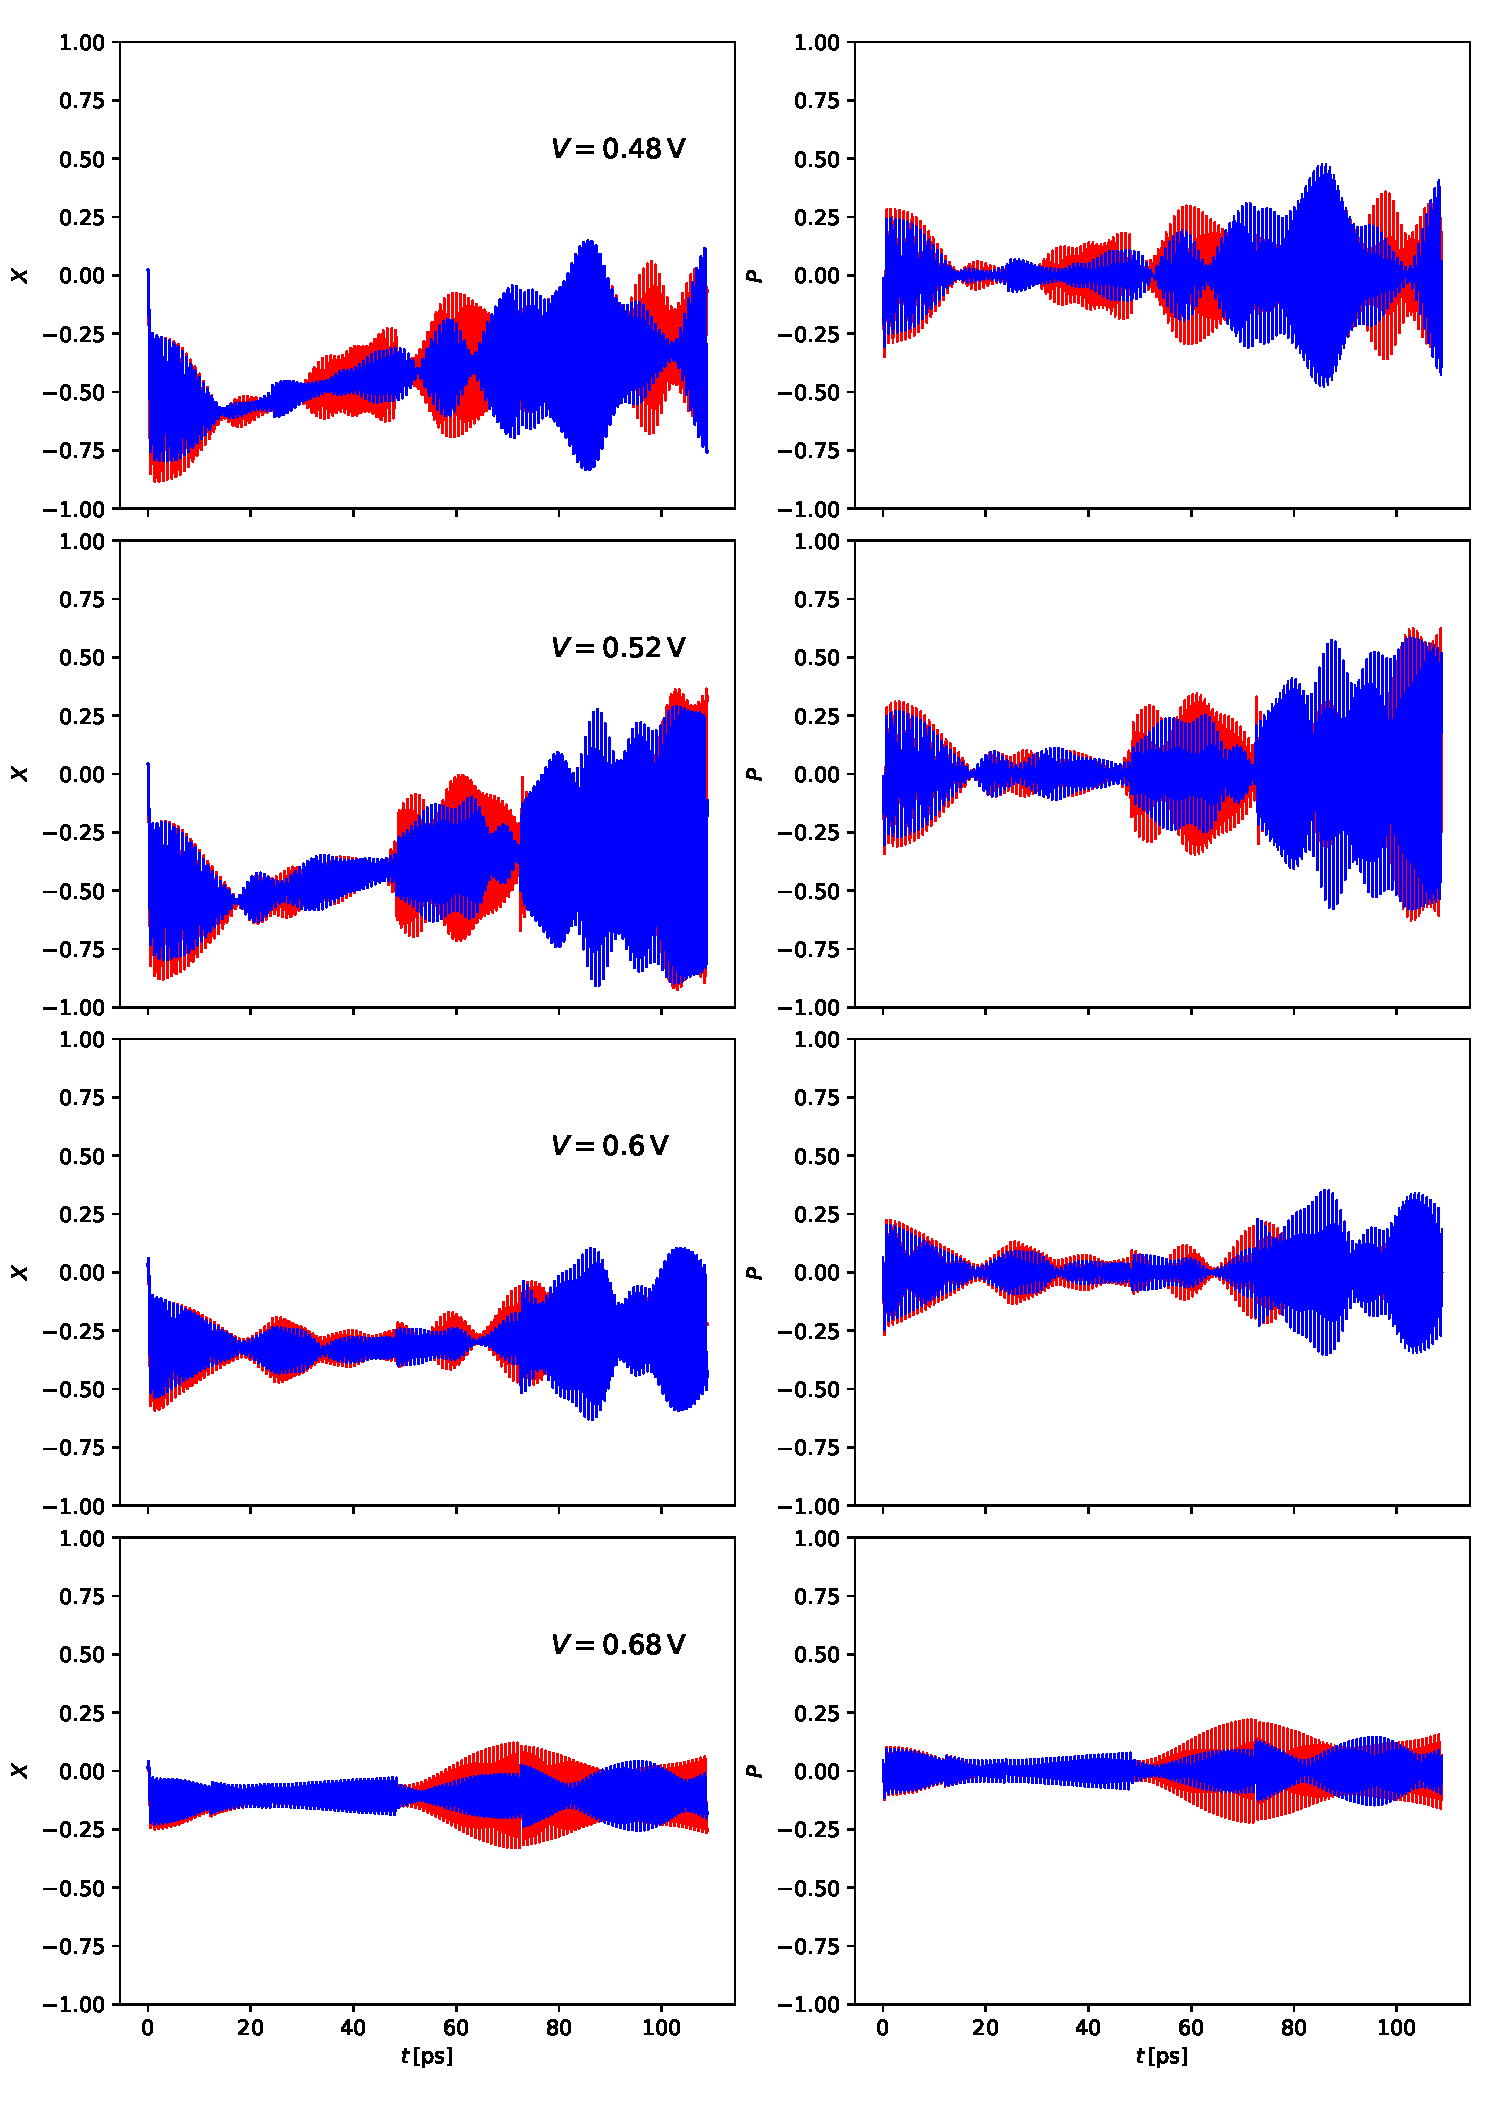
\includegraphics[width=0.9\textwidth]{figs/tsoPh10/L2x4_phonons_1_allV_tsoPh10.pdf}
	\caption{Phonon at bond 1 for $P=0.5$}
\end{figure}
\begin{figure}[!h]
	\centering
	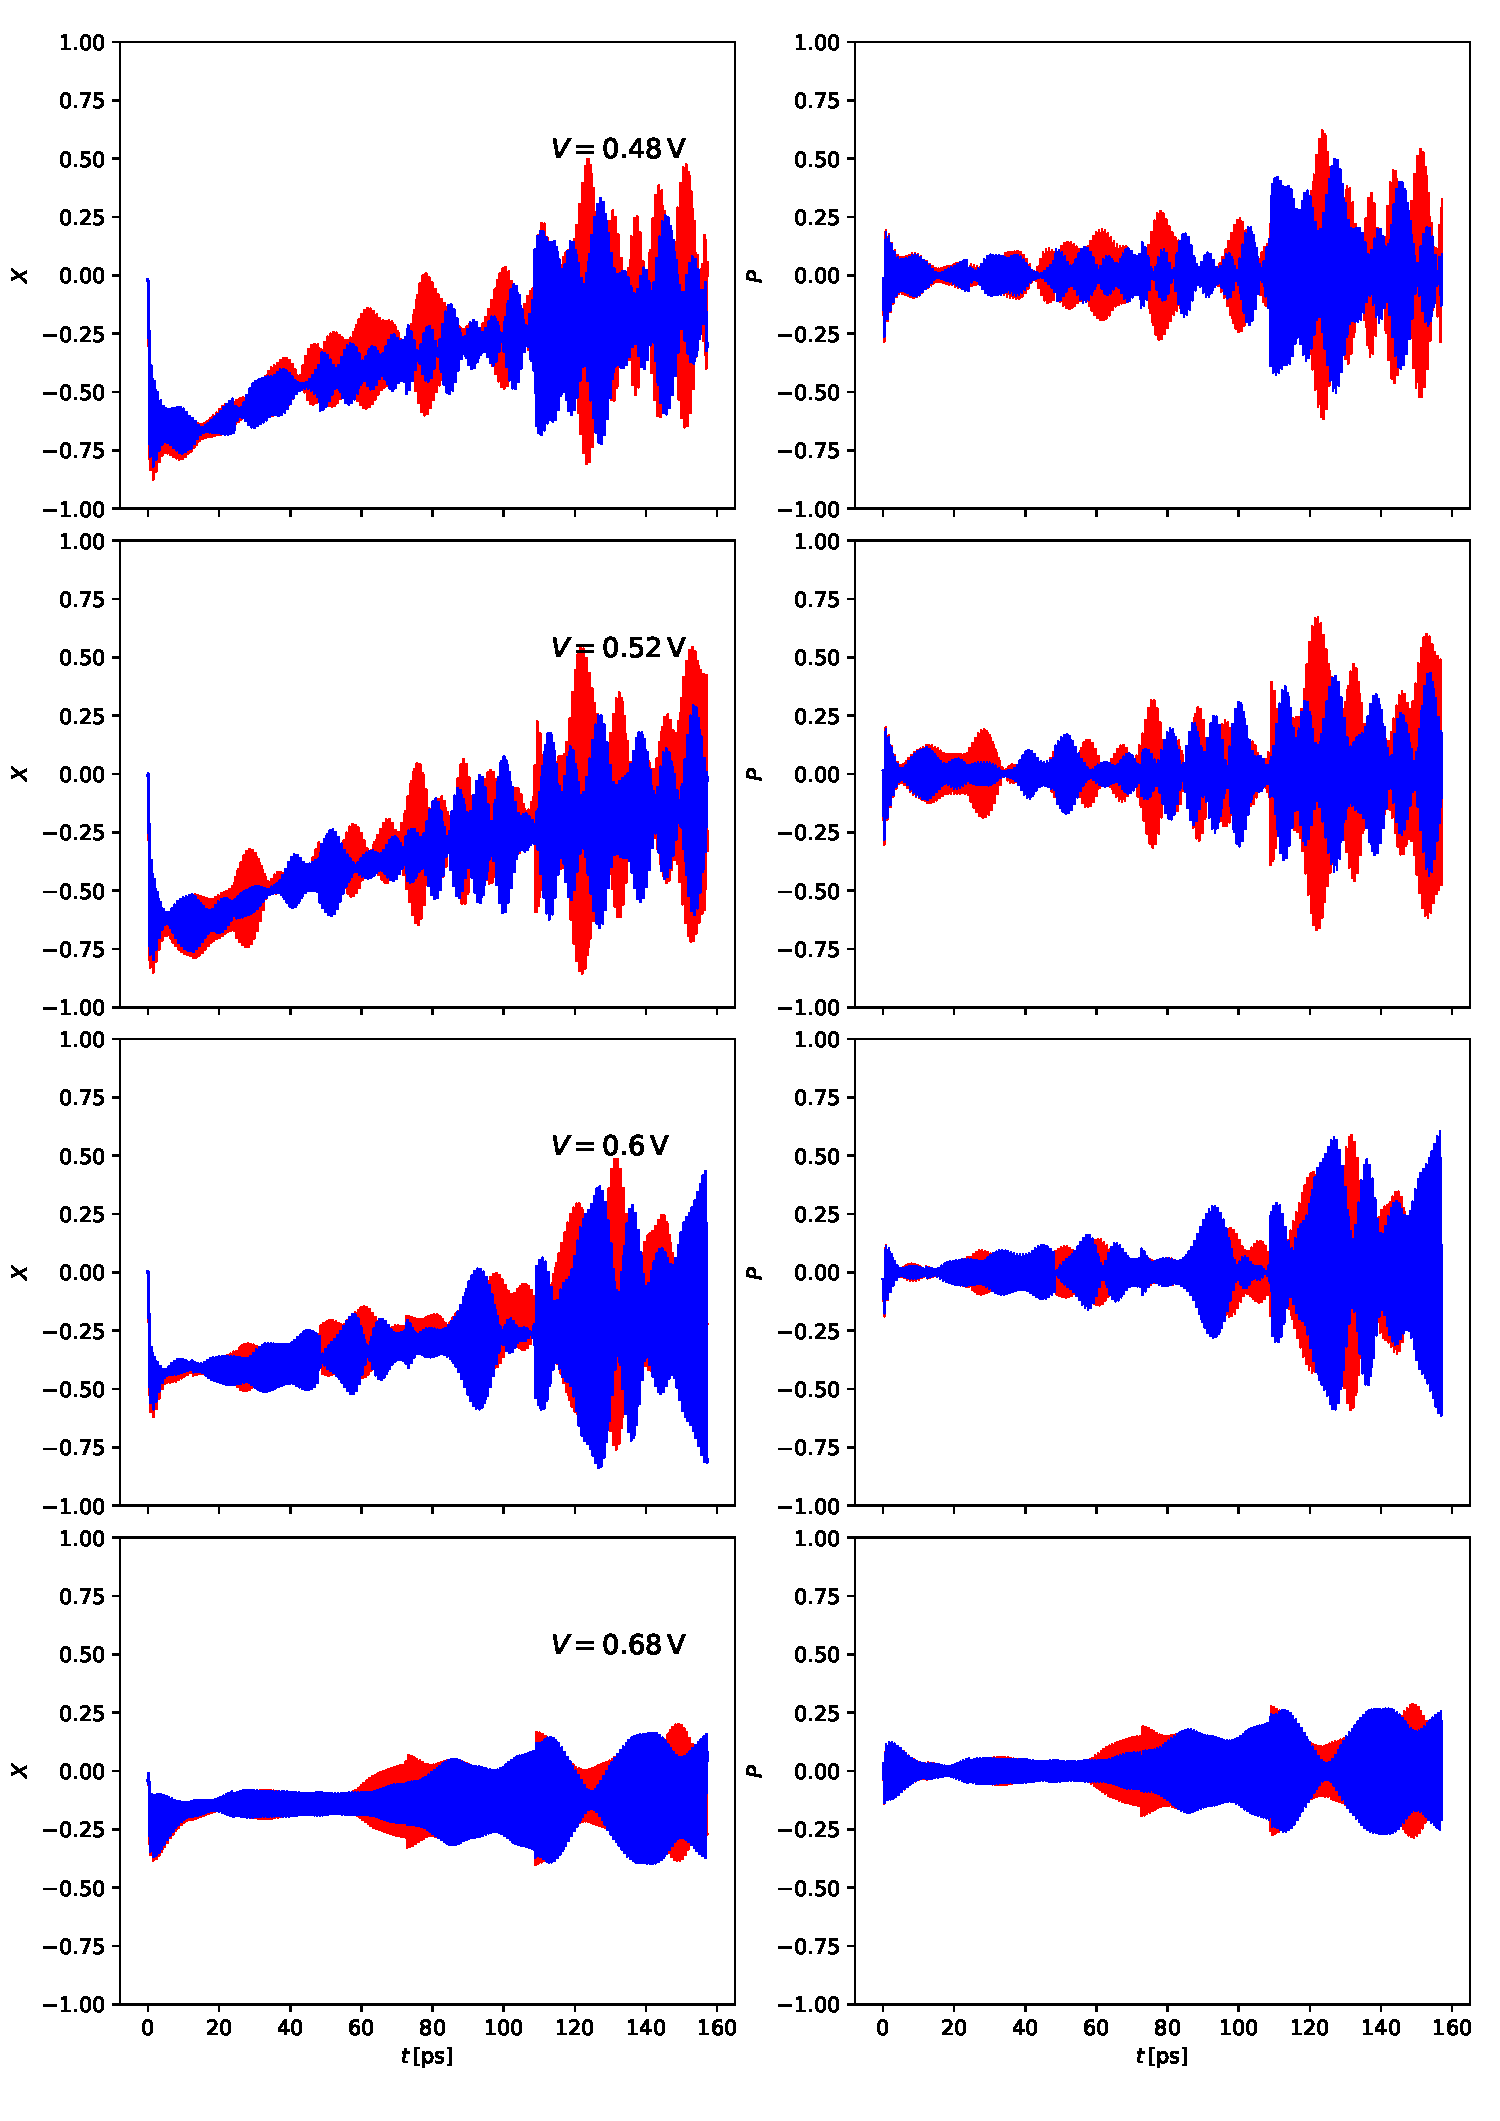
\includegraphics[width=0.9\textwidth]{figs/tsoPh10/L2x4_phonons_4_allV_tsoPh10.pdf}
	\caption{Phonon at bond 4 for $P=0.5$}
\end{figure}

\clearpage
\subsection{$L=2\times 4$, $\lambda_0=\SI{1}{\milli\electronvolt}$, $\lambda_1=\SI{10}{\milli\electronvolt}$, $\varepsilon_0=\SI{0}{\milli\electronvolt}$}
\begin{figure}[!h]
	\centering
	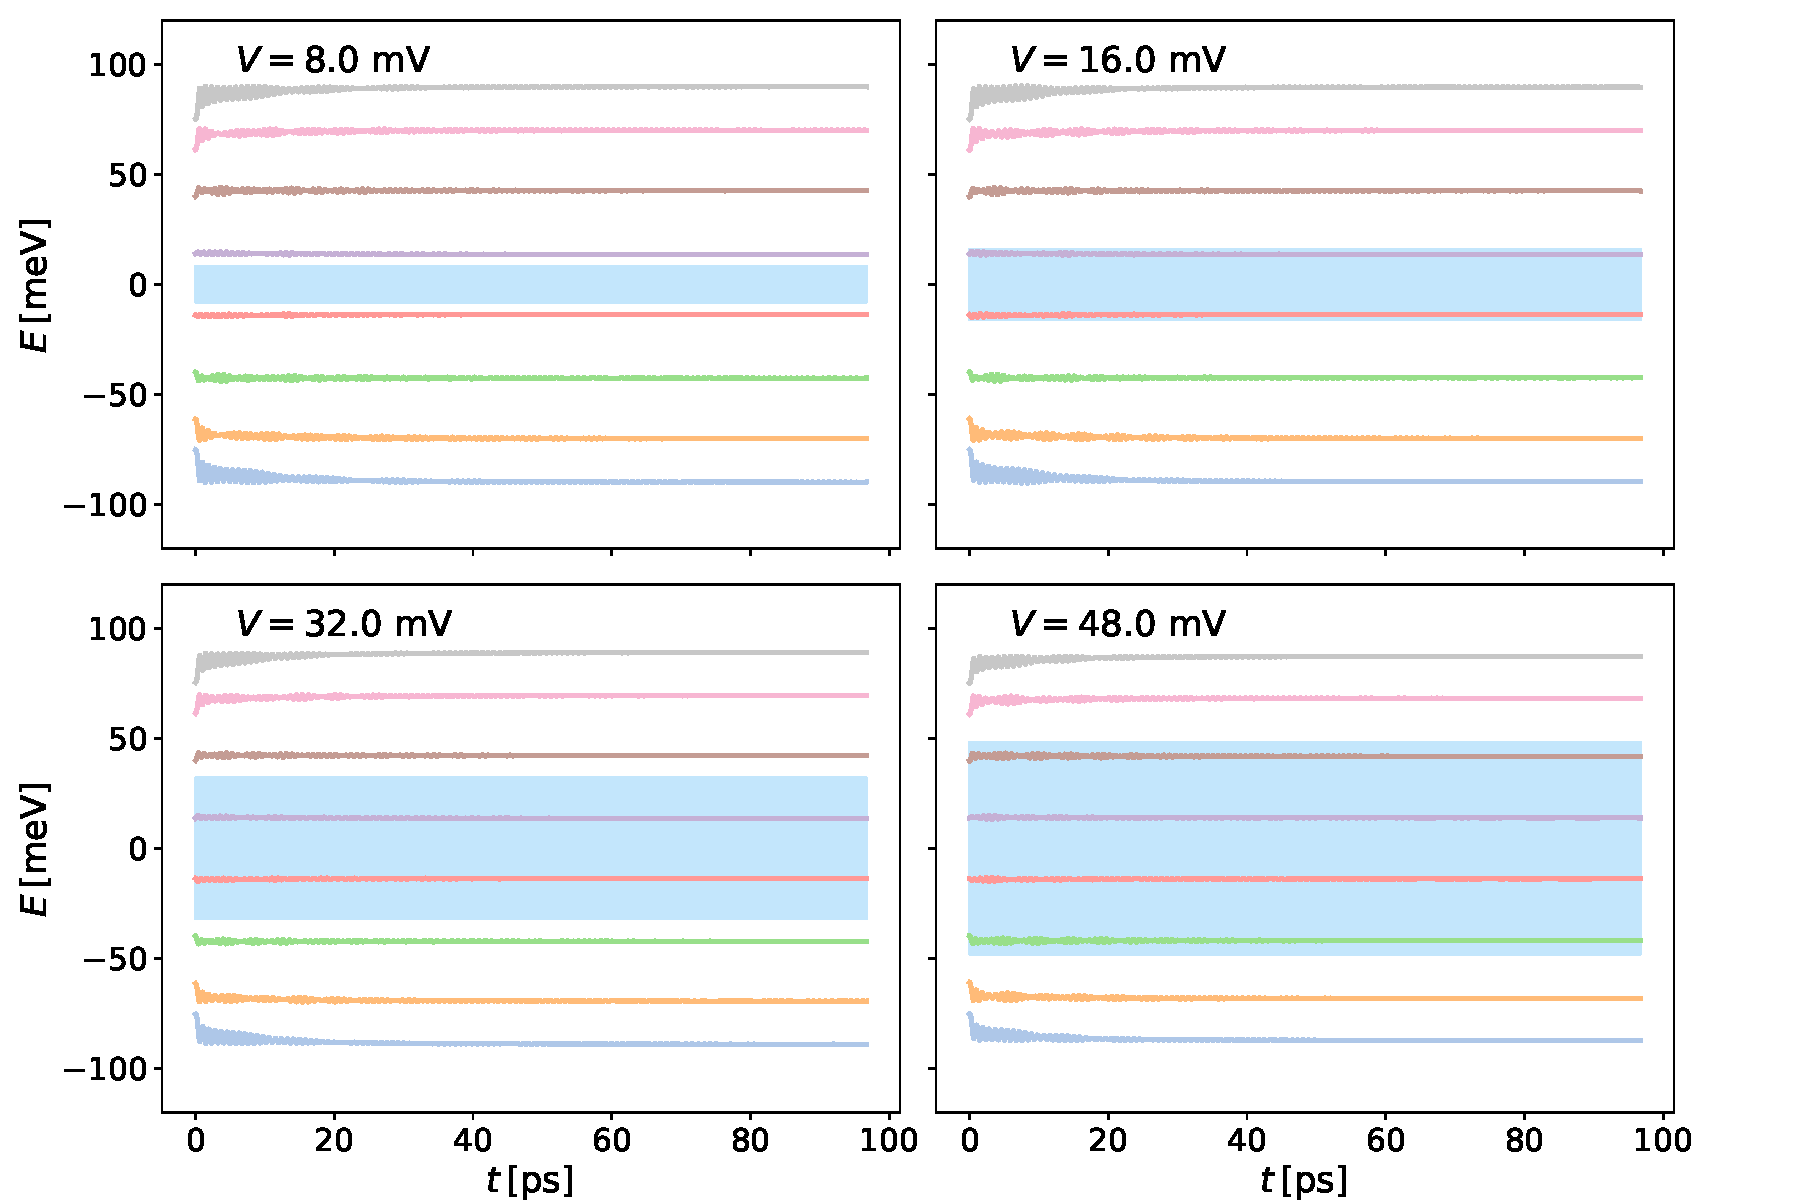
\includegraphics[width=0.9\textwidth]{figs/tsoPh10_eps0/L2x4_spectrumTD_PhAvg_tsoPh10.0_eps0.pdf}
	%~/PhD/projects/CISS_data/v2/I_V/w0_2_t1_4_tso_1_tsoPh_10_eps0/L2x4/v2
\end{figure}
\begin{figure}[!h]
	\centering
	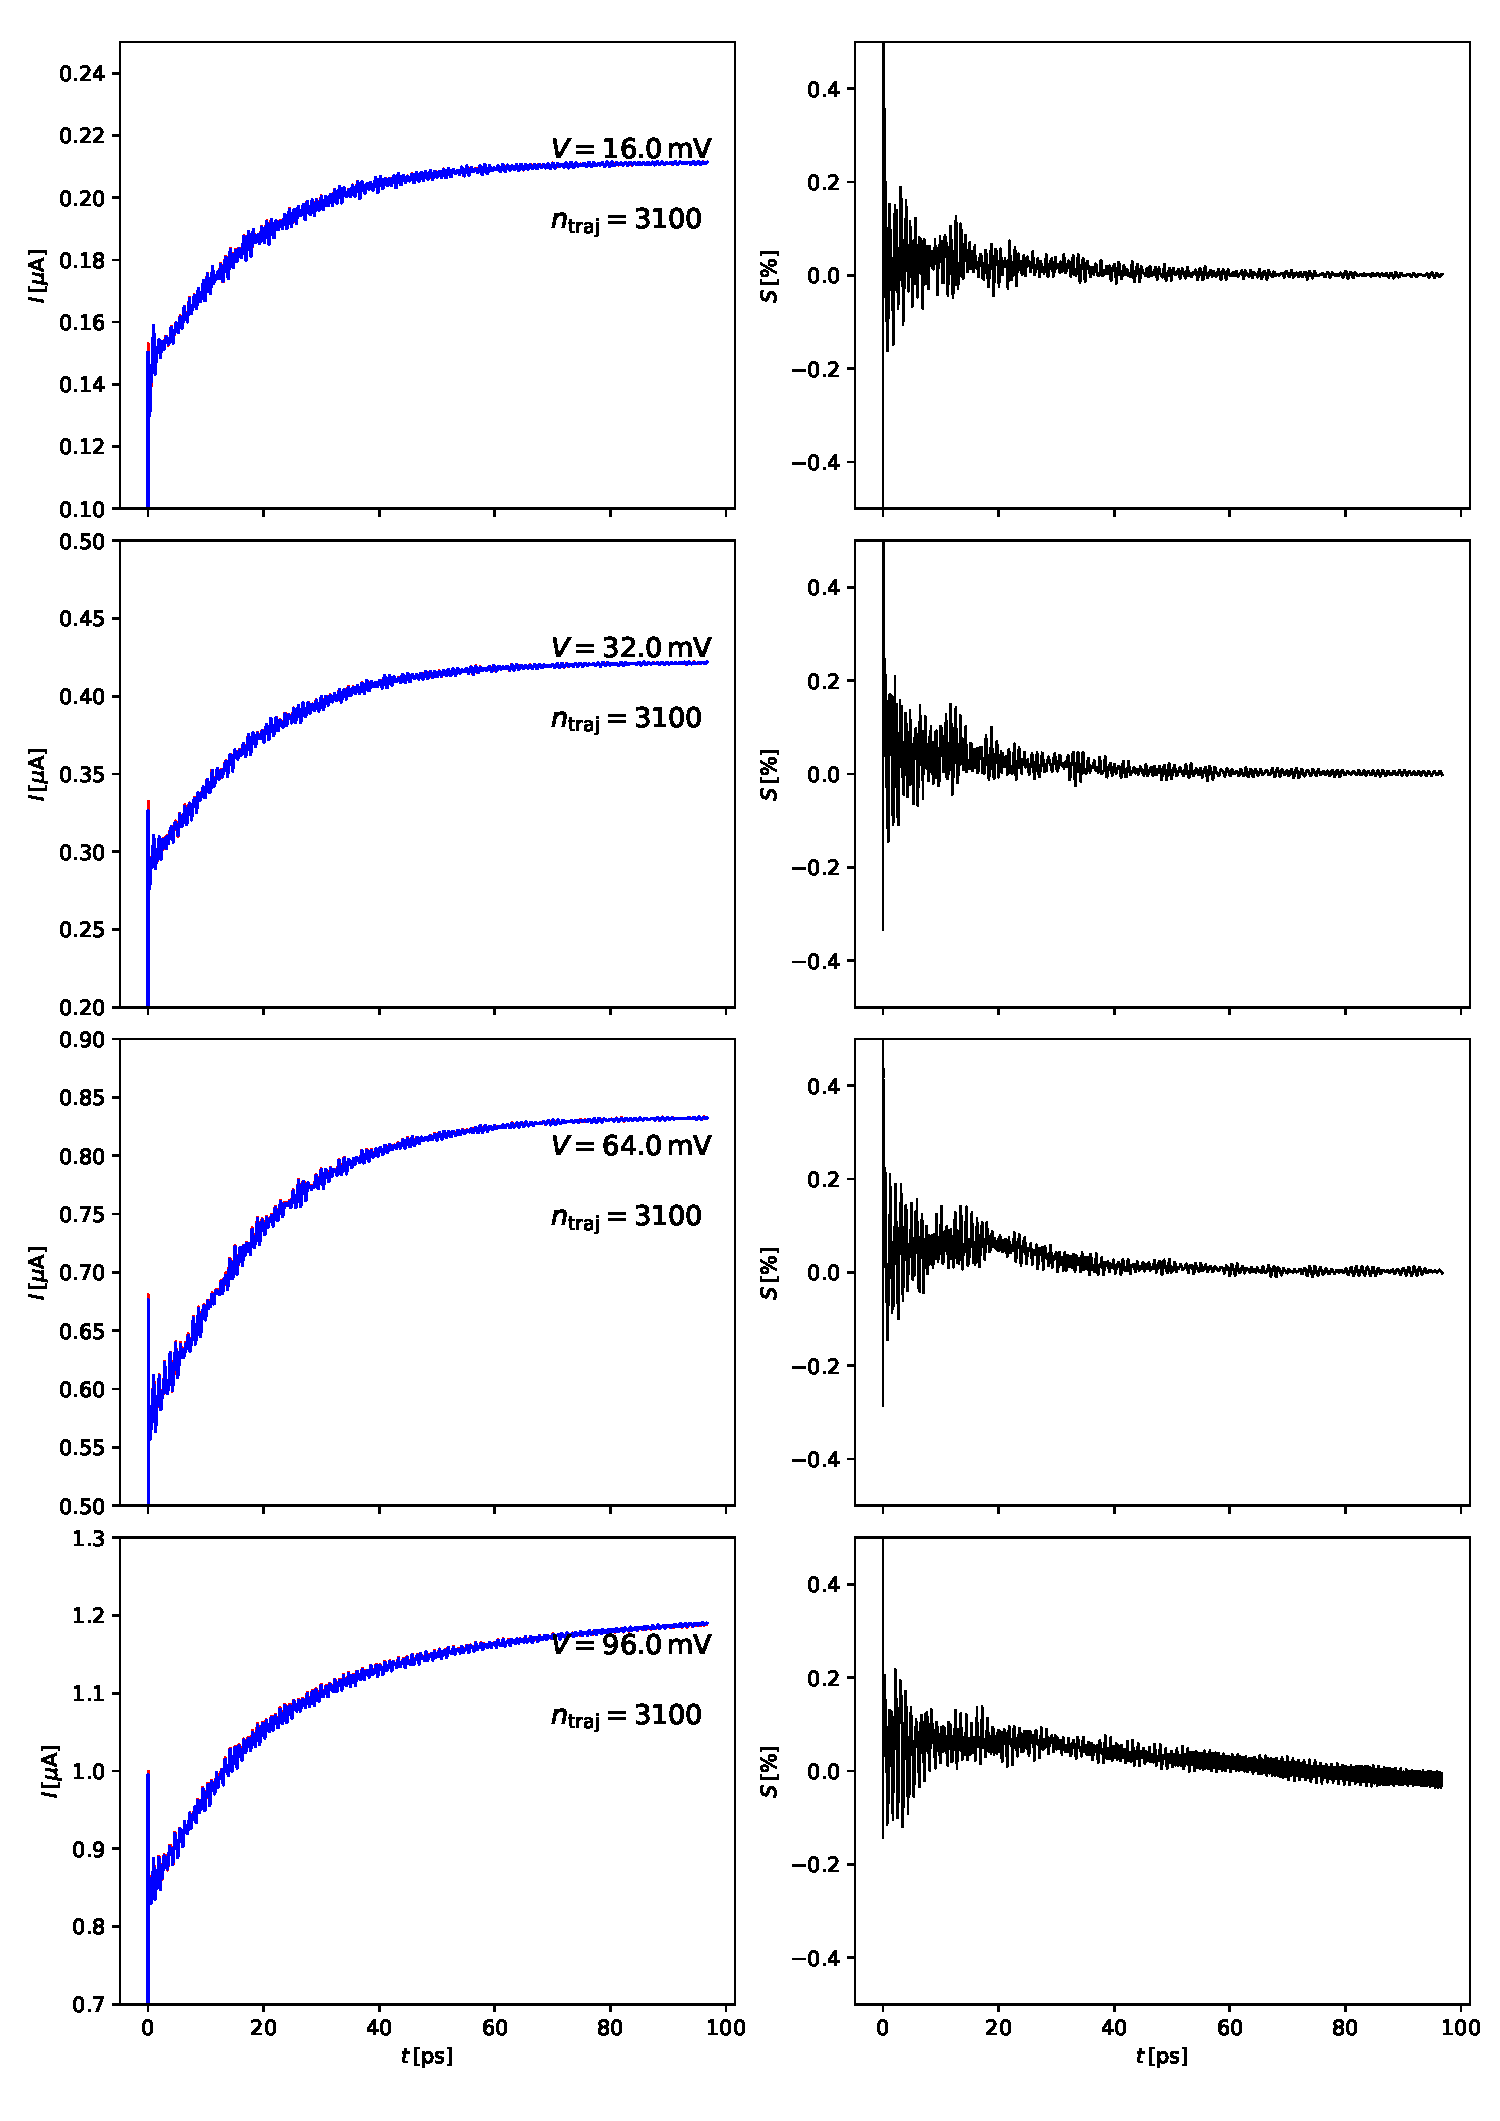
\includegraphics[width=0.9\textwidth]{figs/tsoPh10_eps0/L2x4_currents_MR_allV_tsoPh10_eps0.pdf}
	%~/PhD/projects/CISS_data/v2/I_V/w0_2_t1_4_tso_1_tsoPh_10_eps0/L2x4/v2
\end{figure}
\begin{figure}[!h]
	\centering
	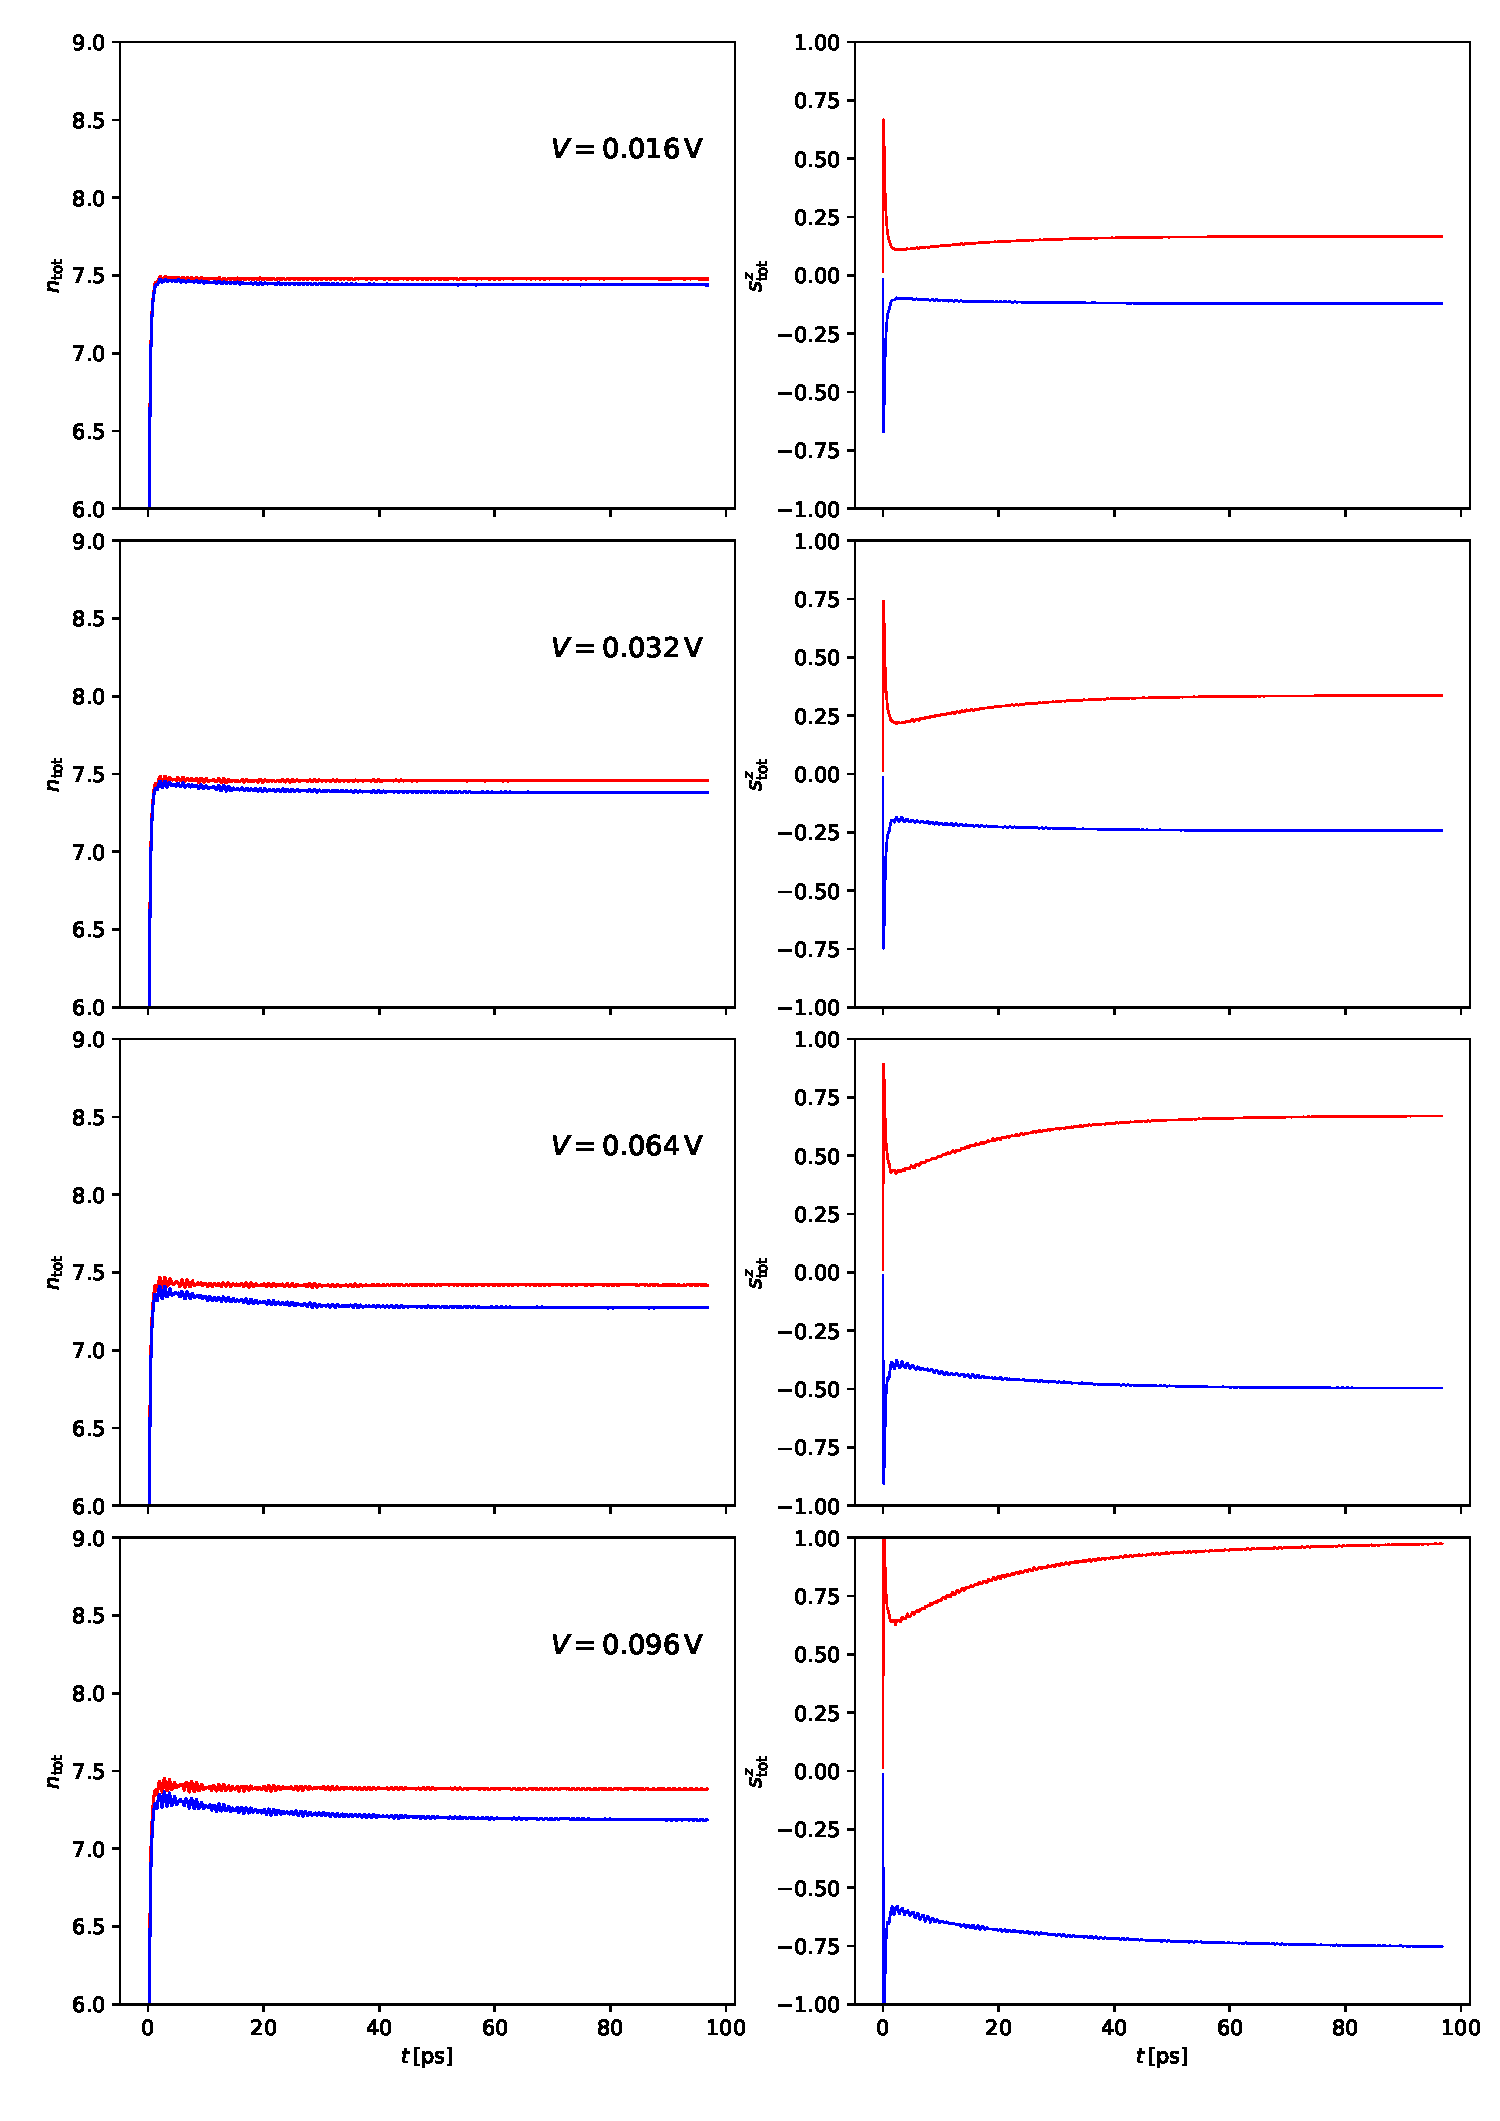
\includegraphics[width=0.9\textwidth]{figs/tsoPh10_eps0/L2x4_charge_sz_tot_allV_tsoPh10_eps0.pdf}
	%~/PhD/projects/CISS_data/v2/I_V/w0_2_t1_4_tso_1_tsoPh_10_eps0/L2x4/v2
\end{figure}

\begin{figure}[!h]
	\centering
	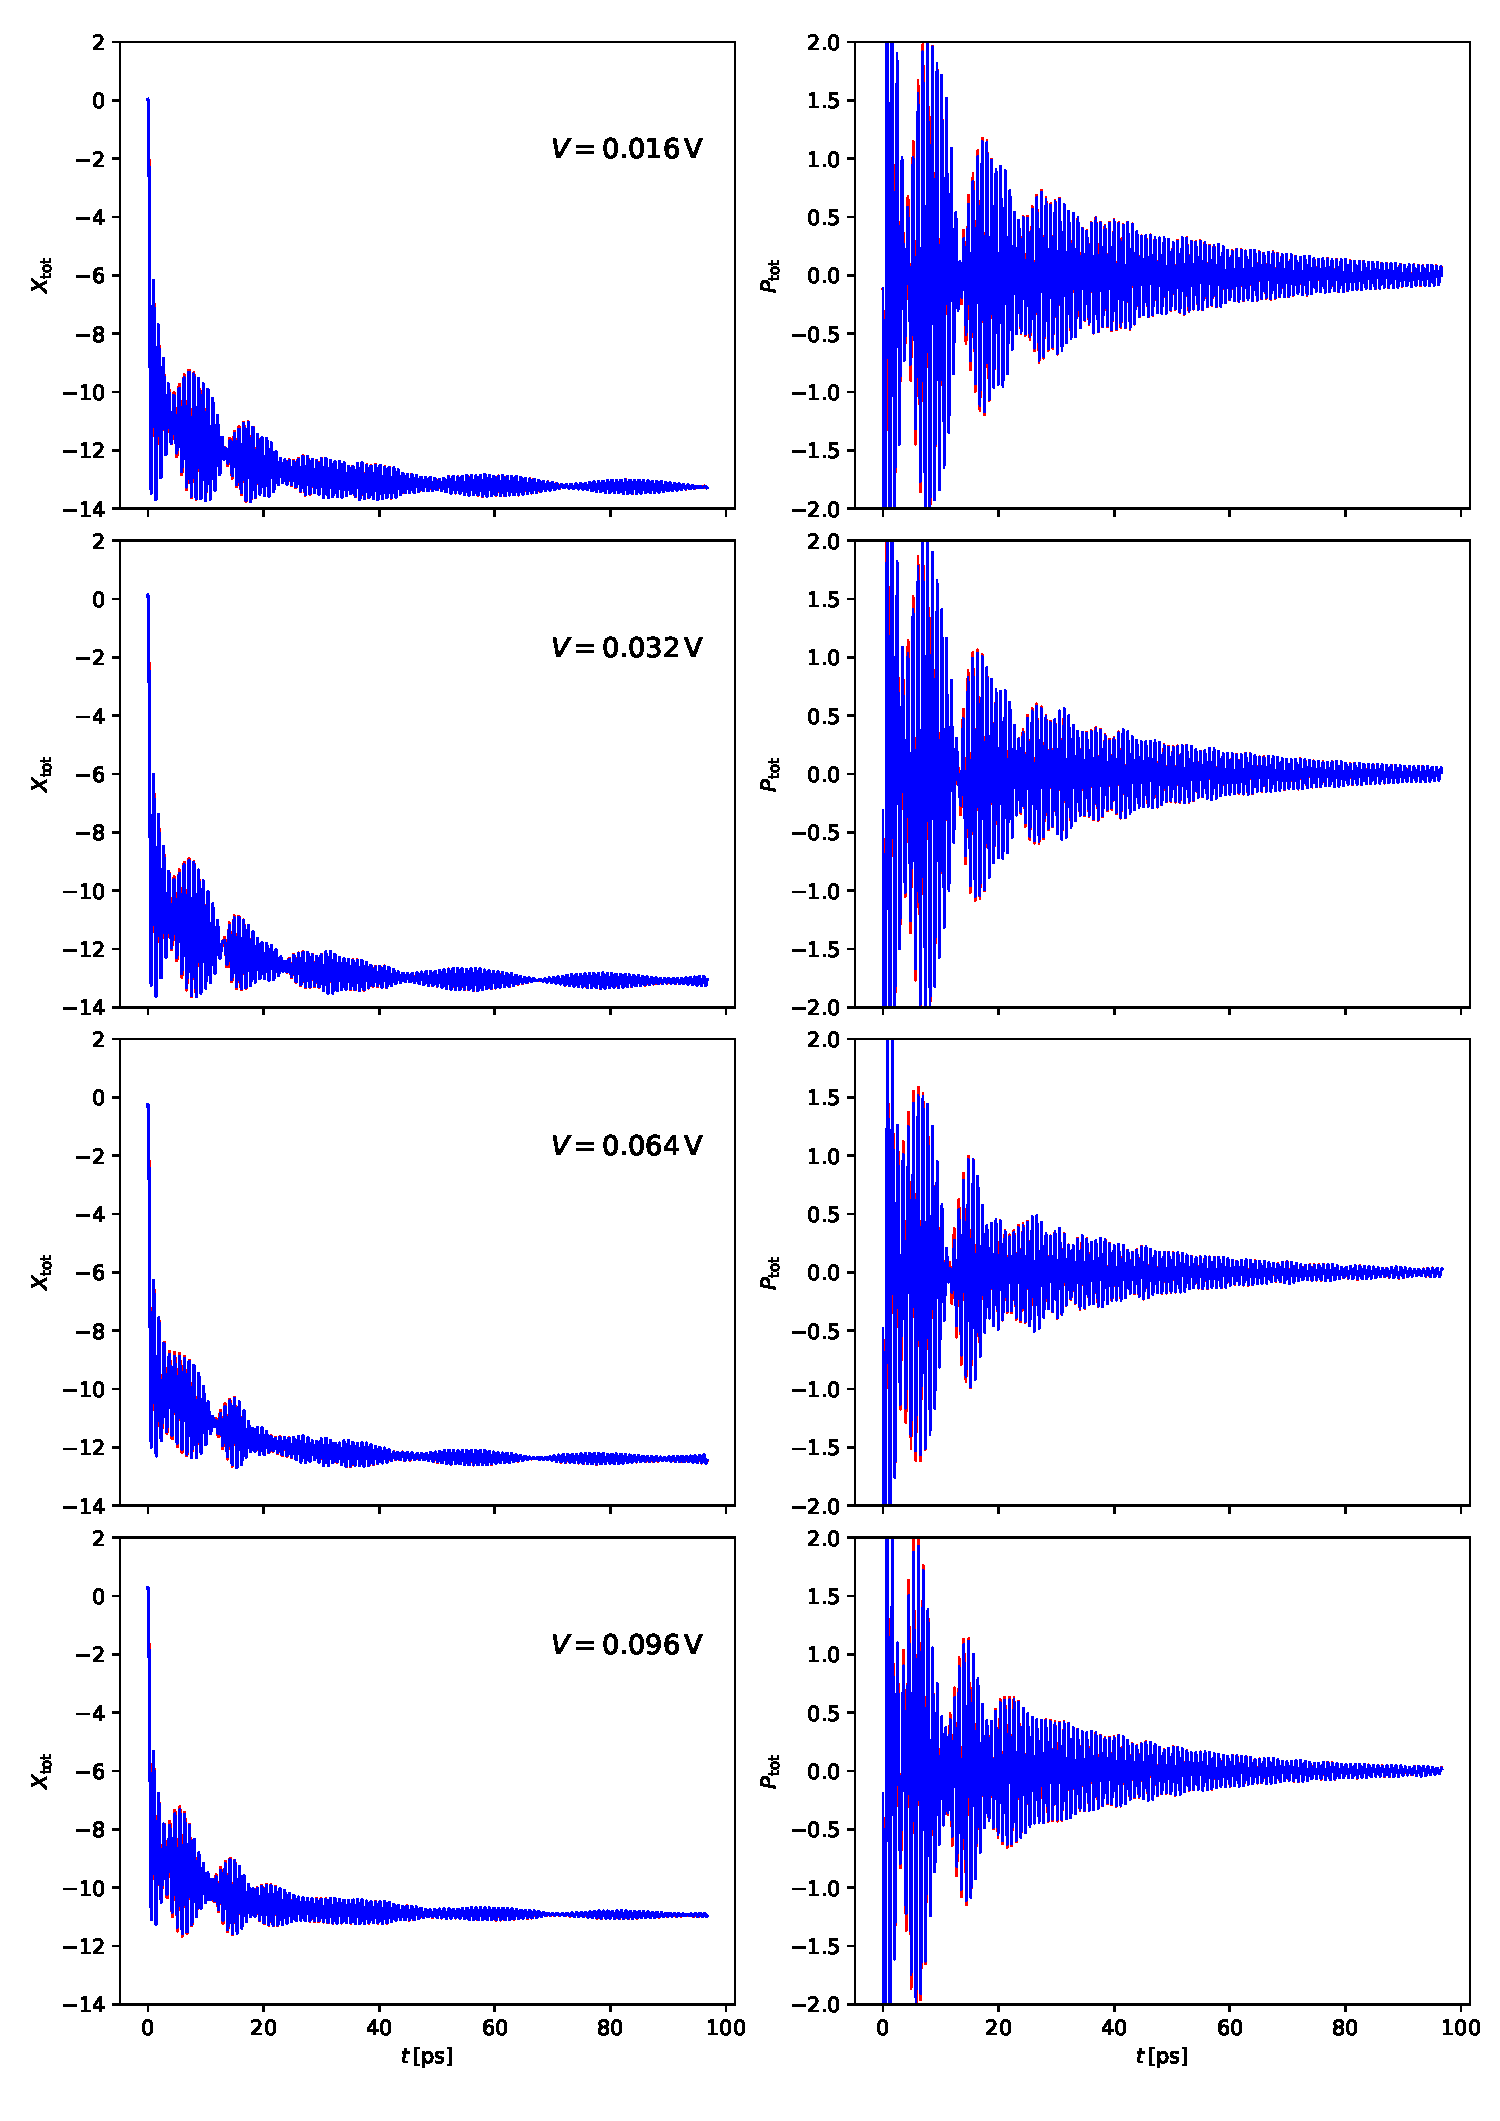
\includegraphics[width=0.9\textwidth]{figs/tsoPh10_eps0/L2x4_phonons_comb_allV_tsoPh10_eps0.pdf}
	%~/PhD/projects/CISS_data/v2/I_V/w0_2_t1_4_tso_1_tsoPh_10_eps0/L2x4/v2
\end{figure}
\clearpage
\subsubsection{Combined picture: Current, electron and vibrational dynamics}
\begin{figure}[!h]
	\centering
	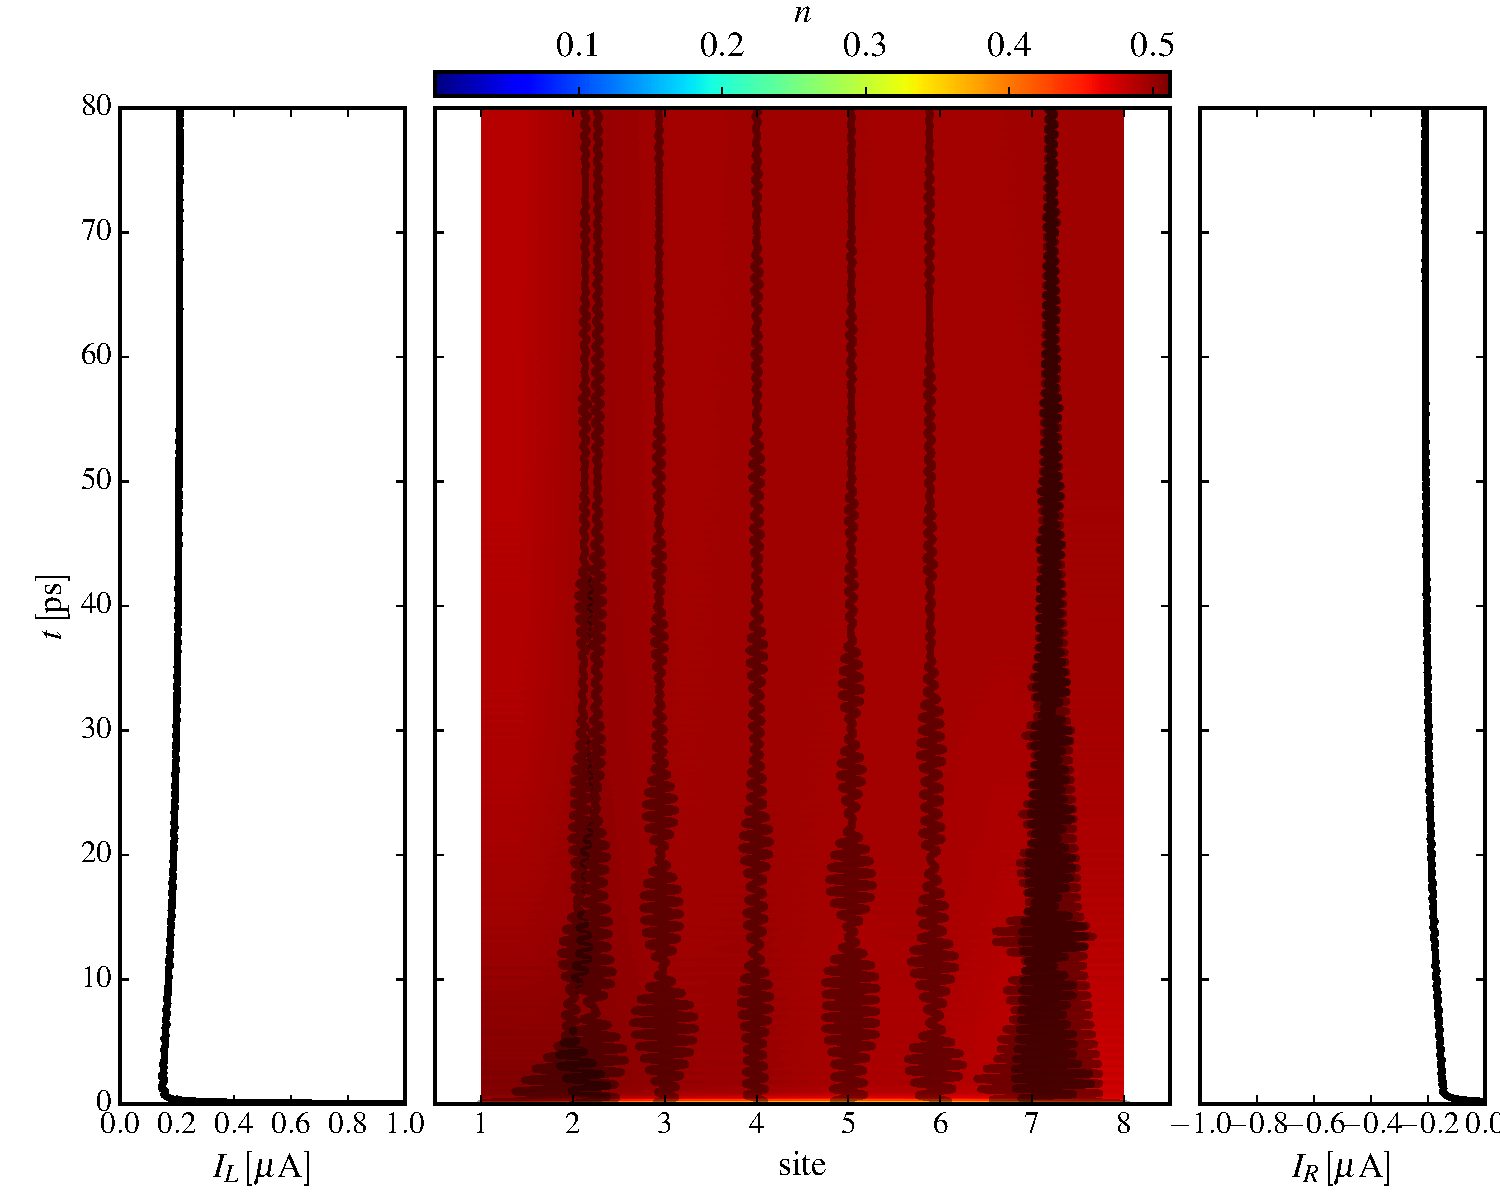
\includegraphics[width=0.8\textwidth]{figs/tsoPh10_eps0/L8_V4_tPh0.004_tso0.001_tsoPh0.01_eps0_P_electrons_tend80_currents_phonons.pdf}\\
	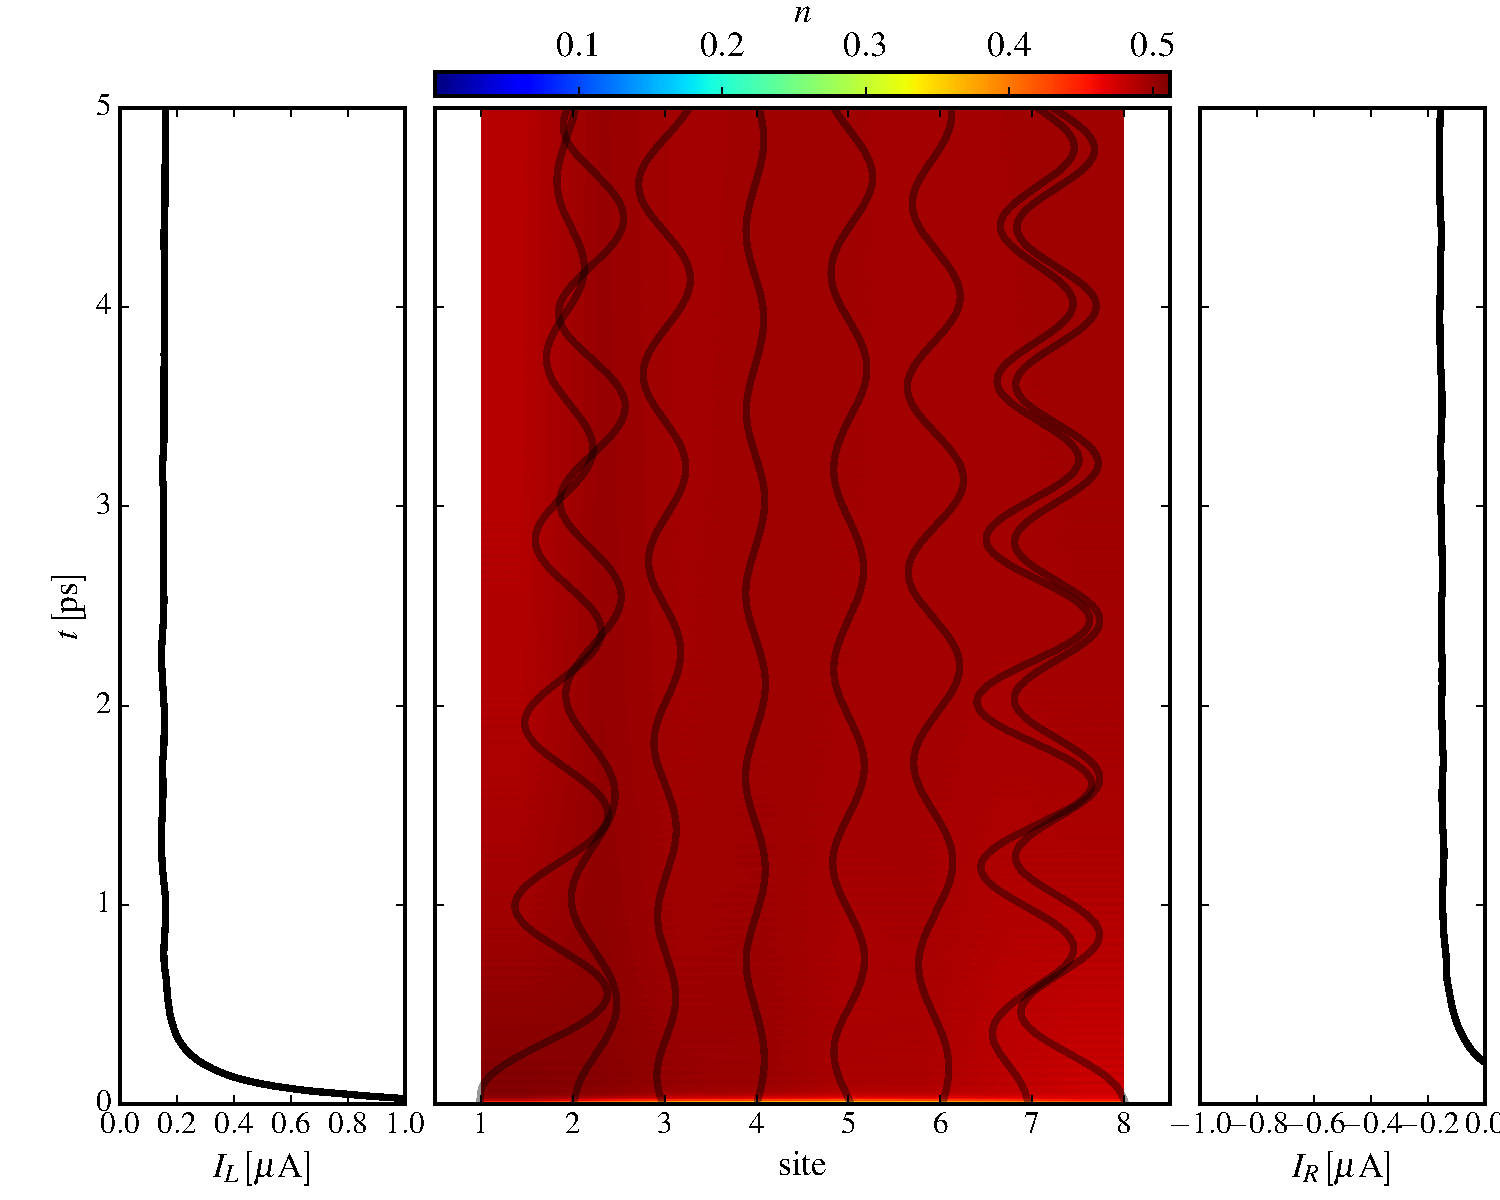
\includegraphics[width=0.8\textwidth]{figs/tsoPh10_eps0/L8_V4_tPh0.004_tso0.001_tsoPh0.01_eps0_P_electrons_tend5_currents_phonons.pdf}
	\caption{For $V=\SI{16}{\milli\volt}$ and $P=0.5$.}
	%~/PhD/projects/CISS_data/v2/I_V/w0_2_t1_4_tso_1_tsoPh_10_eps0/L2x4/comb
\end{figure}
\begin{figure}[!h]
	\centering
	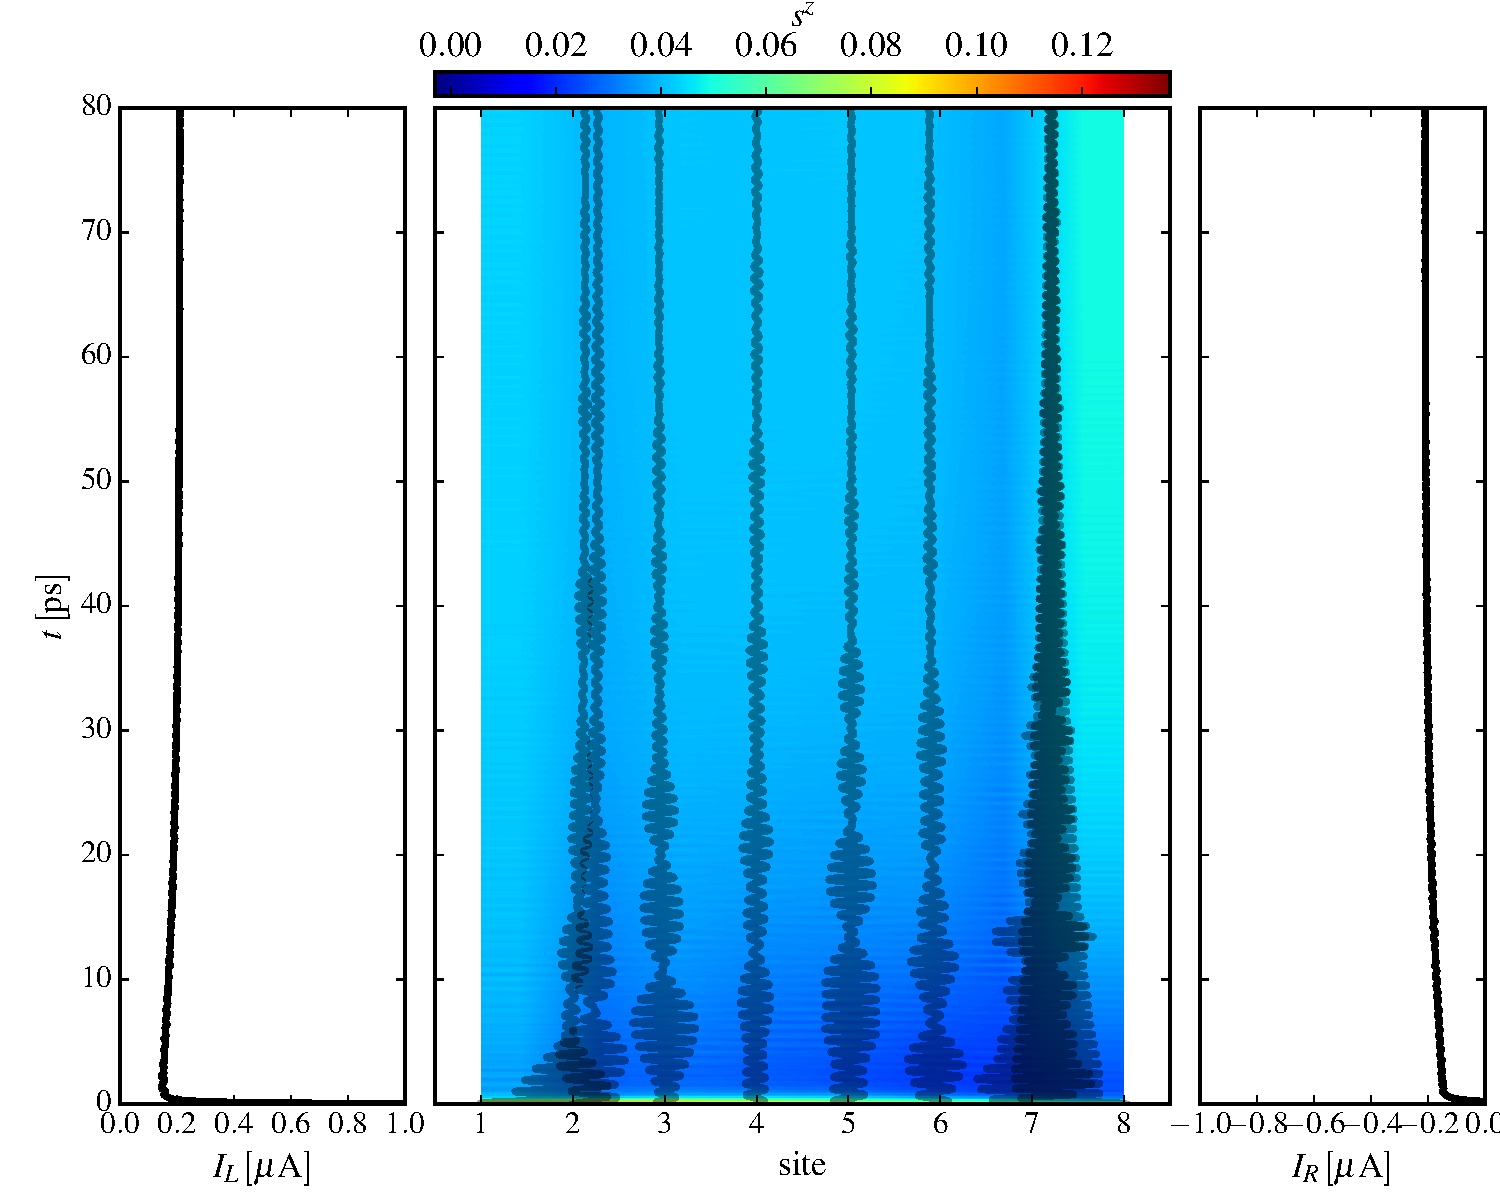
\includegraphics[width=0.8\textwidth]{figs/tsoPh10_eps0/L8_V4_tPh0.004_tso0.001_tsoPh0.01_eps0_P_spin_tend80_currents_phonons.pdf}\\
	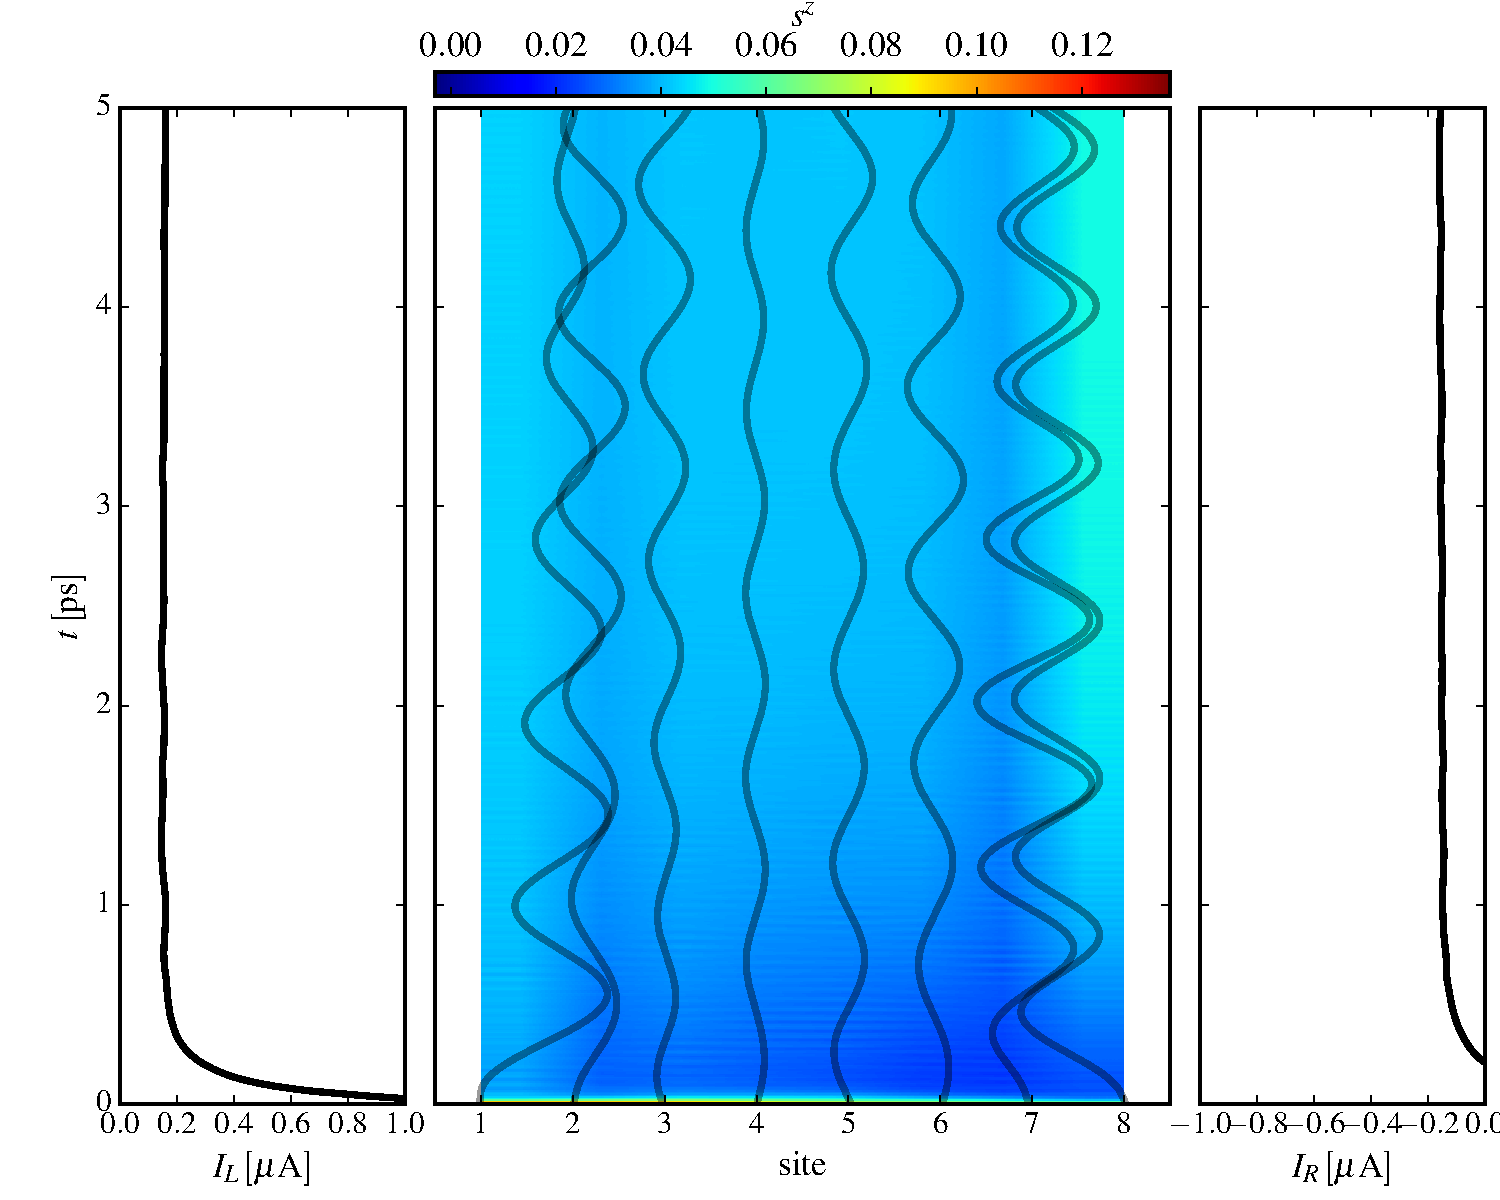
\includegraphics[width=0.8\textwidth]{figs/tsoPh10_eps0/L8_V4_tPh0.004_tso0.001_tsoPh0.01_eps0_P_spin_tend5_currents_phonons.pdf}
	\caption{For $V=\SI{16}{\milli\volt}$ and $P=0.5$.}
	%~/PhD/projects/CISS_data/v2/I_V/w0_2_t1_4_tso_1_tsoPh_10_eps0/L2x4/comb
\end{figure}


\clearpage
\subsection{$L=3\times 4$, $\lambda_0=\SI{1}{\milli\electronvolt}$, $\lambda_1=\SI{0.1}{\milli\electronvolt}$}
\begin{figure}[!h]
	\centering
	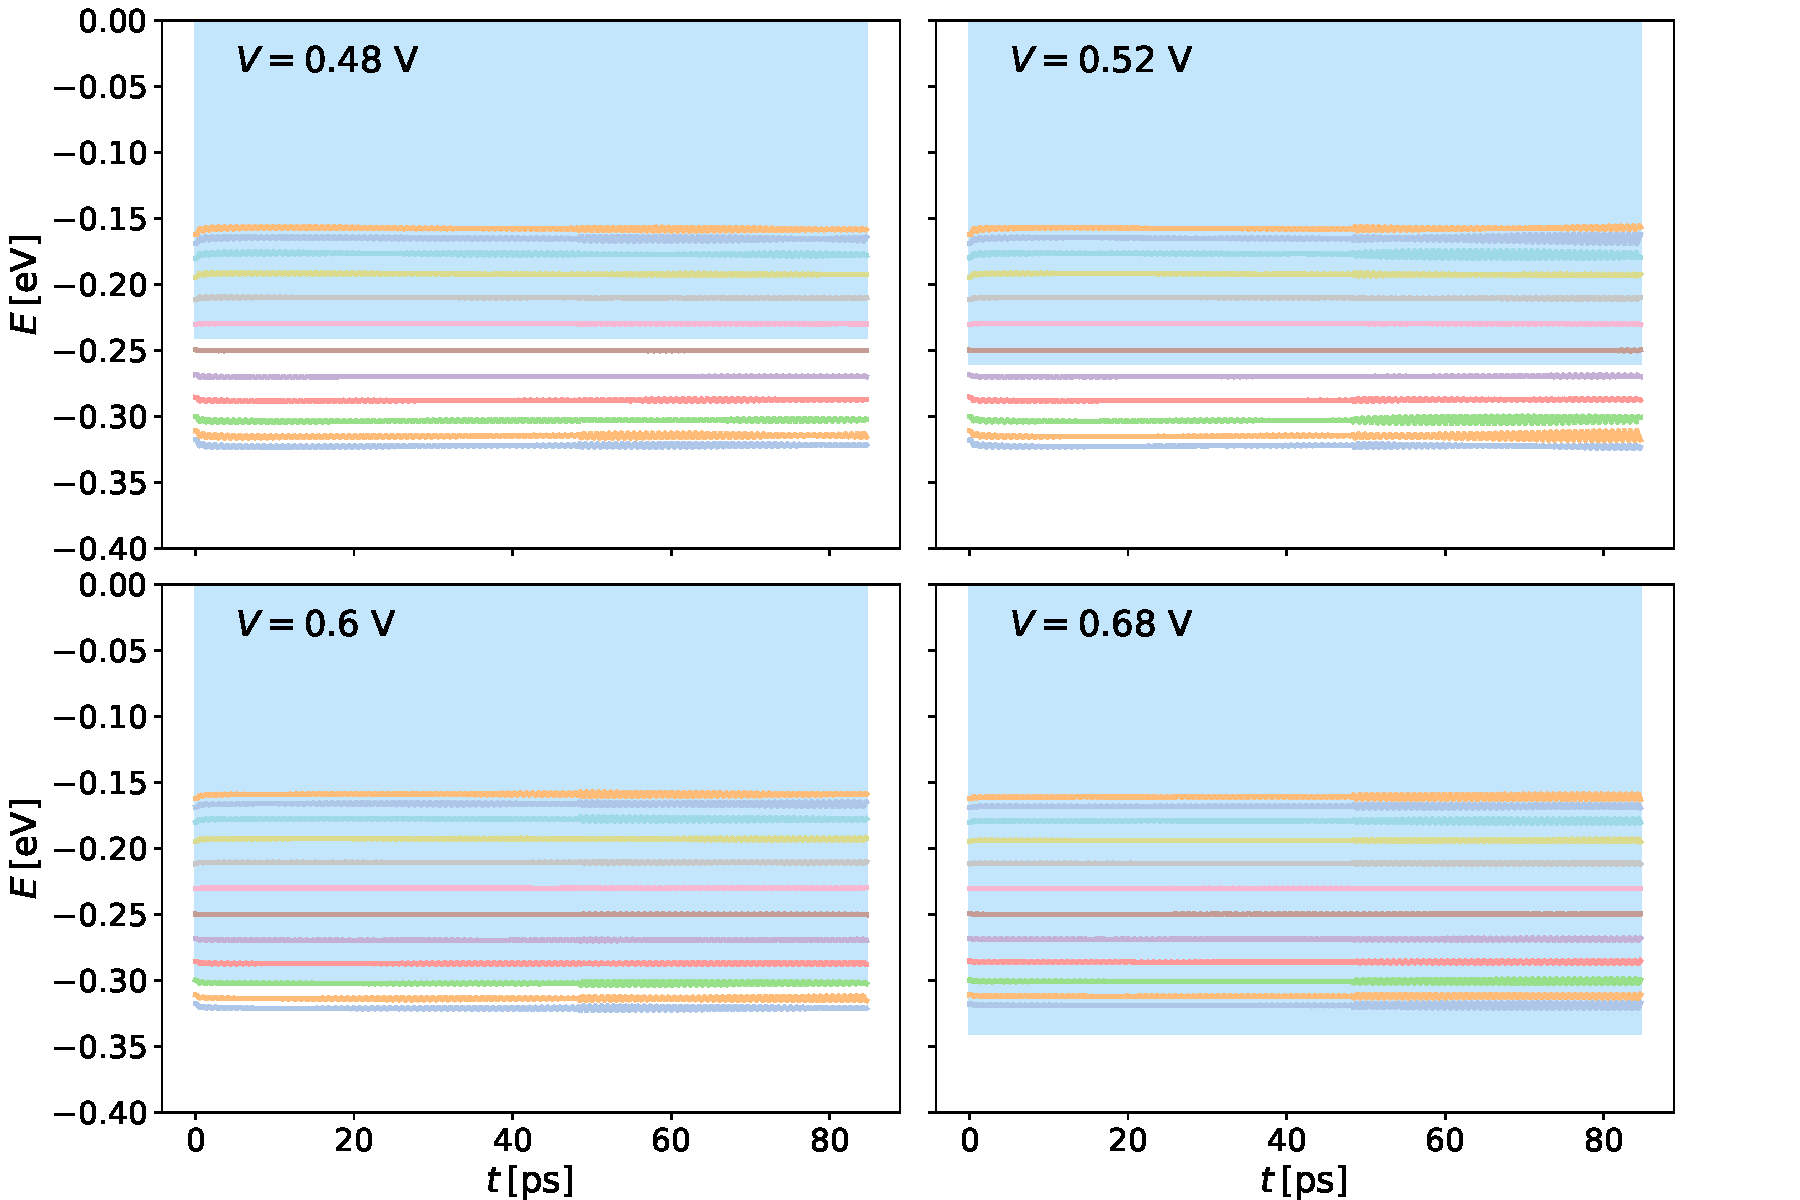
\includegraphics[width=0.9\textwidth]{figs/3x4_0.1/L3x4_spectrumTD_PhAvg_tsoPh0.1.pdf}
\end{figure}
\begin{figure}[!h]
	\centering
	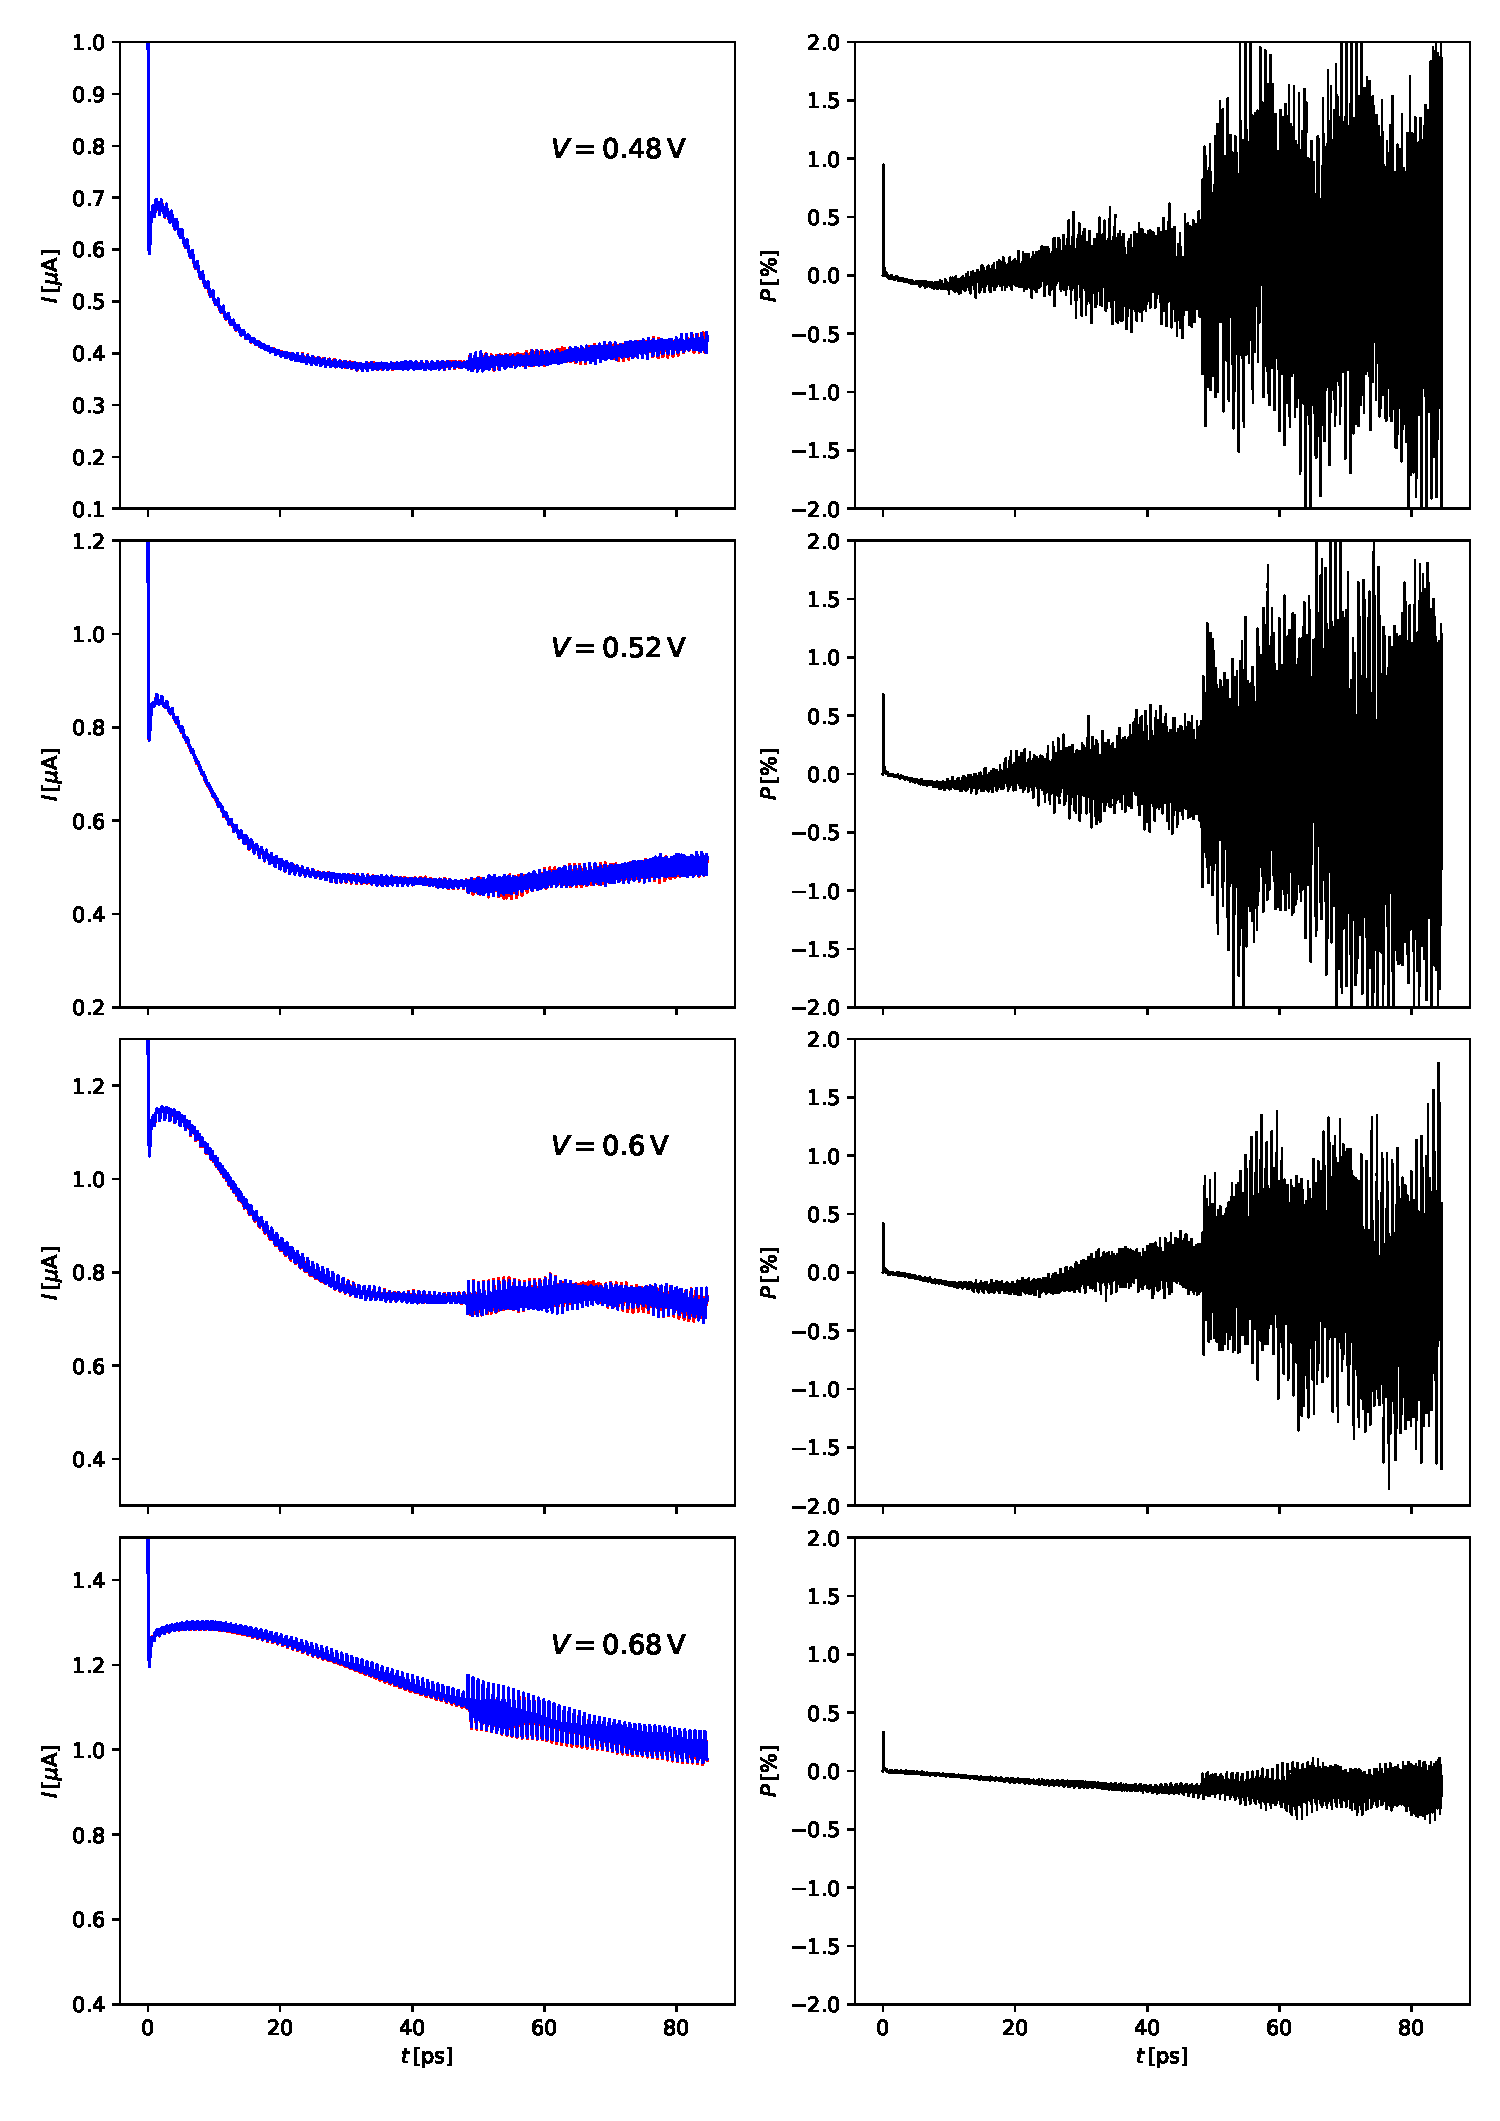
\includegraphics[width=0.9\textwidth]{figs/3x4_0.1/L3x4_currents_MR_allV_tsoPh0.1.pdf}
\end{figure}
\begin{figure}[!h]
	\centering
	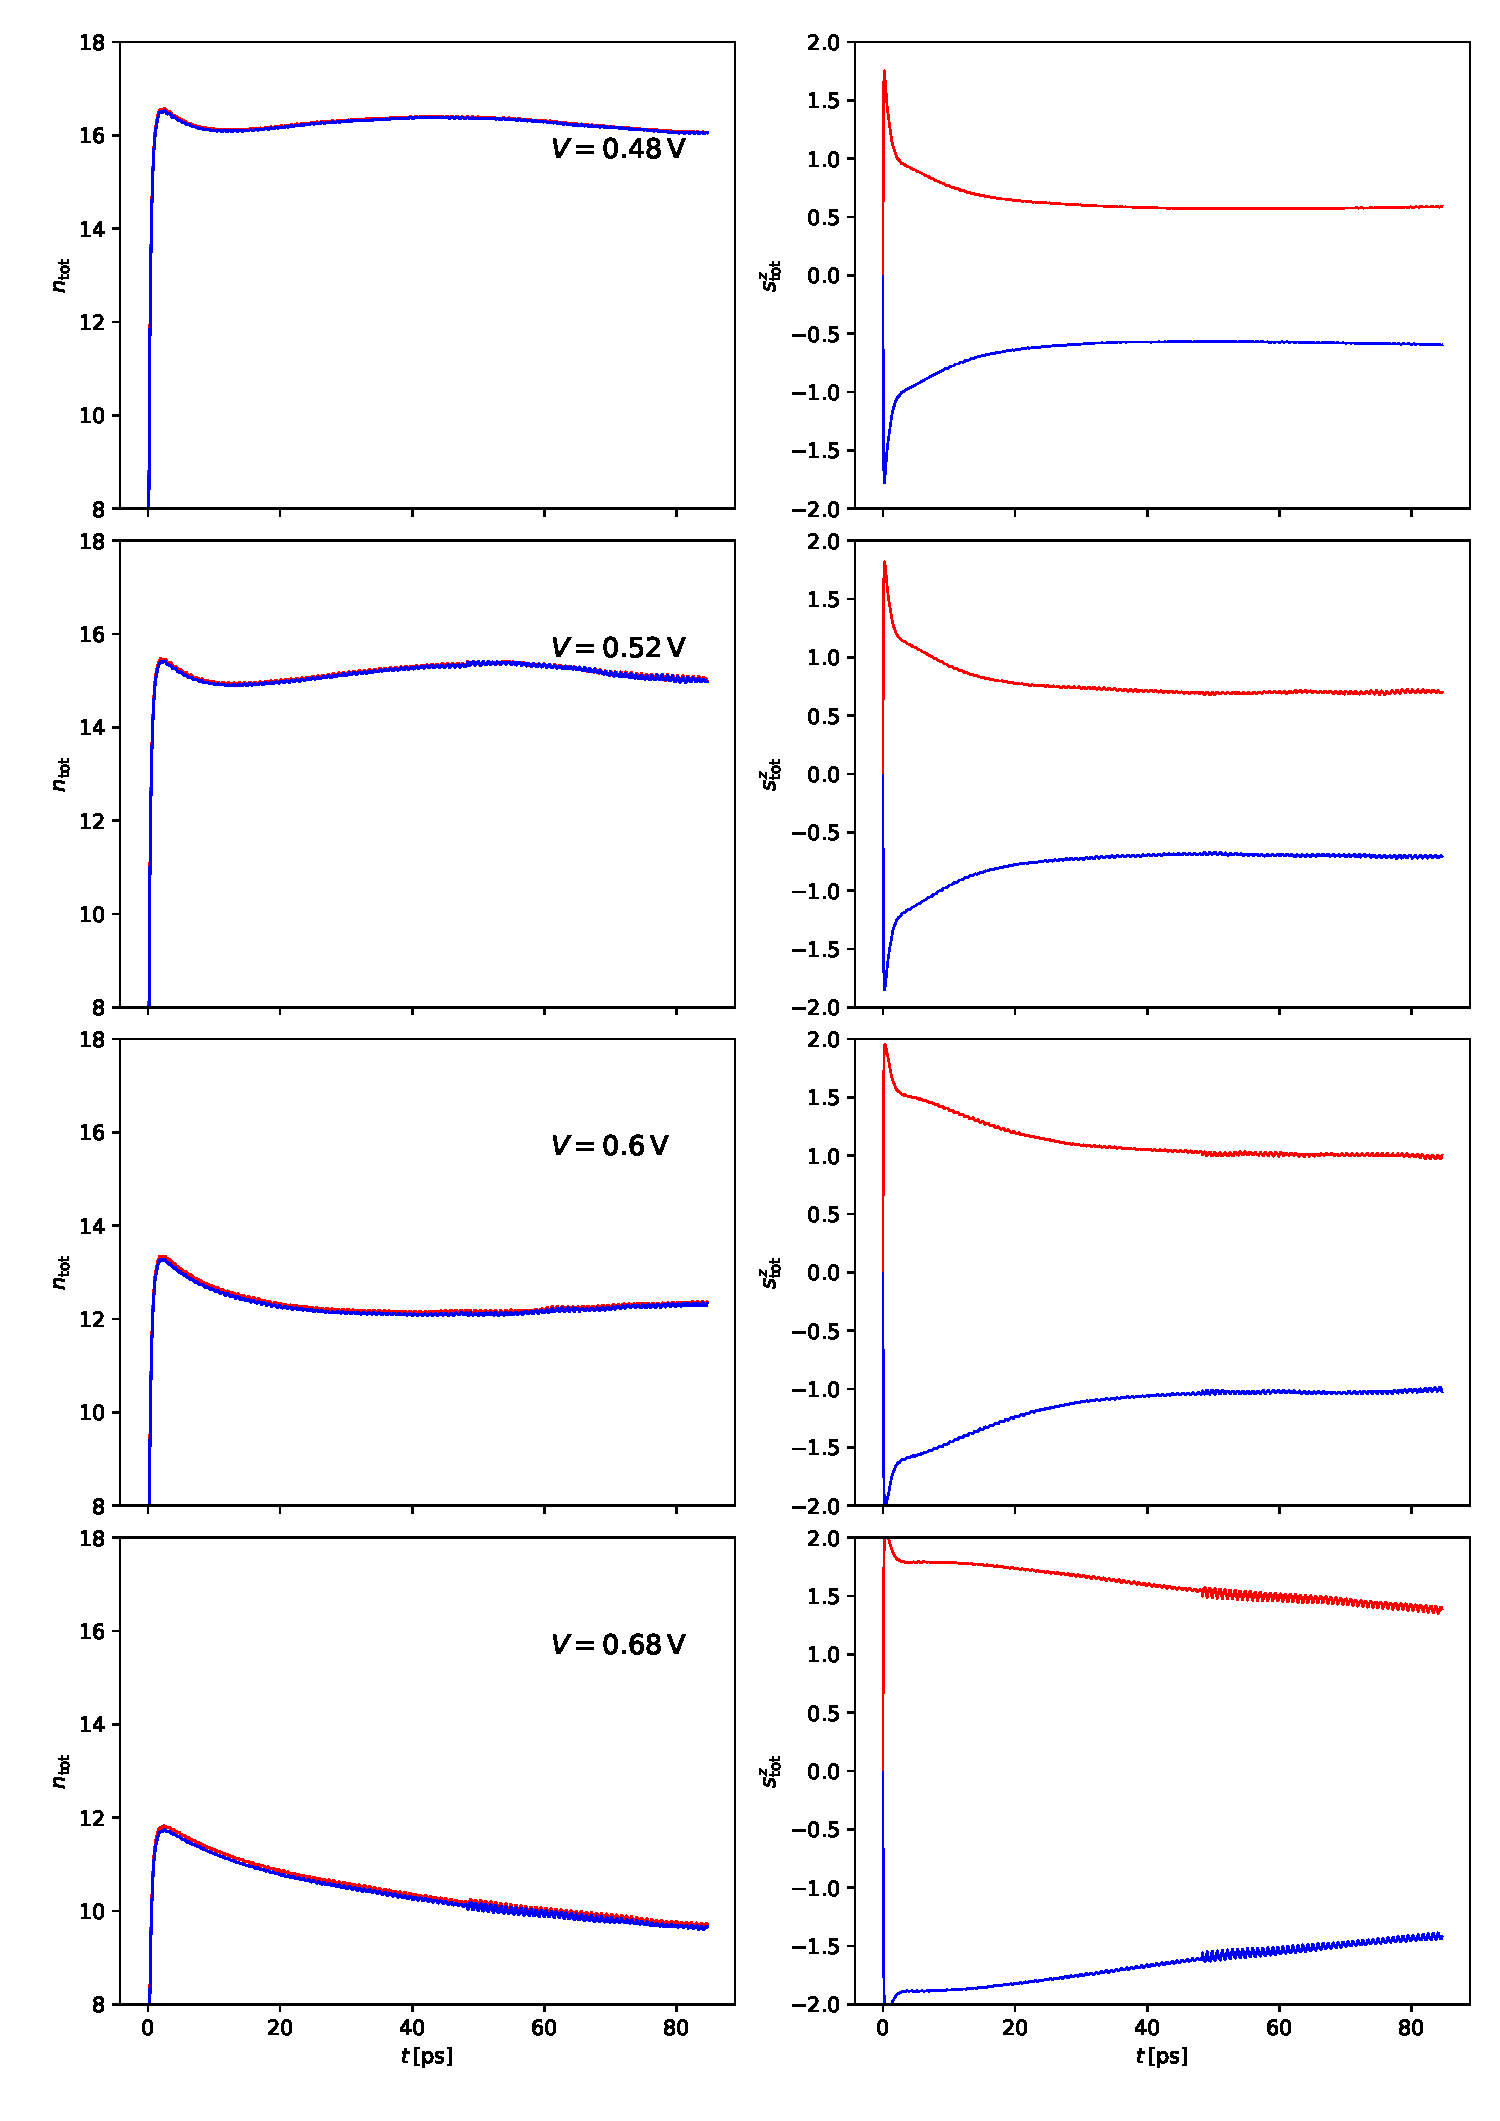
\includegraphics[width=0.9\textwidth]{figs/3x4_0.1/L3x4_charge_sz_tot_allV_tsoPh0.1.pdf}
\end{figure}
\begin{figure}[!h]
	\centering
	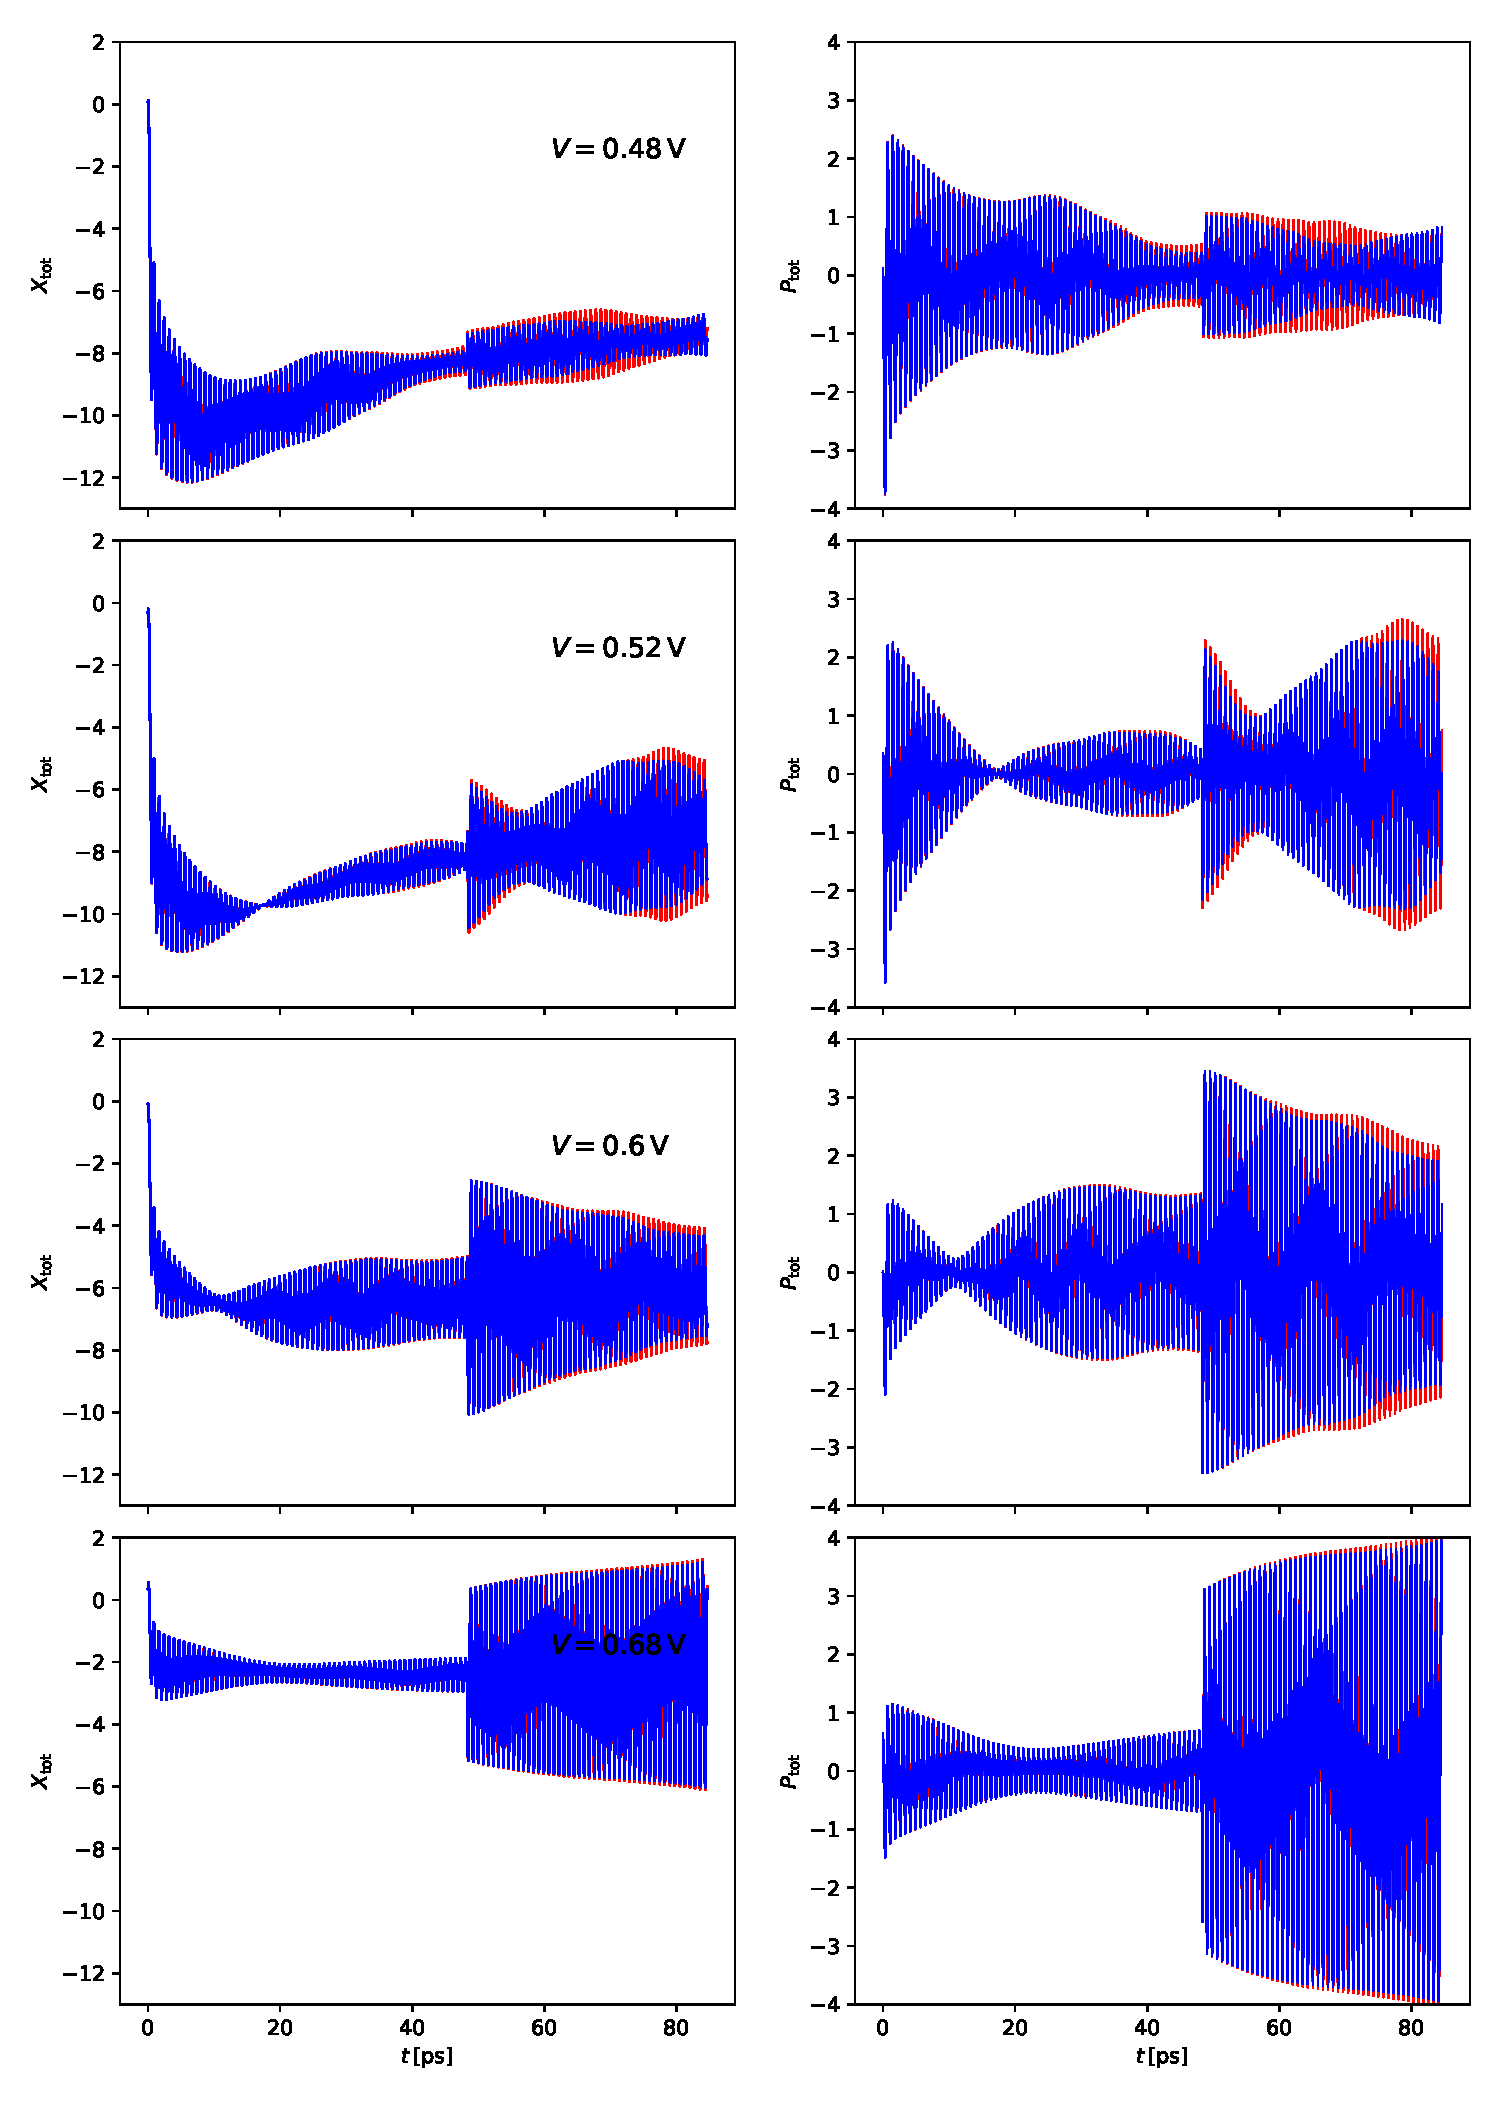
\includegraphics[width=0.9\textwidth]{figs/3x4_0.1/L3x4_phonons_comb_allV_tsoPh0.1.pdf}
\end{figure}
\clearpage
\subsection{Problems}
\begin{itemize}
		\item $\varepsilon_0 = 0$ vs $\varepsilon_0 \neq 0$: 
	\begin{itemize}
		\item   When $\varepsilon=0$, intersite coherences are favored due to the Peierls coupling to the vibrations. These "electronic hopping". Therefore molecule contracts, but because transport is hopping-dominated, the molecular contraction stays. Also there many states that contribute to transport.  
		\item When $\varepsilon <0$, molecule is away from half filling, and therefore there is some kind of hinderence of hopping (pauli principle). Then molecule contracts and expands again. Also, the molecule-lead coupling is a function which decreases with increasing energy. For the smaller voltages investigated here, that also means that electronic transitions from the leads to the molecule are up to an order of magnitude slower than in the case for $\varepsilon=0$.
		Maybe this is one of the reasons for slow relaxation? 
		\item In a previous report from March 1st, the mean force has been computed analytically for a two-site spinless Peierls model. Therein, the force is proportional to the difference in instantaneous occupation of the eigenlevels $F(t)\sim \vert c_+(t)\vert^2-\vert c_-(t)\vert^2$. Generalizing this picture to the problem with more than 2 levels possible?
		\item Importance of $\varepsilon_0$ is a little bit underestimated in Fransson's papers. 
	\end{itemize}
	\item The helix parameters $a$ (helix radius) and $c$ (helix pitch) affect the spin-orbit coupling significantly. In the above computations, these parameters are both set to unity (their values are not reported in any of Franssons papers). Tests have shown that by tuning $a$ and $c$, the values of spin-orbit coupling in hamiltonian can vary over one order of magnitude.
	\item The molecule undergoes a dramatic conformational change when driven out of equilibrium. Among others, the molecular dynamics is qualitatively different for $\varepsilon_0=0$ and $\varepsilon_0\neq 0$. 
%	\item  Implement peierls order parameter
%	\item  Plot PES as a function of collective coords
%	\item  Exp: self assembled monolayers, morphology? Molecular vibrations? Relation to Single molecule models? How to take into account that the dna can fold? How is the length of the system determined so precisely in exp?
	\item Current model does not take into account: Dissociation for $X\rightarrow \infty$, and infinite for $X\rightarrow -\Delta X$ (the equilibrium distance between two monomers). 
	\item  For further analysis: Compute memory kernel from ehrenfest data?
\end{itemize}

\section{Fransson model: Ehrenfest-HEOM analysis}

%\printbibliography
\end{document}


